\ifx\wholebook\relax \else

\documentclass[b5paper]{article}
\usepackage[nomarginpar
  %, margin=.5in
]{geometry}

\addtolength{\oddsidemargin}{-0.05in}
\addtolength{\evensidemargin}{-0.05in}
\addtolength{\textwidth}{0.1in}

\usepackage[en]{../prelude}

\setcounter{page}{1}

\begin{document}

\title{Irrational}

\author{Xinyu LIU
\thanks{{\bfseries Xinyu LIU} \newline
  Email: liuxinyu99@hotmail.com \newline}
  }

\maketitle
\fi

\markboth{Irrational}{A tour of numbers}

\ifx\wholebook\relax
\chapter{Irrational}
\fi

\epigraph{The book of nature is written in the language of mathematics.}{Galileo Galilei}

At noon at the summer solstice (the day is the year's longest) June 21 in 240 BCE, Eratosthenes (276 - 194 BCE), the director of the great library in Alexandria, was talking to a merchant from Syene (now known as Aswān in southern Egypt, lying exactly on the Tropic of Cancer). \enquote{My hometown is hot and dry,} said the merchant, \enquote{We dig very deep wells to draw water; during this season every year, sunlight can reach down to the very bottom of the wells.} Upon hearing this, Eratosthenes noticed the shadow of a monument on the square. Why isn't the sunlight vertical here in Alexandria? Unless the Earth isn't flat, but round, like a sphere. He asked the merchant, \enquote{How long is from Syene to Alexandria?} \enquote{It's about 5,000 stadias} (a stadia is about 158m in Egypt). Eratosthenes measured the lengths of a stick and its shadow, finding the former was 8 times of the latter. He made a calculation based on \cref{fig:eratosthenes-earth}.

\begin{figure}[htbp]
 \centering
 \subcaptionbox{Sunlight falls vertically at summer solstice at Syene on the Tropic Cancer. \label{fig:eratosthenes-earth}}{\includegraphics[scale=0.35]{img/eratosthenes-earth}}
 \subcaptionbox{Sunlight falls at an angle of $\alpha$ from the vertical at Alexandria. \label{fig:atan8}}{\includegraphics[scale=0.32]{img/atan8}}
 \caption{Eratosthenes made the measurement of the size of Earth.}
\end{figure}

\index{Eratosthenes}
Sunlight falls vertically at noon at summer solstice on the Tropic Cancer, hence reaches down to the very bottom of the wells in Syene. Eratosthenes could find the angle of the sunlight to the vertical at Alexandria through \cref{fig:atan8}.
%% 这相当于今天高中数学中的反正切$\arctan(\frac{1}{8})$。
As the Babylonian degree hadn't been adopted by the Greeks by that time, according to Eratosthenes, the angle was a fiftieth of a circle, which was about $7.2\degree$. He correctly assumed the Sun’s distance to be very great; its rays therefore are practically parallel when they reach Earth. If the Earth is round, then the angle between Syene and Alexandria to the center of Earth equals the angle of sunlight and earth as they are corresponding angles (the two angles labeled $\alpha$ in \cref{fig:eratosthenes-earth}). As this angle is a fiftieth of a circle, the distance between Syene and Alexandria is a fiftieth of the circumstance of the Earth. Eratosthenes hence calculated the circumstance to be $50 \times 5,000 = 250,000$ stadias, which was approximately $250 \times 158 = 39,500 \approx 40,000$ kilometers. This is quite close to the circumstance of the equator of Earth, which is 40,075 kilometers measured by satellite today. None of Eratosthenes's books survived today\footnote{The only supposed surviving book \emph{Catasterisms} is about constellation, but has been doubted by some scholars.}; his mathematical work is known principally from the writings of the Greek geometer Pappus of Alexandria. Eratosthenes became director of the great library of Alexandria from 235 BCE, his measurement to the Earth happened likely during this period\cite{Walkup2005}. The distance between Syene and Alexandria was critical to the result; 5,000 stadias was mostly a rough number. Eratosthenes might verify this number in multiple ways, including confirming from the merchant and measuring the map. Both Syene and Alexandria were on the bank of Nile river; the Nile flooded regularly every year, changing the landscape around it. The Egypt re-surveyed the lands along the Nile and updated the map after the flood every year. Besides, there are different opinions about the exact length of a Stadia. Nevertheless, Eratosthenes's reasoning and measurement of the Earth over 2,000 years ago is definitely astonishing.

\begin{figure}[htbp]
 \centering
 \includegraphics[scale=0.35]{img/eratosthenes}
 % https://commons.wikimedia.org/wiki/File:Eratosthenes_Teaching_in_Alexandria_(Bernardo_Strozzi,_Montreal).jpg
 \caption{Eratosthenes teaching in Alexandria, by Bernardo Strozzi, 1635.}
 \label{fig:eratosthenes}
\end{figure}

Alexandria was the capital of Egypt from its founding by Alexander the Great in 332 BCE. It's the center of Hellenic scholarship and science. Eratosthenes's measurement to the size of Earth set a remarkable example of Greek geometry; it's a successful application demonstrating the strength of geometry. The Greeks had tradition of rigorous reasoning on top of which they developed geometry. Despite the lack of positional numeral system, they discovered irrationals after giving numbers geometric interpretation.

\section{All is number}
\index{Pythagoras}
Pythagoras was inspired by his discovery that music was ruled by ratio of numbers, although they were commonly thought unrelated. He asserted, \emph{\enquote{all is number}}, and was the first who studied the nature with numbers. Pythagoras was born in the island of Samos, off the coast of modern Turkey. Pythagoras might have leaned from Thales of Miletus. With Thales suggestion, he went to Egypt to learn more about mathematics in about 535 BCE. He spent 10 years in Egypt till the Persian empire conquered Egypt in 525 BCE. He was taken prisoner to Babylon with the army. Pythagoras learned mathematics and astronomy from the Babylonians. He might also arrive in India\cite{HanXueTao16}.

Pythagoras returned his hometown Samos after long journey abroad in around 520 BCE. He founded a school and began to give lectures. Two years later, he left Samos, possibly because he disagreed with the local tyranny. He arrived in the Greek colony of Croton (southern Italy in present day), where he earned trust and admiration from people. He founded the philosophical and religious school that had many followers. Several prominent members of his school were women. The school was devoted to study astronomy, geometry, number, and music, known as \emph{quadrivium}, which influenced the education in the west over 2000 years\cite{StepanovRose15}. The Pythagoreans believed the celestial bodies, planetary motions, geometric objects, and musics all based on numbers. The Pythagorean society at Croton was attacked due to political conflict in around 497 BCE. Some said Pythagoras was killed while others said he escaped to Metapontum and died there\cite{MKlein1972}.

\index{figurate number}
The Pythagoreans studied the numbers and the their relations to nature. They developed the early number theory, one of the most important branches in mathematics. The Pythagreans classified natural numbers, defining even and odd numbers, prime and composite numbers, and so on. They discovered many \emph{figurate} numbers when formed geometric figure with small pebbles\footnote{The word calculus in Latin means `pebble'.\cite{HanXueTao16}}.

\begin{figure}[htbp]
\centering
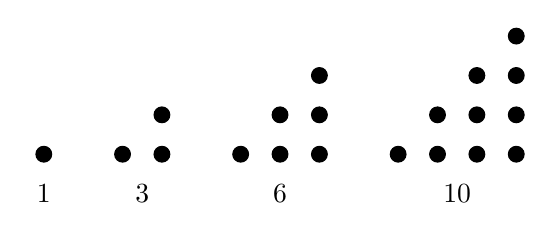
\begin{tikzpicture}[scale=0.5]
\filldraw (0, 0) circle (0.2);
\draw (0, -1) node{1};
\filldraw (2, 0) circle (0.2)
          (3, 0) circle (0.2)   (3, 1) circle (0.2);
\draw (2.5, -1) node{3};
\filldraw (5, 0) circle (0.2)
          (6, 0) circle (0.2)   (6, 1) circle (0.2)
          (7, 0) circle (0.2)   (7, 1) circle (0.2)   (7, 2) circle (0.2);
\draw (6, -1) node{6};
\filldraw (9, 0) circle (0.2)
          (10, 0) circle (0.2)    (10, 1) circle (0.2)
          (11, 0) circle (0.2)    (11, 1) circle (0.2)    (11, 2) circle (0.2)
          (12, 0) circle (0.2)    (12, 1) circle (0.2)    (12, 2) circle (0.2)    (12, 3) circle (0.2);
\draw (10.5, -1) node{10};
\end{tikzpicture}
\caption{Triangular number}
\label{fig:triangular-num}
\end{figure}

\begin{figure}[htbp]
\centering
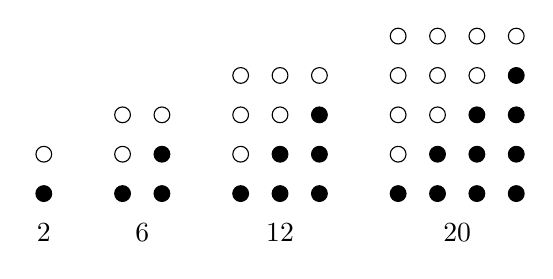
\begin{tikzpicture}[scale=0.5]
\draw (0, 1) circle (0.2);
\filldraw (0, 0) circle (0.2);
\draw (0, -1) node{2};

\draw (2, 1) circle (0.2)   (2, 2) circle (0.2)
      (3, 2) circle (0.2);
\filldraw (2, 0) circle (0.2)
          (3, 0) circle (0.2)   (3, 1) circle (0.2);
\draw (2.5, -1) node{6};

\draw (5, 1) circle (0.2)   (5, 2) circle (0.2)   (5, 3) circle (0.2)
      (6, 2) circle (0.2)   (6, 3) circle (0.2)
      (7, 3) circle (0.2);
\filldraw (5, 0) circle (0.2)
          (6, 0) circle (0.2)   (6, 1) circle (0.2)
          (7, 0) circle (0.2)   (7, 1) circle (0.2)   (7, 2) circle (0.2);
\draw (6, -1) node{12};

\draw (9, 1) circle (0.2)   (9, 2) circle (0.2)   (9, 3) circle (0.2)   (9, 4) circle (0.2)
      (10, 2) circle (0.2)   (10, 3) circle (0.2)   (10, 4) circle (0.2)
      (11, 3) circle (0.2)   (11, 4) circle (0.2)
      (12, 4) circle (0.2);
\filldraw (9, 0) circle (0.2)
          (10, 0) circle (0.2)    (10, 1) circle (0.2)
          (11, 0) circle (0.2)    (11, 1) circle (0.2)    (11, 2) circle (0.2)
          (12, 0) circle (0.2)    (12, 1) circle (0.2)    (12, 2) circle (0.2)    (12, 3) circle (0.2);
\draw (10.5, -1) node{20};
\end{tikzpicture}
\caption{Oblong (rectangle) number)}
\label{fig:oblong-num}
\end{figure}

\Cref{fig:triangular-num} and \cref{fig:oblong-num} show the triangular numbers and oblong numbers. It's easy to see a oblong number is two times of a triangular number, and a triangular number is the sum of the first $n$ natural numbers. In this way, the Pythagoreans discovered the formula to the sum of progressive number series:

\[
1 + 2 + 3 + ... + n = \frac{1}{2}n(n+1)
\]

By arranging odd numbers into the shape of gnomon\footnote{The term `gnomon' originally comes from the Babylonians, meaning the stick whose shadow was used to tell time. It changed to mean a carpenter's square in Pythagoras's time: one cut off a small square at a corner of a big square. Later Euclid extended it from square to parallelogram(\cite{MKlein1972}, p31).} as shown in \cref{fig:gnomon-num}, the Pythagoreans found the first $n$ gnomon shapes form a square, as in \cref{fig:square-num}, whence they discovered the formula to the sum of $n$-odd numbers.

\[
1 + 3 + 5 + ... + (2n - 1) = n^2
\]

\begin{figure}[htbp]
\centering
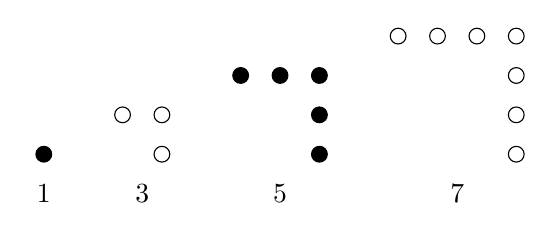
\begin{tikzpicture}[scale=0.5]
\filldraw (0, 0) circle (0.2);
\draw (0, -1) node{1};

\draw (2, 1) circle (0.2)
      (3, 0) circle (0.2)   (3, 1) circle (0.2);
\draw (2.5, -1) node{3};

\filldraw (5, 2) circle (0.2)   (6, 2) circle (0.2)   (7, 2) circle (0.2)
          (7, 0) circle (0.2)   (7, 1) circle (0.2);
\draw (6, -1) node{5};

\draw (9, 3) circle (0.2)   (10, 3) circle (0.2)   (11, 3) circle (0.2)   (12, 3) circle (0.2)
      (12, 0) circle (0.2)    (12, 1) circle (0.2)    (12, 2) circle (0.2);
\draw (10.5, -1) node{7};
\end{tikzpicture}
\caption{Gnomon number}
\label{fig:gnomon-num}
\end{figure}

\begin{figure}[htbp]
\centering
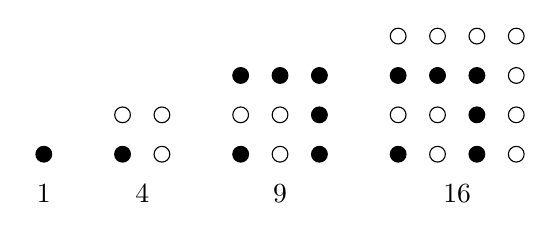
\begin{tikzpicture}[scale=0.5]
\filldraw (0, 0) circle (0.2);
\draw (0, -1) node{1};

\filldraw (2, 0) circle (0.2);
\draw (2, 1) circle (0.2)
      (3, 0) circle (0.2)   (3, 1) circle (0.2);
\draw (2.5, -1) node{4};

\filldraw (5, 0) circle (0.2);
\draw (5, 1) circle (0.2)
      (6, 0) circle (0.2)   (6, 1) circle (0.2);
\filldraw (5, 2) circle (0.2)   (6, 2) circle (0.2)   (7, 2) circle (0.2)
          (7, 0) circle (0.2)   (7, 1) circle (0.2);
\draw (6, -1) node{9};

\filldraw (9, 0) circle (0.2);
\draw (9, 1) circle (0.2)
      (10, 0) circle (0.2)   (10, 1) circle (0.2);
\filldraw (9, 2) circle (0.2)   (10, 2) circle (0.2)   (11, 2) circle (0.2)
          (11, 0) circle (0.2)   (11, 1) circle (0.2);
\draw (9, 3) circle (0.2)   (10, 3) circle (0.2)   (11, 3) circle (0.2)   (12, 3) circle (0.2)
      (12, 0) circle (0.2)    (12, 1) circle (0.2)    (12, 2) circle (0.2);
\draw (10.5, -1) node{16};
\end{tikzpicture}
\caption{Decompose a square number into gnomon numbers.}
\label{fig:square-num}
\end{figure}

The Pythagoreans thus interpreted geometric shapes as numbers. In fact, they were enthusiastic to explain almost everything with numbers and believed \emph{all is number}. This began their attempt to lay the foundation of geometry on numbers.

\section{Pythagorean theorem}

\begin{figure}[htbp]
 \centering
 \includegraphics[scale=0.35]{img/harvest-scene}
 \caption{Rope meter in \emph{Harvest Scenes}, Tomb of Menna, by Charles K. Wilkinson. Menna was a high-ranking official during the reign of Pharaoh Thutmose IV of 18th Dynasty (about 1400 - 1352 BCE). }
 %% https://www.metmuseum.org/art/collection/search/548574
 \label{fig:rope-meter}
\end{figure}

\index{Pythagorean theorem}
Pythagorean theorem, the well-known geometric theorem, was commonly attributed to Pythagoras. A legend said Pythagoras was so satisfied and proud with the discovery of the theorem, that he sacrificed a hecatomb (100 head of cattle). However, it was mostly not true because Pythagoras was a vegetarian. The Pythagorean school, in modern terms, is a monastery, where all members took strict vows of secrecy, and all new mathematical results for several centuries were attributed to his name. Thus, not only is the first proof of the theorem not known, there is also some doubt that Pythagoras himself actually proved the theorem that bears his name. The Pythagorean theorem was probably independently discovered in several different cultures. For example, the Babylonian tablet as shown in \cref{fig:babylonian-yale} in chapter 3 was around 1900 - 1600 BCE. There were also tablets inscribed with table of Pythagorean triples. The Egyptians made measurement with ropes (known as rope meter as shown in \cref{fig:rope-meter}). It was said they tied knots in a rope, divided it into segments of 3, 4, and 5, and used these segments to form a right-angled triangle. However, there were not any documents or evident of this saying\citepage[16页]{MKlein-1972}. The theorem is mentioned in the Baudhayana \emph{Sulba-sutra} of India, which was written between 800 and 400 BCE. In the \emph{Nine Chapters}, compiled in the 1st century CE in China, the title of the last chapter is `勾股', meaning the two legs of a right triangle\footnote{This term comes from an earlier book \emph{Zhou Bi Suan Jing} (The Arithmetical Classic of the Gnomon and the Circular Paths of Heaven), compiled in the 1st century BCE, which contains a dialogue between the Duke of Zhou and Shang Gao dating back to the Western Zhou Dynasty (c. 11th century BCE). This dialogue mentioned, ``勾: 3, 股: 4, 弦(hypotenuse): 5''.}. It was dedicated to this theorem with 24 problems and their solution. When later mathematicians, such as Zhao Shuang and Liu Hui, commenting it around the 3rd century, they offered proofs\footnote{Some argue whether these are proofs or demonstration.} by cutting up the squares on the legs of the right triangle and rearranging them (``tangram style'') to correspond to the square on the hypotenuse.

\begin{figure}[htbp]
 \centering
 \subcaptionbox{Logo of the Chinese Mathematical Society (CMS) \label{fig:cms-logo}}{\includegraphics[scale=0.5]{img/cms}} \quad
 \subcaptionbox{Zhao Shuang's Chord diagram \label{fig:zhaoshuang}}{\includegraphics[scale=0.2]{img/zhaoshuang}}
 \caption{The logo of Chinese Mathematical Society comes from Zhao Shuang's Chord diagram; it which was also used as the logo of International Congress of Mathematicians (ICM) 2002. \label{fig:cms-zhaoshuang}}
\end{figure}

Since discovered, the theorem has fascinated people for nearly 4,000 years. More than 300 proofs has been developed, including Zhao Shuang's diagram (\cref{fig:cms-zhaoshuang}), the proof shown in \cref{fig:pythagoras-pww} is said attributed to Pythagoras, the famous \enquote{windmill} proof by Euclid, the ones by the Italian artist-inventor Leonardo da Vinci (1452 - 1519, \cref{fig:pythagoras-pww}), and even U.S. president James Garfield (1831 - 1881, \cref{fig:garfield}).

\begin{figure}[htbp]
 \centering
 \includegraphics[scale=0.25]{img/pythagoras-pww}
 \caption{The proof that is said by Pythagoras. \label{fig:pythagoras-pww}}
\end{figure}

\index{Pythagorean theorem!Leonardo da Vinci's proof}
Leonardo da Vinci's duplicated the original right triangle to two copies: one was reflective against the line through the point at the right angle; the other moves to the bottom of the big square as shown in \cref{fig:davinci}. If `flip' the quadrilateral above the `T' shape, one gets two identical hexagons of the same area. Each substitute two copies of the original right triangle gives the same remaining area, which is $a^2 + b^2 = c^2$. \Cref{qn:pythagoras-thm-garfield} asks to explain president Garfield's proof.

\begin{figure}[htbp]
 \centering
 \includegraphics[scale=0.3]{img/davinci}
 \caption{Leonardo da Vinci's proof to the Pythagorean theorem \label{fig:davinci}}
\end{figure}

The remarkable Pythagorean theorem is the source of three great streams of mathematical thoughts\cite{Stillwell-2010}: (1) numbers, by searching the whole numbers satisfying Pythagoras theorem (known as Pythagorean triples), the Greeks started the study of number theory; (2) geometry, it an important geometric theorem about right triangle and squares; (3) infinity, by applying the theorem to Euclidean algorithm, the Greeks discovered a totally new family of numbers, the irrationals.

\section{Number theory}
\index{Pythagorean triples}
The sum of two squares is not necessarily a square, for example, $3^2 + 5^2 = 34$ is not a square number. The Greeks define whole numbers $(a, b, c)$ as a Pythagorean triple. Different cultures independently discovered triples like $3^2 + 4^2 = 5^2$ and $5^2 + 12^2 = 13^2$; some Babylonian tablets list long table of Pythagorean triples. But how to find such triples systematically? Are there finite or infinite Pythagorean triples? Both problems were completely solved by Euclid. First, Euclid simplified the problem that if $a^2 + b^2 = c^2$, then any multiples of $a, b, c$ are Pythagorean triples too, because:

\begin{align*}
(ka)^2 + (kb)^2 &= k^2(a^2 + b^2) & \text{distributive law} \\
  &= k^2c^2 & \text{by } a^2 + b^2 = c^2 \\
  &= (kc)^2
\end{align*}

Conversely, if $a, b$ have some common factor $k \ne 1$, then $k$ is also a factor of $c$. In the same way, since $a^2 = c^2 - b^2$, the common factor $k$ of $b, c$ is also a factor of $a$. It turns out we only need to search those Pythagorean triples consists of coprime $a, b, c$ (the only common factor of them is 1, i.e., $(a, b) = (b, c) = 1$, see \ref{sec:gcd-minus}), and their multiplies are all Pythagorean triples. For example, each of (12, 16, 20) is even, they have common factor of 2; halving them gives `simpler' triple of (6, 8, 10); halving again gives (3, 4, 5); they are coprime and can't be simplified any more. We may call such a triple the `simplified Pythagorean triple'. Because the parity of $a$ and $a^2$ are same: the square of odd is odd; the square of even is even. If $a, b$ has different parity (an even and an odd), then $c$ must be odd. Euclid further ruled out the case the both $a, b$ are odd, because:

\begin{align*}
a^2 + b^2 &= (2m + 1)^2 + (2n + 1)^2 & \text{both }a, b\text{ are odd} \\
  &= 4m^2 + 4m + 1 + 4n^2 + 4n + 1 & \text{expand} \\
  &= 4(m^2 + m + n^2 + n) + 2 = 4k + 2 & \text{let } k = m^2 + m + n^2 + n
\end{align*}

The remainder of this value divided by 4 is 2, but no matter $c$ is even or odd, the remainder of $c^2$ divided by 4 can not be 2, for even, $(2k)^2 = 4k^2$ can be divided by 4; for odd, $(2k + 1)^2 = 4(k^2 + k) + 1$ gives remainder 1. Therefore, $a$ and $b$ can not both be odd, but an odd and an even. We may let one, for example the first, be the even and the other be odd. Now the problem turns to find those Pythagorean triples, consisting numbers being coprime and the first being even. The solution was given as Lemma 1 in Book X of \emph{The Elements}\footnote{We use algebraic symbols here for easy understanding; Euclid stated in geometric language\citepage[p330]{Elements}.}

\begin{lemma}[Euclid, Lemma 1, Book X, The Elements] \label{thm:pythagoras-triples}
For equation $x^2 + y^2 = z^2$, where $x, y, z$ are coprime and $x$ is even, \underdot{all} solutions in natural numbers are:
\be
\begin{cases}
x = 2mn \\
y = m^2 - n^2 \\
z = m^2 + n^2
\end{cases}
\ee
where $m > n$ are natural numbers in opposite parity.
\end{lemma}

This lemma covers \emph{all} solutions; there are not any Pythagorean triples out of scope. In other words, it is \emph{necessary and sufficient}.

\begin{proof}
We first show any such $x, y, z$ is a Pythagorean triple:

\begin{align*}
x^2 + y^2 &= (2mn)^2 + (m^2 - n^2)^2 \\
  &= 4m^2n^2 + m^4 + n^4 - 2m^2n^2 & \text{expand} \\
  &= m^4 + n^4 + 2m^2n^2 = (m^2 + n^2)^2 &\text{perfect square formula} \\
  &= z^2
\end{align*}

Conversely, we show any Pythagorean triple is in this form. Move $y^2$ in the left side of $x^2 + y^2 = z^2$ to the right:
\begin{align}
x^2 &= z^2 - y^2 = (z + y)(z - y) &\text{difference of squares} \label{eq:x-as-z-pm-y} \\
(\frac{x}{2})^2 &= (\frac{z + y}{2}) (\frac{z - y}{2}) &\text{both sides divided by 4}
\end{align}

$x$ is even, $y, z$ are odd, hence $z \pm y$ are odd. It follows that both $\dfrac{x}{2}$ on the left and $\dfrac{z \pm y}{2}$ on the right are whole numbers. Moreover, since $z, y$ are coprime, $\dfrac{z + y}{2}$ and $\dfrac{z - y}{2}$ are coprime (by \cref{qn:coprime-of-half-a-pm-b}). For two coprime numbers, if their product is a square, then each is a square (by \cref{qn:coprime-product-as-square}), thereby,

\begin{align*}
\frac{z+y}{2} &= m^2 \\
\frac{z-y}{2} &= n^2
\end{align*}

where $m > n$ are natural numbers. Adding the two equations cancels $y$ and gives $z = m^2 + n^2$; subtracting the two equations cancels $z$ and gives $y = m^2 - n^2$; finally substituting into \cref{eq:x-as-z-pm-y} gives: $x^2 = 2m^2 2n^2$, hence $x = 2mn$.
\end{proof}

For example, taking $m = 2, n = 1$ gives the triple of (3, 4, 5); taking $m = 3, n = 2$ gives the triple of (12, 5, 13). All Pythagorean triples are:

\be
x = 2mnr, \quad y = r(m^2 - n^2), \quad z = r(m^2 + n^2)
\ee

where $r$ any natural number.

\begin{figure}[htbp]
 \centering
 \includegraphics[scale=0.6]{img/Euclid}
 \caption{Euclid, c. 325 - 265 BCE}
 \label{fig:Euclid}
\end{figure}

\begin{mdframed}

\index{Euclid} \index{The Elements}
Euclid of Alexandria was the most prominent mathematician of antiquity best known for his treatise on mathematics \emph{The thirteen books of Euclid's elements}, or \emph{The Elements} for short. It influenced the development of Western mathematics for more than 2,000 years. However little is known of Euclid's life except that he taught at Alexandria in Egypt. Proclus, the last major Greek philosopher, who lived around 450 CE wrote a story about Euclid: Ptolemy I of Alexandria (king of Egypt, 323 - 283 BCE) grew frustrated in learning {\em The Elements}; he asked Euclid if there was a shorted way to study geometry, Euclid replied \emph{there was no royal road to geometry.} This becomes the learning maxim of eternal. Another story by Stobaeus said a student, after learning the first theorem, asked \enquote{What shall I get by learning these things?} Euclid said \enquote{Give him three pence since he must make gain out of what he learns.} Euclid disagreed with the narrow practical view of learning\cite{Elements}.

From ancient times to present, {\em The Elements} has been used as a perfect example of correct reasoning. Many results in {\em The Elements} originated from earlier mathematicians, such as Eudoxus and Theaetetus. It was Euclid, who arranged them in order and perfected what had been only loosely proved by his predecessors. More than a thousand editions have been published, making it one of the most popular books after the Bible. {\em The Elements} is still widely taught in school\footnote{The most popular version was edited by the French mathematician Legendre (1752 - 1833).} as one of the basic way to train logic reasoning\cite{HanXueTao16}.
\end{mdframed}

\index{prime}
Euclid's lemma completely solved the equation of $x^2 + y^2 = z^2$ in Pythagorean triples. It's natural to extend the equations to $x^3 + y^3 = z^3$, $x^4 + y^4 = z^4$, or generally, equation of $x^n + y^n = z^n$, where the integer $n \geq 3$. However, people encountered exceptional difficulties with them; it seems, except for the trivial one $xyz = 0$, there was no integral solution. It was not until the 17 century, about 1,800 years later, Fermat achieved some result for $n = 4$ (see \cref{sec:FLT-4}). The problem of Pythagorean triples demonstrated what is typically concerned in number theory: the study of numbers and their properties. For a long time, people called it `arithmetic', for example, Diaphanous's classic work \emph{Arithmetica} and Gauss's famous work \emph{Disquisitiones Arithmeticae}. It deals with the things like parity (even and odd), divisibility, prime numbers, factors, remainders, and so on. In the study of figurate numbers, the Greeks recognized the rectangle numbers, for example $12 = 3 \times 4$ could be formed with three rows and four columns of pebbles. It arose the notion of factor, that the sides corresponded to the factors of the rectangle number; and there were multiple factors, because $12 = 3 \times 4 = 2 \times 6$, 2, 3, 4, and 6 are all factors of 12. Some numbers were not rectangle numbers, like 5, which could only be formed with a row or a column of five pebbles\footnote{Obviously, the Greeks distinguished segment from rectangle since they did not accept $1 \times 5$ or $5 \times 1$ as a rectangle number.}. This led to the notion of prime number: a prime $p$ can be divided only by 1 and itself. Prime numbers are basic bricks to form other composite numbers (through multiplication), the first prime numbers are 2, 3, 4, 7, 11, ... It naturally arose questions: (1) As the bricks to other numbers, how many prime numbers are there? finitely or infinitely? (2) Are there any patterns of prime numbers? is there a formula or an algorithm to generate prime numbers? The first question was, again, answered by Euclid, while the second was much harder; it was Eratosthenes who took the first step to the second question.

The Greeks tried to avoid using the notion of infinity after Zeno's paradoxes. Aristotle thought all Zeno's paradoxes concerning infinity. He distinguished {\em potential} and {\em actual} infinities. Potential infinity is a process that never stops; it can be a collection of \enquote{things} that continues without terminating, going on or repeating itself over and over again with no recognizable ending point. The obvious example is natural numbers of 1, 2, 3, ... given any number $n$, there always exists another number $n + 1$ to proceed. In geometry, a line can be extended any long as needed. Actual infinity involves never-ending sets or \enquote{things} within a space that has a beginning and end; it is a series that is technically \enquote{completed} but consists of infinitely many members. According to Aristotle, actual infinities cannot exist because they are paradoxical. It is impossible to say that you can always \enquote{take another step} or \enquote{add another member} in a completed set with a beginning and end, unlike a potential infinite. It was ultimately Aristotle’s rejection of the actual infinite that allowed him to refute Zeno’s paradox. Aristotle's opinion was widely accepted, that Euclid never used the term of `infinity' or `infinitely many' in \emph{The Elements}. Nevertheless, he successfully showed there are `infinitely many' prime numbers in our modern view; his proof was thought to be one of the most beautiful proofs in history.

\begin{theorem}[Euclid, Proposition 20, Book IX, The Elements]
Prime numbers are more than any assigned multitude of prime numbers.
\end{theorem}

Euclid carefully avoided using term of infinitely many, but stated, \enquote{more than any assigned ...}. This is common treatment in many places in \emph{The Elements}. We often directly say there are infinitely many prime numbers today. Euclid applied the method of proof by contradiction (Reduction ad Absurdum in Latin), in our language:

\begin{proof}
Assume for contradiction there are $n$ primes, $p_1, p_2, \dotsc, p_n$, Euclid made a new number:
\[
p_1 p_2 \dotsm p_n + 1
\]

which is the product of these $n$ primes plus 1. It is either prime or composite.

\begin{itemize}
\item If it is prime, then the number doesn't equal any of $p_1, \dotsc, p_n$, hence a new prime number not in the list.
\item If it is composite, then it must be divided by some prime $p$, but none of $p_1, \dotsc, p_n$ divides this number (with remainder 1), hence a new prime number not in the list.
\end{itemize}

In both cases, one gets a new prime number, contradicting with the finitely many prime numbers. Thereby, there are infinitely many primes.
\end{proof}

\label{sec:sieve} \index{Eratosthenes's sieve}
Euclid's proof is \emph{indirect}, by reduction to absurdity, he showed the existence of infinitely many prime numbers, but didn't show how to obtain them. It, although looks quite natural to us, led to hotly debating about the foundation of logic and mathematics in the late 19th and early 20th century. People haven't discovered any \enquote{formula of prime numbers}; instead of saying compute prime numbers, we say search for prime numbers. A natural but inefficient way to test whether $n$ is prime is, by the definition, checking if 1 and $n$ are the only factors. It needs examine if any of $2, 3, 4, \dotsc, n - 1$ divides $n$. Since $a \times b = b \times a$, we can reduce the range to only examine $2, 3, \dotsc, \lfloor \sqrt{n} \rfloor$, where the upper bound is the biggest number not greater than the square root of $n$. This method performs poorly as division is a heavy operation. Eratosthenes gave a much faster method named after him, the Eratosthenes sieve. First, list numbers from 2:

\[2, 3, 4, 5, 6, 7, 8, 9, 10, 11, 12, 13, 14, 15, 16, 17, 18, 19, 20, \dotsc \]

One may stop at his please, for example $n$. 2 is the first prime number; from the next, rule out those multiples of 2:

\[2, 3, \cancel{4}, 5, \cancel{6}, 7, \cancel{8}, 9, \cancel{10}, 11, \cancel{12}, 13, \cancel{14}, 15, \cancel{16}, 17, \cancel{18}, 19, \cancel{20}, \dotsc\]

3, the first remaining, is the newly found prime from the first round of sieving. Next rule out multiples of 3:

\[2, 3, 5, 7, \cancel{9}, 11, 13, \cancel{15}, 17, 19, \cancel{21}, 23, 25, \cancel{27}, 29, \dotsc\]

5 is the next prime. Next rule out multiples of 5:

\[2, 3, 5, 7, 11, 13, 17, 19, 23, \cancel{25}, 29, \dotsc\]

After every round, the first remaining $p$ is the newly found prime number; next rule out multiples of $p$ and repeat. For a given $n$, the process terminates after dropping all multiples of $\sqrt{n}$. \Cref{qn:seive-of-eratosthenes-100} asks to sieve all prime numbers within 100.

\index{perfect number}
The Pythagoreans studied numbers and their factors; they found some \enquote{perfect numbers} that such a number was exactly equal to the sum of its proper\footnote{A factor of $n$ is called proper if it is positive and less than $n$.} factors. They managed found the first two perfect numbers: $6 = 1 + 2 + 3$, where 1, 2, 3 are proper factors of 6, and $28 = 1 + 2 + 4 + 7 + 14$, where 1, 2, 4, 7, 14 are proper factors. The Pythagorean school was a secret society rather than a academic school. They embraced numerical mysticism and believed 6 symbolized health, beauty, and perfect marriage because the sum of its parts equals itself. In the Middle Ages, people gave perfect numbers moral qualities and such ideas found credence among the early Christian theologians. Often the 28-day cycle of the Moon around the Earth was given as an example of a \enquote{Heavenly,} hence perfect, event that naturally was a perfect number. It was Euclid who made significant mathematical discovery in perfect numbers.

\begin{theorem}[Proposition 36, Book IX, The Elements]
If $2^{n+1}-1$ is prime, then $2^n(2^{n+1}-1)$ is a perfect number\footnote{The original statement was: \emph{If as many numbers as we please beginning from a unit are set out continuously in double proportion until the sum of all becomes prime, and if the sum multiplied into the last makes some number, then the product is perfect.} Thanks to the algebraic notations bringing simplicity and elegance.}.
\end{theorem}

\begin{proof}
If $p = 2^{n+1}-1$ is prime, then it has only two factors: $1, p$; for $2p$, it has four factors: $1, 2, p, 2p$; for $4p = 2^2p$, it has 6 factors: $1, 2, 4, p, 2p, 4p$; and so on, basically, for $2^n p$, it has $2(n+1)$ factors: $1, 2, 4, \dotsc, 2^n, p, 2p, 4p, \dotsc, 2^n p$, all are proper factors except for the last one. The sum of the proper factors is,

\begin{align*}
s &= 1 + 2 + \dotsb + 2^n + p + 2p + \dotsb + 2^{n-1}p \\
  &= (1 + 2 + \dotsb + 2^n) + p(1 + 2 + \dotsb + 2^{n-1})
\end{align*}

We may work out the sum of geometric series through equation; let

\be
x = 1 + 2 + 4 + \dotsb + 2^n
\label{eq:sum-of-power2}
\ee

Double \cref{eq:sum-of-power2}:

\be
2x = 2 + 4 + 8 + \dotsb + 2^n + 2^{n+1}
\label{eq:2sum-of-power2}
\ee

Subtract \cref{eq:2sum-of-power2} by \cref{eq:sum-of-power2}:

\begin{align*}
2x - x & = \quad \ \cancel{2} + \cancel{4} + \dotsb + \cancel{2^n} + 2^{n+1} \\
       & - 1 - \cancel{2} - \cancel{4} - \dotsb - \cancel{2^n} \\
  x &= 2^{n+1} - 1 = p
\end{align*}

We can also get: $1 + 2 + \dotsb + 2^{n - 1} = 2^n - 1$. Substitute them into the sum of proper factors,

\begin{align*}
s &= (1 + 2 + \dotsb + 2^n) + p(1 + 2 + \dotsb + 2^{n-1}) \\
  &= p + p(2^n - 1) &&\text{substitute }p = 2^{n+1} - 1 \\
  &= \cancel{p} + 2^n p - \cancel{p} = 2^n p = 2^n (2^{n+1} - 1) && \qedhere
\end{align*}
\end{proof}

\index{Euclidean perfect number} \index{even perfect number}
It shows $2^n(2^{n+1}-1)$ are perfect numbers. They were called Euclidean perfect numbers named after Euclid. Two questions arose from Euclid's result: (1) How to find prime numbers in the form of $2^{n+1} - 1$, which generate perfect numbers? (2) Obviously, all Euclidean perfect numbers are even, but are perfect numbers all even? in other words, are there any odd perfect numbers? It's easy to verify what the Pythagoreans discovered, namely 6 and 28, are all Euclidean perfect numbers, for $2^1\times(2^2-1)=2 \times 3 = 6$ and $2^2 \times (2^3 - 1) = 4 \times 7 = 28$, which are the cases of $n = 1$ and $n = 2$. However, they were not always luck, as $2^4 - 1 = 15$ was not prime, but $2^5 - 1 = 31$ was, hence, $2^4 \times 31 = 16 \times 31 = 496$ was the next Euclidean perfect number. Went on, $2^6 - 1 = 63$ was not prime, while $2^7 - 1 = 127$ was, hence, $2^6 \times 127 = 8128$ was a perfect number. It turns out none of $n = 8, 9, 10, 11, 12$ is prime; the next prime is $2^{13}-1 = 8191$, which is a bit hard to manually verify and the corresponding perfect number grows as large as 33550336. Euclidean perfect numbers increased so fast, that it almost immediately exceeded what the Greeks could compute as they lacked positional decimal system. For question (2), it turns out exceptional hard. Euler further showed every even perfect numbers must be an Euclidean perfect number (see \cref{app:even-perfect-number}). People from ancient times haven't found any odd perfect numbers till now. There is a open conjecture of non-existence of odd perfect number, which attracted many mathematicians from Euler to Terry Tao.

\index{Fermat's number}
In the 17th century, Mersenne and Fermat studied the prime numbers of $2^n \pm 1$ through correspondence. Fermat found a \enquote{formula of prime numbers} in 1640:

\be
F_n = 2^{2^n} + 1
\ee

He verified $F_0 = 2^{2^0} + 1 = 3$ is prime, $F_1 = 2^{2^1} + 1 = 5$ is prime, $F_2 = 2^{2^2} + 1 = 17$ is prime, $F_3 = 2^{2^3} + 1 = 257$ is prime, and $F_4 = 2^{2^4} + 1 = 65537$ is, again, prime. Fermat then conjectured all $F_n = 2^{2^n} + 1$ were prime! It was not easy to verify the primality of 65537 manually in Fermat's time and the exponent of exponent \enquote{exploded} extremely fast. Nevertheless, Fermat's conjecture was astonishing since nobody had ever found any formula of prime numbers; $F_n$ is called Fermat's number nowadays. However, after about a century, Euler found in 1732 that $F_5= 641 \times 6700417$ was composite. Sadly, people later have verified every Fermat's number from $F_5$ to $F_{30}$ by computer of manually, none of them is prime. The counter conjecture: from $n = 5$, every $F_n$ is composite, is still open today. The story doesn't complete, \cref{sec:geometric-cons-polygon} shows another astonishing result: Fermat's numbers rule the geometric construction of regular polygons.

\begin{mdframed}
One may wonder how Euler factored $F_5$, which demanded heavy computation. Euler was Euler, he might work it out in this way\citepage[p27]{Coxeter2022}\citepage[p18]{Hardy2009}. After reading Fermat's work, particularly about the Diophantine equation $x^n + y^n = z^n$, namely Fermat's last theorem, Euler could known $5^4 + 2^4= 641$ when studying sum of quartic ($n = 4$). Multiplied it by $2^{28}$ gave $2^{32}$, which was part of Fermat's number $F_5 = 2^{2^5} + 1 = 2^{32} + 1$:

\[
641 \times 2^{28} = (5^4 + 2^4)2^{28} = 5^42^{28} + 2^{32} = A
\]

denoted by $A$. Note that $A$ minus $5^42^{28}$ plus 1 equals $F_5$. Let $B = 5^42^{28} - 1$, then $F_5 = A - B$. Besides, $641 = 640 + 1 = 5 \times 128 + 1 = 5 \times 2^{7} + 1$, which turns out to be a factor of $B$. We may actually factor $B$ as below:

\begin{align*}
B = 5^4 2^{28} - 1 &= (5^2 2^{14} + 1)(5^2 2^{14} - 1) && \text{difference of squares} \\
  &= (5^2 2^{14} + 1)(5 \times 2^7 + 1)(5 \times 2^7 - 1) && \text{difference of squares} \\
  &= (5^2 2^{14} + 1) \times 641 \times (5 \times 2^7 - 1)
\end{align*}

Thus 641 divides both $A$ and $B$, hence divides their difference $A - B = F_5$; it shows $F_5$ is composite. Euler was at the age of 25 in that year of 1732.
\end{mdframed}

\index{Mersenne prime}
During the correspondence with Fermat, Mersenne discovered the prime numbers named after him in the form of $2^n - 1$.

\begin{proposition}[Mersenne prime]
For integers $a$ and $n > 1$, if $a^n - 1$ is prime, then $a = 2$ and $n$ is prime.
\end{proposition}

\begin{proof}
We shall apply the sum of geometric series to show $a = 2$.

\begin{align*}
s  &= 1 + a + a^2 + \dotsb + a^{n-1}  \\
as &= a + a^2 + \dotsb + a^{n-1} + a^n && \text{multiply both sides by }a \\
as - s &= \cancel{a} + \cancel{a^2} + \dotsb + \cancel{a^{n-1}} + a^n - 1 - \cancel{a} - \cancel{a^2} - \dotsb - \cancel{a^{n-1}} \\
(a - 1)s &= a^n - 1 \\
 s &= \frac{a^n - 1}{a - 1} && \text{where } a \ne 1
\end{align*}

Consequently, $a - 1$ is a factor of $a^n - 1$\footnote{Alternatively, consider the function: $f(x) = x^n - 1$, $x = 1$ is obviously a root of equation $f(x) = 0$ since $1^n - 1 = 0$. It turns out that $x-1$ is a factor of $x^n - 1$.}; since $a^n - 1$ is prime, which has only two factors: 1 and itself. We rule out the latter since $a \ne 1$, it implies $a - 1 = 1$, hence, $a = 2$.

We next show $n$ is prime. Assume by contradiction that given $2^n - 1$ is prime, but $n = cb$ is not, and can be factored by two numbers greater than 1. The sum of geometric series,
\[
s = 1 + 2^c + (2^c)^2 + (2^c)^3 + \dotsb + (2^c)^{b-1}
\]

with the proportion of $2^c$. Multiply both sides by $2^c$, then subtract the original series to cancel the terms in the middle:

\[
s = \frac{(2^c)^b - 1}{2^c - 1} = \frac{2^{cb} - 1}{2^c - 1}
\]

Because the sum $s$ is integral, it turns out $2^c - 1$ divides $2^{cb} - 1$. By the assumption that $c > 1$, it follows $2^c - 1 > 1$, which contradicts with $2^n - 1 = 2^{ab} - 1$ being prime, hence proofs $n$ is prime.
\end{proof}

Note that the converse is \underdot{not} true: when $p$ is prime, $2^p - 1$ is not necessarily prime, for counter example, $2^{11} - 1 = 2047 = 23 \times 89$. This proposition allowed Mersenne to narrow down primes of $2^p - 1$. Mersenne, in the preface of his \emph{Cogitata Physica-Mathematica} in 1644, claimed that for $p < 257$, $2^p - 1$ was prime only when $p$ was one of 2, 3, 5, 7, 13, 17, 19, 31, 67, 127, and 257. In fact, there were errors in Mersenne's list: two were not prime and two were missing. The correct list is: 2, 3, 5, 7, 13, 17, 19, 31, 61, 89, 107, and 127. Despite of the errors, Mersenne's discovery is remarkable; the prime numbers of $M_p = 2^p - 1$ is called Mersenne primes. Mersenne prime increases geometrically, although it doesn't explode as exponent of exponent as Fermat's number. Nobody can easily verify if $M_p$ is prime, for example, it was not until 1750 that Euler showed $M_{31}$ was prime, but he incorrectly claimed $M_{41}$ and $M_{47}$ were prime. People finally found the missing one, $M_{61}$ in 1886. French Mathematician Édouard Lucas in 1876 developed a primality test algorithm for Mersenne numbers, and managed verified $M_{127}$ was prime. This prime number is of 39 digits long! Lucas also demonstrated that $M_{67}$ was composite without pointing out what its divisors were. In a meeting of the American Mathematical Society in October 1903, Frank Nelson Cole walked to the blackboard when called to give his lecture. Without saying anything, he worked out the calculation, longhand, of $2^{67}$. Then he carefully subtracted 1. Moving to another area of the board, he then multiplied out $193,707,721 \times 761,838,257,287$. The numbers matched. Cole returned to his seat to thunderous applause, having delivered the only lecture in history in which not a word was spoken. When asked how long it had taken him to find these factors, he reportedly replied, \enquote{Three years of Sundays.} Note that $M_{67}$ factored by Cole was in Mersenne's original list. It becomes a good challenge for distributive computer algorithms to search large Mersenne prime numbers in the era of internet. As of 2024, people have found 52 Mersenne primes, among which the last one, $2^{136279841} - 1$, is of 41,024,320 digits long. This record will be broken soon.

%% https://proofwiki.org/wiki/Factors_of_Mersenne_Number_M67
%% https://rutherfordjournal.org/article030105.html

\begin{figure}[htbp]
 \centering
 \includegraphics[scale=0.35]{img/MarinMersenne}
 %% https://commons.wikimedia.org/wiki/File:MarinMersenneDuflos.jpg
 \caption{Marin Mersenne portrait by Claude Dufolos}
 \label{fig:marin-mersenne}
\end{figure}

\begin{mdframed}
\index{Mersenne}
Marin Mersenne (1588 - 1648, \cref{fig:marin-mersenne}) was a French theologian, natural philosopher, and mathematician. He was the center of a unique academic network among some of the greatest thinkers of the 17th century. He kept corresponding with them, organizing discussion, publicizing and disseminating their works in Europe.

%% https://mathshistory.st-andrews.ac.uk/Biographies/Mersenne/
Mersenne was born into a working class family on 8 September 1588. Despite their financial situation, Marin's parents sent him to the Collège du Mans, then at the age of sixteen, he was enrolled at the newly established Jesuit School in La Flèche, which was a model school for the benefit of all children regardless of the financial situation of their family (Descartes was enrolled at the same school later). He left La Flèche about 1609 to study theology in Paris at both the Sorbonne and the Collège de France. In 1611 he entered the austere Roman Catholic Order of Minims, spending his novitiate at Nigeon and Meaux. He was ordained a priest in Paris and resided there in 1612, except for frequent trips abroad, from 1619 until his death in 1648. If remind the historic background in his time, one will be surprised about how Mersenne became a central role of the revolutionary thought in Europe. It must be extremely difficult and even life-threatening. The Roman Catholic Church was oppressing new ideas: Copernicus’ De Revolutionibus was placed on the Index of Forbidden Books; Bruno was burned at the stake; Galileo was forced to \enquote{recant,} Descartes fled to the Netherlands, and Pascal debated under the guise of an outsider against the theologians of the Sorbonne\footnotemark. Mersenne as a priest, managed to gain the Church’s support while also serving as a secret ally to scientists across Europe. One can easily imagine his extraordinary ability to communicate and the high respect his character commanded.

Mersonne was interested in mathematics and science and believed without mathematics no science was possible. From 1623 he began to make a careful selection of savants who met at his convent in Paris or corresponded with him from all across Europe and even from as far afield as Constantinople and Transylvania (present-day Romania). His regular visitors, or correspondents, included Peiresc, Gassendi, Descartes, Roberval, Beeckman, J B van Helmont, Fermat, Hobbes, Étienne Pascal, and his son Blaise Pascal. He set up meetings of scholars from around Europe during which they would read and review scientific papers, both national and international, exchange contacts with other scholars and plan and discuss experiments and other work. This came to be known as the Académie Parisiensis and sometimes among friends as the Académie Mersenne. It was notably one of most resourceful centres of research at that time, meeting weekly at members' houses and later in Mersenne's cell due to his weakened health. The list of Mersenne's correspondents kept increasing and Mersenne himself did not hesitate to travel to meetings with scholars all around Europe.

Mersenne had a strong interest in music and spent a lot of time researching acoustics and the speed of sound. In 1627 he published \emph{L'harmonie universelle} (The universal harmony). In this work he was the first to publish the laws relating to the vibrating string: its frequency is proportional to the square root of the tension, and inversely proportional to the length, to the diameter, and to the square root of the specific weight of the string. Throughout his lifetime Mersenne helped many potential scientists by steering them in the right direction and advising some on the next step to take. When Roberval arrived in Paris, after joining Mersenne's circle of scholars, his talent was soon recognised by Mersenne who encouraged him to work on the cycloid. Mersenne became a role model for Huygens; his encouraging letters inspired Huygens' \emph{Theory of Music}. In 1644 Mersenne travelled to Provence and Italy where he learnt of the barometer experiment from Torricelli. On his return to Paris, he reported this news to encourage French scholars to carry out the experiments too. Mersenne died on 1 September 1648 in Paris, just 8 days from his 60th birthday. He never gave up his life-long desire to advance science. He even asked, in his will, that his body be used for biological research\cite{OConnor-Robertson-2005}.

%% https://www.britannica.com/biography/Marin-Mersenne
Despite the risk from Catholic Church, Mersenne assisted in the publication of Descartes’s \emph{Discours de la méthode} (1637; Discourse on Method) and took charge of soliciting the \enquote{Objections} appended to Descartes’s \emph{Meditationes} (1641; Meditations). During the 1630s Mersenne was particularly important in promoting the work of Galileo. Through two small books and discussions of Galileo’s work in his correspondence, Mersenne disseminated Galileo’s ideas beyond Italy and greatly facilitated the acceptance of mechanical explanations against remnants of scholasticism\cite{Britannia-2024}. After Mersenne's death, letters in his cell were found from 78 different correspondents including Fermat, Huygens, Pell, Galileo and Torricelli. Also several physics instruments were found in his cell and a lot of Mersenne's library was retrieved. Later all the letters he sent and received from other scholars were accumulated and published in several volumes, which greatly advanced science in the 17th century.
\end{mdframed}
\footnotetext{Pascal, \emph{Les Provinciales} (The Provincial Letters) }

\section{Irrationals} \index{irrationals}
Pythagorean theorem led to fruitful consequence in geometry, number theory, and analytics. However, as a double-edges sword, it attacked back to the Pythagorean belief of \enquote{all is number}. Different from ours, the Pythagorean concept of numbers was restricted to only whole number or the ratio of whole numbers. In that sense, the true meaning of \enquote{all is number} was everything could be measured by or expressed in such numbers. In other words, if anything wasn't the ratio of some number, then this belief, the foundation of the Pythagorean school, would collapse. It turns out the Pythagorean theorem is the key to search \enquote{irrational} numbers, which conflicts with the Pythagorean philosophy. As the contrary, the whole numbers and their ratios (which are fractions) are called \enquote{rational} numbers, denoted by $\mathbb{Q}$. It's the initial letter of \enquote{quotient}; one may ask why don't use $\mathbb{R}$, the initial letter of \enquote{rational}? It is because $\mathbb{R}$ is occupied by real numbers (\cref{sec:Dedekind-cut}); mathematicians finally choose to use $\mathbb{Q}$ for distinction. Indeed, all rationals are quotient (a fraction is the quotient of oyd nominator and denominator and a integer is the quotient of itself and 1).

A popular legend said Hippasus of Metapontum, a philosopher and an early follower of Pythagoras school about 470 BCE, discovered irrational number when seeking the ratio between the side and diagonal of a square. By the Pythagorean theorem, Hippasus showed it was impossible to find a ratio of integers that being equal to the diagonal. The Pythagoreans were so shocked with this discovery which invalidated their belief, and would led to a crisis for the school. To avoid the disclosure of this secret, they drowned Hippasus at sea. In another version of the legend, it's said Hippasus was inspired by the mysterious pentagram logo, which was used by the Pythagoreans as the school's badge and liaison symbol. For a regular pentagon with side of 1, Hippasus showed it was impossible to express the diagonal of its inscribed pentagram in ratio of integers, hence it was irrational. Either version revealed that the Pythagorean school was rather a brotherhood than a academic school. According to a story, a member met difficulty in a foreign land, poor and sick. The landlord helped to take care of him. He drew a pentagram on the door before dead. A few years later, some Pythagorean saw the sign. He asked about the past, paid the landlord a lot of money then left\cite{HanXueTao16}. In the Walt Disney's film {\em Donald in Mathmagic Land} in 1959, Duck Donald met Pythagoras and his friends, they discovered the mathematical principles of music together. After shaking hands with Pythagoras, who then vanishes, Donald found on his hand a pentagram, the symbol of the secret Pythagorean society.

\begin{figure}[htbp]
 \centering
 \includegraphics[scale=0.5]{img/pentagram}
 \caption{The recursive pentagram}
 \label{fig:pentagram}
\end{figure}

The legend about Hippasus was mostly untrue; we haven't discovered any document as evidence. The only thing we know was from Aristotle, saying Hippasus and Heraclitus both identified fire as the first element in the universe. The Greeks might be able to easily recognize pentagram, the Pythagorean symbol, infinitely inscribed pentagon as shown in \cref{fig:pentagram}. The scholars exploring the universe would be curious or fascinated rather than fear. It's same doubtful to attribute the discovery of $\sqrt{2}$ to Hippasus; the isosceles right angle is so special that anyone who knows the Pythagorean theorem will notice this particular length. According to Aristotle, Pythagoras showed $\sqrt{2}$ irrational by reductio ad absurdum (proof by contradiction).

\index{无理数}
\begin{theorem}[Pythagoras]
$\sqrt{2}$ is not a ratio of whole numbers, hence irrational.
\end{theorem}

\begin{figure}[htbp]
  \centering
  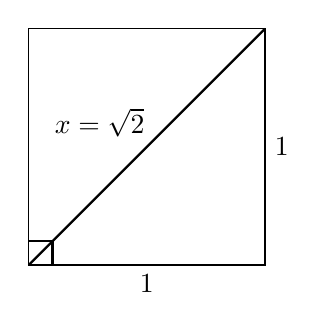
\begin{tikzpicture}[scale=3]
    \draw (0,0) -- (1,0) -- (1,1) -- (0,1) -- cycle;
    \draw[thick] (0,0) -- (1,1);
    \node[below] at (0.5,0) {$1$};
    \node[right] at (1,0.5) {$1$};
    \node[above, sloped] at (0.3,0.5) {$x = \sqrt{2}$};
    \draw[thick] (0.1,0) -- (0.1,0.1) -- (0,0.1);
  \end{tikzpicture}
  \caption{A square with side of 1 and its diagonal}
  \label{fig:square-diagonal}
\end{figure}

This theorem was list as Proposition 117 in Book X of \emph{The Elements}; after comparing with the old version, it turns out to be added by someone later. The latest version excluded it again. Consider a square with side of 1 and its diagonal (\cref{fig:square-diagonal}). Let the length of the diagonal be $x$; by Pythagorean theorem, $x^2 = 1^2 + 1^2 = 2$, denoted by $x = \sqrt{2}$. We give two proofs; the first was attributed to Pythagoras.

\begin{proof}
Assume by contradiction that $x$ equals some irreducible fraction $\dfrac{a}{b}$, where $a, b$ are coprime and $b \ne 1$.

\begin{align*}
2 &= x^2 = (\frac{a}{b})^2  && \text{by Pythagorean theorem} \\
a^2 &= 2b^2  && \text{multiply both sides by }b^2
\end{align*}

It implies $a^2$ is even, so is $a$ even. Let $a = 2c$ and substitute it:

\begin{align*}
(2c)^2 &= 2b^2 \\
2c^2 &= b^2 && \text{both sides divided by }2
\end{align*}

It follows $b^2$ is even, so is $b$; but $a, b$ are coprime, a contradiction. Thereby, $x = \sqrt{2}$ can not be irreducible fraction but irrational.
\end{proof}

The second proof, which is more generic, is the key to find more irrationals.
\begin{proof}
by $a^2 = 2b^2$ and $a, b$ are coprime, $b$ divides $a^2$. Since $b \ne 1$, any prime factor $p$ of $b$ also divides $a^2$. As $p$ is prime, it also divides $a$, it follows that $p$ divides both $a$ and $b$, which contradicts that $a, b$ are coprime.
\end{proof}

Essentially, Pythagoras's proof is a special case of $p = 2$ of the second proof. The generic method leads to a stronger theorem.

\begin{theorem}
If $n$ is not $m$-th power of some number, then $\sqrt[m]{n}$ is irrational.
\end{theorem}

\begin{proof}
Assume for contradiction that $\sqrt[m]{n} = \dfrac{a}{b}$ is some irreducible fraction, where $a, b$ are coprime and $b \ne 1$. Take the $m$-th power of both sides:
\[
a^m = n b^m
\]
It implies $b$ divides $a^m$, hence, any prime factor $p$ of $b$ also divides $a^m$. As $p$ is prime, it also divides $a$, it follows that $p$ divides both $a$ and $b$, which contradicts that $a, b$ are coprime.
\end{proof}

\index{straight edge and compass construction}
When $n$ is not a square number, as a special case of this theorem, then $\sqrt{n}$ is irrational. In this way, the Greeks discovered irrational geometric magnitude. When talking about geometric construction in Greece, it actually means the construction only with ruler and compass. According to the tradition of Plato, the ruler was unmarked, which was rather a straight edge. Different from the compass we used today, the two legs closed naturally due to gravity when lifted off the plan in ancient times. It was said the geometric construction with ruler and compass derived from the rope-meter in Egypt. Stretching the rope tight into a straight line, it derived to the ruler; Fixing one end and moving the other end of the rope, it derived to the compass. The Greeks insisted on challenging drawing all shapes only with such simple instruments and strict rules, from where Euclidean geometry flourished. \Cref{fig:euclid-soa} is part of \emph{School of Athens} by Raphael, a great artist in Renaissance. It shows Euclid drawing with a compass.

\begin{figure}[htbp]
 \centering
 \includegraphics[scale=0.35]{img/euclid-soa}
 \caption{Part of \emph{School of Athens}, fresco by Raphael, in the Stanza della Segnatura in the Vatican.}
 \label{fig:euclid-soa}
\end{figure}

Euclid postulated geometry constructions in the beginning of \emph{The Elements}:
\begin{enumerate}[{Postulate} (1)]
\item To draw a straight line from any point to any point. (ruler)
\item To produce a finite straight line continuously in a straight line. (ruler)
\item To describe a circle with any center and radius. (compass)
\end{enumerate}

Started from $\sqrt{2}$, the Greeks were able to construct a family of irrational numbers through the Pythagorean theorem. Given a line segment $AB$, let its length be 1, one may obtain a segment of length $n$ by copying $AB$ for $n$ times. Next draw a perpendicular line at one end (see \cref{qn:perp-of-point}), and then copy $AB$ for $m$ times. Finally connect the two ends of the perpendicular segment to form a right triangle. By the Pythagorean theorem, the length of the hypotenuse is $\sqrt{n^2 + m^2}$ (see \cref{fig:rt-mn}). When $m = n = 1$, the length is $\sqrt{2}$; when $m=1, n=2$, the length is $\sqrt{5}$.

\begin{figure}[htbp]
  \centering
  \subcaptionbox{The right triangle with the two sides of $n$ and $m$. \label{fig:rt-mn}}{
    \begin{tikzpicture}[scale=0.8]
      \draw (0,0) -- (7,0) -- (0,4) -- cycle;
      \node[below] at (3.5,0) {$n$};
      \node[left]  at (0,2) {$m$};
      \node[above, sloped] at (3.5,2.5) {$\sqrt{m^2 + n^2}$};
      \draw[thick] (0.1,0) -- (0.1,0.1) -- (0,0.1);
    \end{tikzpicture}
  }\subcaptionbox{The right triangle with the two sides of 1 and 2. \label{fig:rt-12}}{
    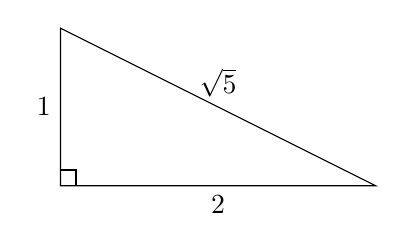
\begin{tikzpicture}[scale=2]
      \draw (0,0) -- (2,0) -- (0,1) -- cycle;
      \node[below] at (1,0) {$2$};
      \node[left]  at (0,0.5) {$1$};
      \node[above, sloped] at (1,0.5) {$\sqrt{5}$};
      \draw[thick] (0.1,0) -- (0.1,0.1) -- (0,0.1);
    \end{tikzpicture}
  }
  \caption{Irrational numbers obtained from the Pythagorean theorem.}
  \label{fig:irrational-tagent}
\end{figure}

\index{Golden ratio}
$\sqrt{5}$ is closely connected with a notorious number. Copy and append the unit segment (with length of 1) to make $1 + \sqrt{5}$, then halve it (see \cref{qn:perp-of-point}) to get $\phi = \frac{1 + \sqrt{5}}{2}$. This is the \emph{golden ratio}, its value\footnote{some uses 0.618, the approximate value of $\frac{\sqrt{5} - 1}{2}$ as the golden ratio. It can be obtained by first cutting off 1 from $\sqrt{5}$ followed by halving.} is approximately 1.618. \Cref{fig:gold-ratio} is the \emph{Vitruvian Man} by Leonardo da Vinci. It said he identified the golden ratio when studying the perfect human body, and intensely applied the golden ratio in his art works. Let the height of the Vitruvian man be 1, denote the section below waist by $x$, the section above waist by $1 - x$. da Vinci recognized the golden ratio of the two sections divided by waist, which was $(1 - x) : x$, equaled the ratio of the below section and the height of the body, which was $x : 1$. Written in equation as $(1 - x) : x = x : 1$. In fact, the golden ratio can be traced back to the ancient Greeks. Euclid, in \emph{The Elements}, called it, \enquote{extreme and mean ratio.} Change the equation to the identical of inner product and outer product (see \cref{sec:frac-equiv}), which gives: $x^2 + x - 1 = 0$; the two solutions of this quadratic equation are $x_{1, 2} = \frac{-1 \pm \sqrt{5}}{2}$.

\begin{figure}[htbp]
 \centering
 \includegraphics[scale=0.4]{img/gold-ratio}
 \caption{Vitruvian Man by Leonardo da Vinci, 1490}
 \label{fig:gold-ratio}
\end{figure}

By \cref{fig:gold-ratio}, $x < 1$, hence, $x = \frac{\sqrt{5} - 1}{2} \approx 0.618$. If let the section above the waist be 1, the section below the waist be $x$, then the golden ration, which divides the height of the body, is $1 : x$; it equal the ratio of the section below the waist and the height of the body, which is $x : (1 + x)$. Written in equation $1 : x = x : (1 + x)$, or in quadratic form of $x^2 - x - 1 = 0$. The two solutions are: $x_{1, 2} = \frac{1 \pm \sqrt{5}}{2}$. As $x > 0$, hence, $x = \frac{1 + \sqrt{5}}{2} \approx 1.618$. It turns out the two values are reciprocal of each other:

\[
\frac{\sqrt{5} - 1}{2} \times \frac{\sqrt{5} + 1}{2} = \frac{(\sqrt{5})^2 - 1}{4} = \frac{5 - 1}{4} = 1
\]

This is the reason that both $\phi = \frac{\sqrt{5} \pm 1}{2}$ are values of golden ratio depends on the context as shown in \cref{fig:2-cases-phi}. We next show either value of the golden ratio is irrational.

\begin{figure}
  \centering
  \subcaptionbox{$\phi = \frac{\sqrt{5} - 1}{2} \approx 0.618$}{
    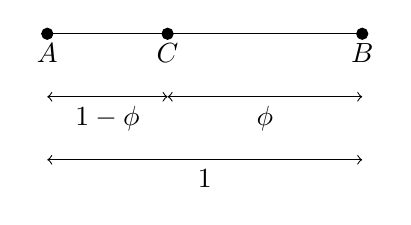
\begin{tikzpicture}[scale=4]
        \pgfmathsetmacro{\a}{0.382}

        \draw (0,0) -- (1,0);

        \filldraw (0,0) circle (0.5pt) node[below] {$A$};
        \filldraw (\a,0) circle (0.5pt) node[below] {$C$};
        \filldraw (1,0) circle (0.5pt) node[below] {$B$};

        \draw[<->] (0,-0.2) -- (\a,-0.2) node[midway,below] {$1-\phi$};
        \draw[<->] (\a,-0.2) -- (1,-0.2) node[midway,below] {$\phi$};
        \draw[<->] (0,-0.4) -- (1,-0.4) node[midway,below] {$1$};
    \end{tikzpicture}
  }\subcaptionbox{$\phi = \frac{\sqrt{5} + 1}{2} \approx 1.618$}{
    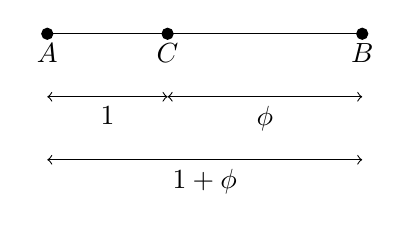
\begin{tikzpicture}[scale=4]
        \pgfmathsetmacro{\a}{0.382}

        \draw (0,0) -- (1,0);

        \filldraw (0,0) circle (0.5pt) node[below] {$A$};
        \filldraw (\a,0) circle (0.5pt) node[below] {$C$};
        \filldraw (1,0) circle (0.5pt) node[below] {$B$};

        \draw[<->] (0,-0.2) -- (\a,-0.2) node[midway,below] {$1$};
        \draw[<->] (\a,-0.2) -- (1,-0.2) node[midway,below] {$\phi$};
        \draw[<->] (0,-0.4) -- (1,-0.4) node[midway,below] {$1 + \phi$};
    \end{tikzpicture}
  }
  \caption{Two values of the golden ratio}
  \label{fig:2-cases-phi}
\end{figure}


\begin{proof}
Assume for contradiction that the golden ratio is rational, hence equals some irreducible fraction $\phi = \dfrac{a}{b}$, where $b \ne 1$. Substitute $\dfrac{a}{b}$ into the equation $\phi^2 \pm \phi - 1 = 0$,

\begin{align*}
(\frac{a}{b})^2 & = 1 \pm \frac{a}{b}  \\
a^2 &= b^2 \pm ab && \text{multiply both sides by }b^2 \\
a^2 &= b(b \pm a)
\end{align*}
Because $a, b$ are coprime, they can not be both even. Suppose $a$ is odd and $b$ is even, then $a^2$ on the left is odd, but the right side is even, a contradiction; If $a$ is even and $b$ is odd, then $a^2$ on the left is even, but $b \pm a$ on the right is odd; multiply by $b$, which is odd, gives odd again. It also leads to contradiction. If both $a, b$ are odd, the $a^2$ on the left is odd, but $b \pm a$ on the right is even, the product on the right is even. All three cases lead to contradiction, hence the golden ratio is irrational.
\end{proof}

In the second version of Hipassus's legend, the irrational number arose from the pentagram, the Pythagorean badge and liaison symbol. It happens this irrational number is the golden ratio $\phi$. Paul Lockhart shows this amazing connection in his book \emph{Measurement}.

\begin{figure}[htbp]
 \centering
 \includegraphics[scale=0.3]{img/pentagon}
 \caption{Regular pentagon}
 \label{fig:pentagon}
\end{figure}

\label{sec:pentagon-edge}
We divide the regular pentagon as \cref{fig:pentagon}. The isosceles triangle 1 and 2 are congruent, while 2 and 3 are similar (we skip the proof; roughly speaking, isosceles triangle 1 and 2 share a side and their base angles are both $36\degree$; isosceles triangle 2 and 3 have a pair of vertical angles). For the regular pentagon, let the length of the diagonal $BE$ be 1 and the length of the side be $x$. Since triangle 1 and 3 are similar,

\begin{align*}
\frac{x}{1} &= \frac{AB}{BE} = \frac{FC}{CD} && \text{1 and 3 are similar} \\
            &= \frac{EC - EF}{CD} = \frac{BE - AB}{CD} && BEC\text{ is isosceles, 1 and 2 are congurent} \\
            &= \frac{1-x}{x}
\end{align*}

It leads to the equation of $x^2 + x - 1 = 0$, to which the solution is the golden ration: $\phi = \frac{\sqrt{5} - 1}{2}$. For the Pythagorean badge, if the diagonal of the pentagram is 1, then the distance between two adjacent vertices is $\phi$, the side length of each angle is $1 - \phi$.

\index{Fibonacci sequence} \label{sec:Fibonacci-numbers}
The interest in golden ratio was revived from Renaissance. It has been mystified and became such a popular number, that may sayings or even rumors arose. It was said many ancient Greek and Roman arts and architectures employed the golden ratio, the most iconic example being the Parthenon in Athens. Leonardo da Vinci's work, such as the \emph{Mona Lisa} and \emph{The Virgin and Child with Saint Anne}, were all said to conform to the golden ratio. A rectangle whose length-to-width ratio equals the golden ratio is claimed to be the most beautiful of all rectangles, so much so that photographs, paper, and books are said to adopt dimensions based on the golden ratio. Some even assert that the golden ratio is hidden in all things in nature: the shell of the nautilus grows according to the golden ratio, and the seeds of a sunflower, the leaves of plants, and the inflorescences of broccoli all conform to it. These various claims have become increasingly mystical as they have spread, even appearing in novels and films (such as \emph{The Da Vinci Code}). It was Fibonacci, again, who gave us a tool to explain these phenomenon. He gave a well known problem in \emph{Liber Abaci}. Given a pair of newly born rabbits, one mail and one female; they are able to mate after one month and produce another pair of rabbits by the second month. Suppose rabbits never die and a mating pair always produces a new pair, one male and one female, every month. How many pairs will be there in one year?

In the first month, there is a pair; in the second month, plus the newly born pair, there are two pairs; in the third month, the matured pair produces another pair, while the pair born in the previous months are still young, in total 2 + 1 = 3 pairs; in the fourth month, the two matured pairs produce another two baby pairs, plus the three pairs in the third month, in total 3 + 2 = 5 pairs (see \cref{fig:Fibonacci-rabbits}). It results in a sequence of numbers,

1, 1, 2, 3, 5, 8, 13, 21, 34, 55, 89, 144, ...

\begin{figure}[htbp]
 \centering
 \subcaptionbox{The sides of squares form a Fibonacci sequence.\label{fig:fibonacci-spiral}}[0.45\linewidth]{
     \includegraphics[scale=0.4]{img/fibonacci_spiral}}
 \subcaptionbox{black: mature; white: newly born\label{fig:Fibonacci-rabbits}}[0.45\linewidth]{
     \includegraphics[scale=0.4]{img/Fibonacci-rabbits}}
 %\captionsetup{labelformat=empty}
 \caption{Fibonacci sequence interpretation}
\end{figure}

This sequence is called Fibonacci sequence, named after Fibonacci. It follows an obvious pattern: from the third one, every number is the sum of the previous two. We may understand its reason like this: suppose there are $n$ pairs of rabbits in some month and $m$ pairs in its previous month. The difference, which is $n - m$ pairs, are all newly born baby rabbits, while the remaining $m$ pairs are matured. In the next month, the $n - m$ pairs grow, and the $m$ matured pairs produces another $m$ pairs of baby rabbits. Hence the sum of matured pairs and baby pairs is $(n - m) + m + m = n + m$. It gives the recursive definition of Fibonacci sequence:

\begin{lalign}
F_0 &= 0 \\
F_1 &= 1 \\
F_{n+2} &= F_n + F_{n+1}
\end{lalign}

\index{Fibonacci spiral}
Fibonacci sequence starts from 0 and 1\footnote{When start from 1 and 3, one get Lucas sequence: $1, 3, 4, 7, 11, 18, \cdots$}. \Cref{fig:fibonacci-spiral} interprets Fibonacci sequence with a spiral. Start from two unit squares (side length of 1), form a rectangle with width of 1 and length of 1 + 1 = 2; Next put this $1 \times 2$ rectangle and a $2 \times 2$ square together to form a bigger rectangle with width of 2 and length of 2 + 1 = 3. Next put this $2 \times 3$ rectangle and a $3 \times 3$ square to form a rectangle of $3 \times 5$ and repeat. At any step, put a rectangle of $F_{n-2} \times F_{n-1}$ and a square $F_{n-1} \times F_{n-1}$ together to form a bigger rectangle with width of $F_{n - 1}$ and length of $F_n = F_{n-1} + F_{n-2}$. Inscribe every square with a 1/4 arc, these arcs form a Fibonacci spiral.

Fibonacci sequence grows very fast, the rabbits reproduce \emph{almost} exponentially, from a pair to 144 pairs in one year. We know geometric series increases exponentially as the ratio of any two consecutive numbers is fixed. What does the term `almost exponentially' mean? The proportions of two consecutive Fibonacci numbers are different as shown in \cref{tab:fibonacci-ratios}.

\begin{table}[ht]
    \centering
    \begin{tabular}{|c|c|l||c|c|l|}
        \hline
        $n$ & $F_n$ & $F_n/F_{n-1}$ & $n$ & $F_n$ & $F_n/F_{n-1}$\\
        \hline
        2 & 1 & 1 &         11 & 89   & 1.6181818182 \\
        3 & 2 & 2 &        12 & 144  & 1.6179775281 \\
        4 & 3 & 1.5 &        13 & 233  & 1.6180555556 \\
        5 & 5     & 1.667 &        14 & 377  & 1.6180257511 \\
        6 & 8     & 1.6 &         15 & 610  & 1.6180371353 \\
        7 & 13    & 1.625 &         16 & 987  & 1.6180327869 \\
        8 & 21    & 1.6153846154 &        17 & 1597 & 1.6180344478 \\
        9 & 34    & 1.6190476190 &        18 & 2584 & 1.6180338134 \\
        10 & 55   & 1.6176470588 &        19 & 4181 & 1.6180340557 \\
           &      &              &        20 & 6765 & 1.6180339632 \\
        \hline
    \end{tabular}
    \caption{Proportions of consecutive Fibonacci numbers}
    \label{tab:fibonacci-ratios}
\end{table}

Tough Fibonacci sequence is not a geometric series, as $n$ increases, the proportions of consecutive numbers are closing to a fixed value, which approximates to 1.6180 in four places. Calculate the golden ratio, with a calculator, $\phi = \frac{1+\sqrt{5}}{2} \approx 1.6180339887$, which matches $F_{20}/F_{19}$ for 7 places. Is that merely a coincidence?

\begin{proposition}
If the proportions of consecutive Fibonacci numbers converge, then the limit is the golden ratio $\phi$.
\end{proposition}

Note this proposition does not assert the existence of limit, but \emph{if} exits, then it is $\phi$. Despite we need analysis to show the limit exits, school math is sufficient for demystifying.

\begin{proof}
By the recursive definition of Fibonacci sequence: $F_n = F_{n-1} + F_{n-2}$, divide both sides by $F_{n-1}$,

\[
\frac{F_n}{F_{n-1}} = 1 + \frac{F_{n-2}}{F_{n-1}}
\]

If the proportions of consecutive Fibonacci numbers converge to $x$, which means when $n$ is increasing $n \to \infty$, both $\frac{F_n}{F_{n-1}}$ and $\frac{F_{n-1}}{F_{n-2}}$ converge to $x$, then the above equation turns out to be:

\begin{align*}
x = 1 + \frac{1}{x}  \\
x^2 - x + 1 = 0 && \text{multiply both sides by }x
\end{align*}
Which is exactly the equation of golden ratio. After discard the negative root, the solution is $x = \frac{\sqrt{5} + 1}{2} = \phi$.
\end{proof}

With a bit rational reasoning, we are able to explain why the golden ratio arises from many living things in nature: when something grows on top of its base but not reset, it follows the Fibonacci sequence. For example, a nautilus shell in its $n$-th growing cycle, grows on its base part of $F_{n-1}$ but not reset. Suppose it grows to $F_n$, then in the next cycle, it will grow based on $F_{n-1}$ and $F_n$ to $F_{n+1} = F_{n} + F_{n-1}$. It grows exactly by following the recursive relation of Fibonacci sequence as shown in \cref{fig:fibonacci-spiral}, a Fibonacci spiral. This spiral inscribes a rectangle whose length-to-width ratio is $F_{n}/F_{n-1}$, which converges to the golden ratio. In the same way as shown in \cref{fig:sunflower}, the sunflower grows on its base but not reset, hence the numbers of seeds become a Fibonacci sequence. Its growing pattern forms a Fibonacci spiral, which inscribes rectangles whose dimension close to the golden ratio. This pattern is so common in nature, that it explains why leaves, flowers, seeds, shells, and so on, all describe Fibonacci numbers, hence describe the golden ratio.

\begin{figure}[htbp]
 \centering
 \includegraphics[scale=0.3]{img/sunflower}
 \caption{Seeds of a sunflower follow Fibonacci sequence.}
 \label{fig:sunflower}
\end{figure}

The next rumor to be clarified is about paper size, which is said to adopt golden ratio because such rectangles look most beautiful. \Cref{fig:ISO216} shows the definition of International Standards Organization (ISO) paper size of A series and B series, annotated in both mm and in. The commonly used A4 paper for example, is $210 \times 297 mm^2$; its length-to-width ratio is $297/210 = 1.41429$, unequal to the golden ration of 1.618. The ratio of B0 paper is $1414/1000 = 1.414$. It looks that the length-to-width ratio of these papers are close. While 1.414 is near $\sqrt{2}$, the diagonal length of a unit square and the notorious irrational number discovered by the ancient Greeks. Is that a coincidence? According to the explanation of ISO, a piece of A0 paper covers area of $1 m^2$; a piece of A0 paper can be divided into two pieces of A1 paper, in the same shape of rectangle; a piece of A1 paper can be divided into two pieces of A2 paper in the same shape of rectangle, and so on. Similarly, a piece of B0 paper can be divided into two pieces of B1; a piece of B1 can be divided into two pieces of B2, and so on. The meaning of same shape, by school math, is \emph{similar} rectangle for both A series and B series. To figure out what length-to-width ratio satisfying such dividing rule, let the length be $r$ and the width be $1$ (B0 for example); divide it into two pieces of small paper (B1 for example) with length of $1$ and width of $\dfrac{r}{2}$. Since they are similar,

\begin{figure}[htbp]
 \centering
 \includegraphics[scale=0.25]{img/ISO216}
 \caption{ISO A series and B series.}
 \label{fig:ISO216}
\end{figure}

\begin{align*}
r : 1 &= 1 : \frac{r}{2}  && \text{Similar} \\
1 &= \frac{r^2}{2} && \text{inner product equals outer product} \\
r^2 &= 2
\end{align*}

Therefor, $r = \sqrt{2}$. It explains why the length-to-width ratio of ISO papers equals $\sqrt{2}$. Since irrational, it is non-repeating decimal, hence there is precision loss after rounding or unit changing. For example, the ratio of $B5$ is $250/176 = 1.42$. One may figure out the size of A0 by himself: since A0 covers $1 m^2$, let the width be $a$, the length be $a\sqrt{2}$; the area $s = a^2\sqrt{2} = 1$. Solving this equation gives $a = \sqrt{\frac{1}{\sqrt{2}}} \approx 0.841 m$. Hence the length is $1 / 0.841 = 1.189 m$, which is exactly as same as \cref{fig:ISO216}. At the same time, one may deduce the definition of B series: a B0 paper covers area of $\sqrt{2} m^2$. Each size of $B$ series is $\sqrt{2}$ times to the size of A series. We can further reason out that, when manufacturing rectangular bricks or tiles, to make them easy cutting to similar pieces, the length-to-width ratio must be $\sqrt{2}$. In this way, we demystified and clarified the rumors with rationality and mathematics. Some may think its dull, not romantic at all. While, the reasoning process itself is beautiful, reveals the theories and rules of nature and human activities. Aren't these theories and rules harmonic, beautiful, and romantic?

\index{Luogeng Hua} \index{optimization method}
We end this section with `the last lecture' of Chinese mathematician, Luogeng Hua\footnote{Hua died of a heart attack at the end of this lecture he gave in Tokyo on 12 June 1985 at the age of 74. The lecture was titled \emph{Theory, application, and its popularization}. After the lecture, Hua walked towards his wheelchair in applause, but unfortunately collapsed to the ground. He died at 10 PM that same night\citepage[p21]{ZhangJianan-2017}.}.

\begin{quotation}
When taught the optimization method in a factory, it would be impossible to require all workers had studied calculus. So how did I popularize optimization methods in China? First of all, I asked everyone to remember a number: 0.618. This slip of paper and this cigarette are my teaching aids. Let’s assume the slip of paper represents the range of some factor. Where should the first experiment be conducted? At the position of 0.618 along the entire length. (Hua lit the cigarette and burned a hole in the slip of paper at the 0.618 mark.) Where should the second experimental be conducted? At the point symmetric to the first, which I can find very simply here. Fold the paper in half and burn through the hole made by the first experimental point — then you get the second experimental point. At this time, you can compare the results obtained from the two experiments and see which one is better. If the first is better, then tear off the part below the second point; otherwise tear off the part above the first point. Where should the next experiment be conducted? Again, fold the remaining slip in half and burn through the remaining hole from the previous experiment, and you will get the third experimental point. Then compare again, keep the better one, and tear off the worse one. I don’t need to explain what to do next, right? (Laughter) Continue this process until the precision required in production is achieved.
\end{quotation}

\section{Euclidean algorithm}
\label{sec:Euclidean-algorithm}

The Greeks identified the newly discovered numbers different from other numbers. First, they did exist since one can construct such magnitudes with ruler and compass. Second, they were not whole number or ratio of whole numbers. In order to treat them as numbers, there are several problems to be answered: (1) How to define them? (2) How to `measure' their magnitude? (3) Where are they one the number line? (4) Though they are not irreducible fractions, can we approximate them with fractions? These questions lead to fruitful result in the hand of Eudoxus.

We mentioned in geometric construction, first define a given line segment as 1, then one may extend (by taking with compass) it to $n$. The segment of 1 acts like a ruler, which is used to `measure' a segment of $n$. Explained in `all is number', the Pythagoreans raised the notion of measure: when the length of a line segment A, equals the total length of finite many line segments of V, then define V measures A. In other words, one duplicates a line segment integral times to form another segment. Two line segments $A$ and $B$ may have their own different measures, but if a segment $V$ measures $A$ and $B$, it must be their \emph{common measure}, that is $V$ measures $A$ and $V$ measures $B$. Thus `all is number' means there exists common measure for any two line segments.

\index{The greatest common measure}
There can be multiple common measures, so it makes sense to define the \emph{greatest} common measure\footnote{abbreviated as gcm. In the context of numbers but not line segments, the corresponding concept is the greatest common divisor, abbreviated as gcd.} as the greatest line segment $V$ that measures both $A$ and $B$, and is not less than any common measure of them. Given two line segments, how to find their greatest common measure? It was this problem that led to a famous algorithm in history: Euclidean algorithm\footnote{Euclidean algorithm was developed independently in other cultures, such as India and China. Indian mathematician Aryabhata applied this algorithm to solving Diophantine equations by the end of the 5th century. In a Chinese book \emph{The Mathematical Classic of Sunzi}, the corresponding Euclidean algorithm was treated as a special case of Chinese remainder theorem. In 1274 (the Southern Song Dynasty), mathematician Qiushao Qin gave a detailed account of Euclidean algorithm in his book \emph{The Mathematical Treatise in Nine Chapters}.}. This algorithm appears\footnote{There is another one, namely the Proposition 1 in Book VII, about Euclidean algorithm for integers. This one, which is for line segments, covers integers.} as Proposition 3, in Book X of Euclid's \emph{The Elements}.

\index{Euclidean algorithm}
\begin{proposition}[Proposition 3, Book X, The Elements]
To find the greatest common measure of two given commensurable magnitudes.
\end{proposition}

We brief the Euclidean algorithm in \cref{sec:gcd-minus} to compute the greatest common divisor of two natural numbers. In \emph{The Elements}, it was actually extended to geometric magnitudes, such as line segments, as a generic algorithm. The original algorithm given by Euclid only required recursive subtraction, hence could be implemented by ruler and compass. perfectly. Below is the definition:

\[
(a, b) = \begin{cases}
  a > b :& (a - b, b) \\
  a = b :& a \\
  a < b :& (a, b - a)
  \end{cases}
\]

Suppose line segment $a$ and $b$ are commensurable. If they have the same length, then the greatest common measure is either segment; the algorithm gives $a$ as the result. If $a$ is longer than $b$, we cut off $b$ from $a$ and repeat (through recursion), then recursively compute the greatest common measure of the remaining segment $a'$ and $b$; if $b$ is longer than $a$, then cut off $a$ from $b$ and repeat, then recursively compute the greatest common measure of $a$ and the remaining segment $b'$. \Cref{fig:line-seg-gcm} shows the steps when applying this algorithm to two line segments. We may also apply it to numbers 42 and 30 as,

\[
(42, 30) = (12, 30) = (12, 18) = (12, 6) = (6, 6) = 6
\]

\begin{figure}[htbp]
  \centering
  \begin{tikzpicture}[scale=0.125]
    \filldraw (0, 0) circle (0.5)   (30, 0) circle (0.5)   (42, 0) circle (0.5);
    \draw (-8, 0) node{$a$} (0, 0) -- (42, 0);
    \filldraw (0, -5) circle (0.5)   (30, -5) circle (0.5);
    \draw (-8, -5) node{$b$} (0, -5) -- (30, -5);

    \filldraw (0,  -15) circle (0.5)   (12, -15) circle (0.5);
    \draw (-8, -15) node{$a'=a-b$} (0, -15) -- (12, -15);
    \filldraw (0, -20) circle (0.5)   (12, -20) circle (0.5)   (24, -20) circle (0.5)   (30, -20) circle (0.5);
    \draw (-8, -20) node{$b$} (0, -20) -- (30, -20);

    \filldraw (0,  -30) circle (0.5)   (6, -30) circle (0.5)   (12, -30) circle (0.5);
    \draw (-8, -30) node{$a'$} (0, -30) -- (12, -30);
    \filldraw (0, -35) circle (0.5)   (6, -35) circle (0.5);
    \draw (-8, -35) node{$b'=b-2a'$} (0, -35) -- (6, -35);

    \filldraw (0,  -45) circle (0.5)   (6, -45) circle (0.5);
    \draw (-8, -45) node{$a''=a'-b'$} (0, -45) -- (6, -45);
    \filldraw (0, -50) circle (0.5)   (6, -50) circle (0.5);
    \draw (-8, -50) node{$b'$} (0, -50) -- (6, -50);
  \end{tikzpicture}
  \caption{Steps of Euclidean algorithm.}
  \label{fig:line-seg-gcm}
\end{figure}

\subsection{Improved Euclidean algorithm} \index{division algorithm}
The operation of subtracting $b$ from $a$ and repeating to get $a'$, by definition, is exactly the division algorithm: $a' = a - qb$, where $q$ is the quotient and $a'$ is the remainder. Gauss introduced a notation, namely $a'= a \bmod b$, with which we may simplify the repeat of segment cutting (by compass) in Euclidean algorithm. When a magnitude is some multiple of the other, for example, $b \leq a$ and $b$ divides $a$, we immediately know the greatest common measure is $b$. Since the remainder, $a \bmod b = 0$, we define $(0, b) = (b, 0) = b$. Before applying Euclidean algorithm, we may firstly compare $a$ and $b$, if $a < b$, then swap them. Since $a \bmod b$ must be less than $b$, we swap before recursively computing $(b, a \bmod b)$. Below definition summarizes these improvement.

\be
(a, b) = \begin{cases}
  a < b: & (b, a) \\
  b = 0: & a \\
  a > b: & (b, a \bmod b)
\end{cases}
\label{eq:gcm}
\ee

\begin{proof}
We take two steps to show why this algorithm gives the greatest common measure: (1) show this algorithm gives a common measure; (2) show it is the greatest. Suppose $b \leq a$, otherwise swap them. Apply the division algorithm to $a$ and $b$; let $q_0$ be the quotient (a integer, which is the number of times that cutting $b$ from $a$ by compass), $r_0$ be the remainder (the remaining segment), such that $a = b q_0 + r_0$. If $r_0 = 0$, then $b$ is the common measure (segment $b$ measures $a$ perfectly); we only need consider the case of $r_0 \ne 0$. Apply the division algorithm again: $b = r_0 q_1 + r_1$; as far as the remainder isn't zero, we get a list like below:

\begin{align*}
a   &= b q_0 + r_0 \\
b   &= r_0 q_1 + r_1 \\
r_0 &= r_1 q_2 + r_2 \\
r_1 &= r_2 q_3 + r_3 \\
    & \cdots
\end{align*}

The list can not be endless since $a$ and $b$ are commensurable. This is because the quotients are integral (the times of cutting off a segment by compass), and the remainders are always less than the divisors. For the chain of remainders: $b > r_0 > r_1 > r_2 > \dotsb \ge 0$, since the remainder can't be negative and the starting number is finite, it eventually reaches,

\begin{salign}
       & \cdots \\
r_{n-1} &= r_n q_{n+1}
\label{eq:termination-of-euclidean-algorithm}
\end{salign}

We are going to show $r_n$, in the last step, measures both $a$ and $b$. \Cref{eq:termination-of-euclidean-algorithm} implies $r_n$ measures $r_{n-1}$ by definition. By the second last equation $r_{n-2} = r_{n-1} q_n + r_n$, since $r_n$ measures $r_{n-1}$, $r_n$ also measures $r_{n-1} q_n$, hence it measures $r_{n-1} q_n + r_n$, which equals $r_{n-2}$. In the same way, $r_n$ measures $r_{n-1}, r_{n-2}, \dotsc, b, a$, thereby, $r_n$ is a common measure of $a$ and $b$.

Next we are going to show $r_n$ is the greatest common measurement; in other words, any common measure $c$ of $a$ and $b$ measures $r_n$. As $c$ is a common measure, both $a$ and $b$ are its multiples, let $a = mc, b = nc$, where $m, n$ are integral. Substitute into $a = b q_0 + r_0$, it gives $mc = ncq_0 + r_0$; turn it into $r_0 = (m - nq_0)c$, which shows $c$ measures $r_0$. In the same way, $c$ measures $a, b, r_0, r_1, \dotsc, r_n$. Thus any common measure $c$ also measures $r_n$, hence $r_n$ is the greatest common measure. This proves the Euclidean algorithm.
\end{proof}

We often use symbol $d = r_n$ for the greatest common measure of $a$ and $b$. Actually, $d$ is the greatest common measure of every pair below:

\be
d = (a, b) = (b, r_0) = \dotso = (r_{n-1}, r_n) = r_n
\label{eq:recursive-gcm}
\ee

\Cref{fig:geometric-GCM} gives another geometric interpretation on Euclidean algorithm. The greatest common measure of $a$ and $b$ corresponds to the biggest square tile that paves a rectangle with length of $a$ and width of $b$. Consider a piece of paper with size of $a \times b$, we first cut off squares with side of $b$; it remains a piece of paper with size of $b \times r_0$. Next cut off squares with side of $r_0$; it remains a piece of paper with size of $r_0 \times r_1$; cut off squares and repeat, the side of the finally remained square is the greatest common measure. We can pave the rectangle with tiles of such a square.

\begin{figure}[htbp]
 \centering
 \subcaptionbox{Cut off squares and repeats: (1) up left: rectangle of $b \times a$; (2) bottom left: cut off two squares with side of $a$; (3) up right: cut off three squares with side of $c$; (4) bottom right: cut off four squares with side of $d$.}{\includegraphics[scale=0.4]{img/GCM}}
 \subcaptionbox{Pave the rectangle with the biggest squares}{
   \begin{adjustbox}{max width=0.8\textwidth}
   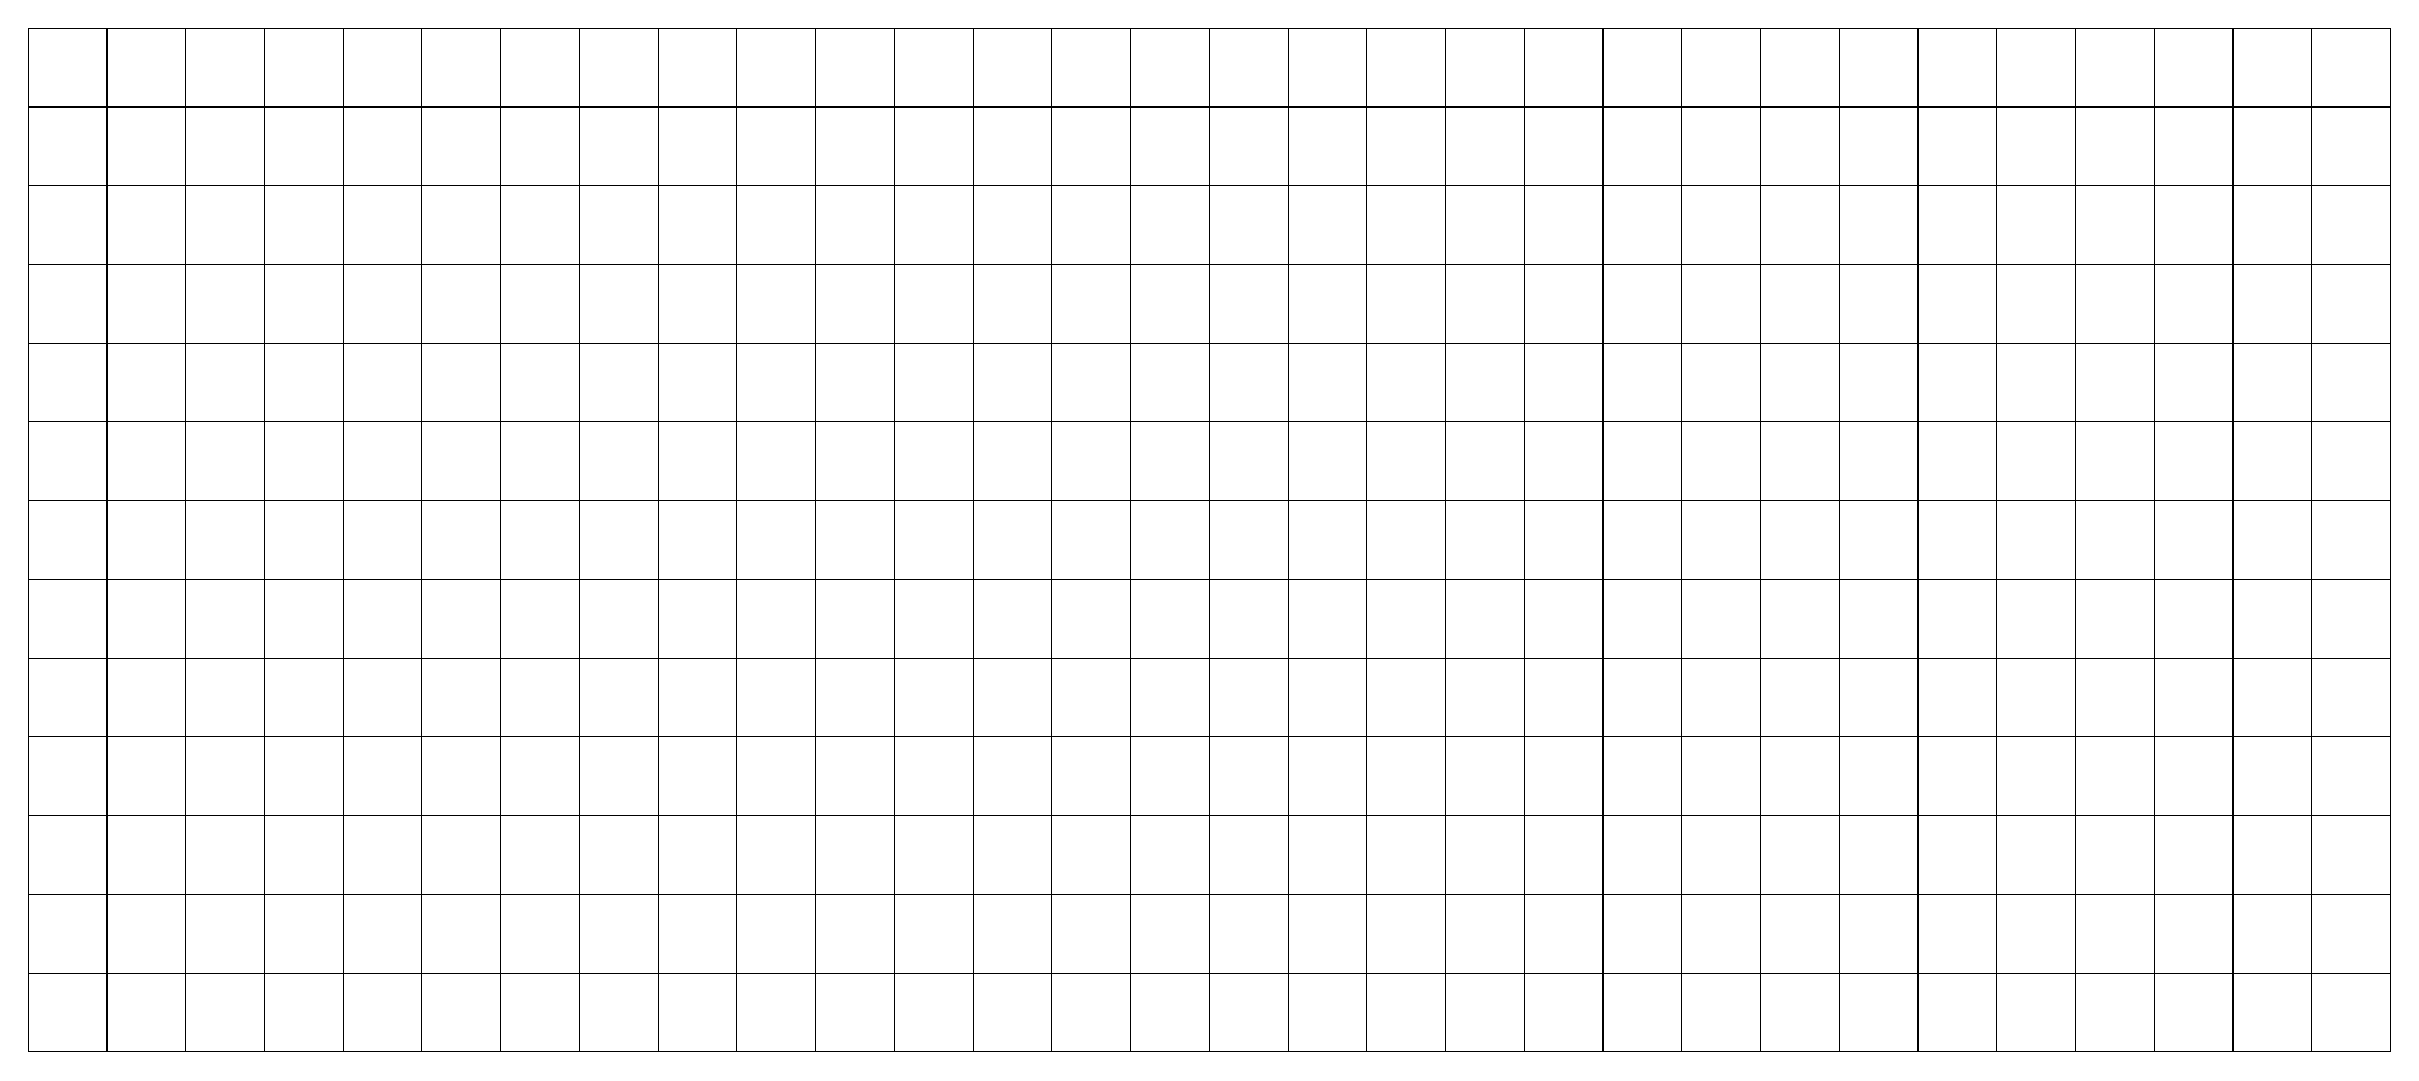
\begin{tikzpicture}
     \draw[step=1, thin] (0, 0) grid (30, 13);
   \end{tikzpicture}
   \end{adjustbox}
 }
 \caption{Geometric interpretation on Euclidean algorithm}
 \label{fig:geometric-GCM}
\end{figure}

\subsection{Extended Euclidean algorithm}
\index{Extended Euclidean algorithm} \index{Bézout's identity}

Bézout's identity is a direct result from Euclidean algorithm. Bachet (\cref{fig:Bachet}) was the first who proved this identity for integers. Bézout (\cref{fig:Bezout}) showed it was applicable to polynomials\footnote{In abstract algebra, Bézout's identity holds in any principal ideal domain (PID).}.

\begin{figure}[htbp]
 \centering
 \subcaptionbox{Étienne Bézout, 1730 - 1783 \label{fig:Bezout}}[0.45\linewidth]{\includegraphics[scale=0.45]{img/Bezout}}
 \subcaptionbox{Claude Gaspard Bachet de Méziriac, 1581 - 1638 )\label{fig:Bachet}}[0.45\linewidth]{\includegraphics[scale=0.95]{img/Meziriac}}
 \caption{Bézout and Bachet}
\end{figure}

\begin{theorem}[Bézout's identity]
For the greatest common measure $d$ of $a$ and $b$, there are integers $x$ and $y$ satisfying

\be
ax + by = d
\label{eq:bezouts-identity}
\ee
\end{theorem}

\begin{proof}
Consider the set of all positive magnitudes in the form of $ax + by$, namely,

\[
S = \{ ax + by \}, x, y \text{are integral, and } ax + by > 0
\]

$S$ is not empty as at least, it contains $a$ (for $x = 1, y = 0$) and $b$ ( for $x = 0, y = 1$). Since all elements of $S$ are positive, there exists the least one, denoted by $d = as + bt$. We are going to show $d$ is the greatest measure of $a$ and $b$. Apply the division algorithm to $a$ divided by $d$,

\be
a = qd + r
\label{eq:Euclidean-division}
\ee

Where $q$ is the quotient. Since the remainder $0 \leq r < d$, it follows that the remainder $r$ is either 0, or in $S$, because,

\begin{align*}
r & = a - qd          && \text{by \cref{eq:Euclidean-division}} \\
  & = a - q(as + bt)  && \text{substitute in }d = as + bt \\
  & = a(1 - qs) - bqt && \text{collect the terms} \\
  & = ax' + by'       && \text{let }x' = 1 - qs, y' = -bq
\end{align*}

which is in the form of elements contained in $S$. Remind we selected $d$ as the least positive element in $S$, but $r$ is less than $d$, a contradiction. Therefore, $r = 0$, \cref{eq:Euclidean-division} is then $a = qd$, which implies $d$ measures $a$. In the same way, $d$ also divides $b$. Hence $d$ is the common measure. Next, we shall show $d$ is the greatest common measure. For any common measure $c$ of $a$ and $b$, by definition, $a = mc$ and $b = nc$ for some integers $m$ and $n$. Substitute them in,

\begin{align*}
d & = as + bt    \\
  & = mcs + nct  && c\text{ is common measure of $a$ and $b$.} \\
  & = c(ms + nt) && d\text{ is multiple of $c$.}
\end{align*}

It follows that $c$ measures $d$, hence, $c \leq d$. As $c$ is an arbitrary common measure, thereby, $d$ is the greatest common measure. This proves Bézout's identity, i.e., there are integers $x$ and $y$ satisfying $ax + by = d$, and the greatest common measure is the smallest one among all the positive numbers of $ax + by$.
\end{proof}

How to find $x$ and $y$ such that $d = ax + by$? With Bézout's identity, we \emph{extend} the Euclidean algorithm, which will compute the greatest common measure and the corresponding $x$ and $y$:

\begin{align*}
ax + by & = d = (a, b)   && \text{by Bézout's identity} \\
        & = (b, r_0)     && \text{by Euclidean algorithm, \cref{eq:recursive-gcm}} \\
        & = bx' + r_0 y' && \text{Apply Bézout's identity to $b$ and $r_0$.} \\
        & = bx' + (a - bq_0)y'  && \text{by } a = b q_0 + r_0 \\
        & = ay' + b(x' - y'q_0) && \text{collect terms of $a$ and $b$} \\
        & = ay' + b(x' - y' \lfloor a / b \rfloor) && \text{$q_0$ as the quotient of }\lfloor a / b \rfloor
\end{align*}

This is a recursive relation of,

\[
x = y' \qquad y = x' - y' \lfloor a / b \rfloor
\]

The recursion terminates when $b = 0$, at this point, the greatest common measure is $(a, 0) = 1a + 0b$. We summarize these to the extended Euclidean algorithm:

\be
(a, b)' =
\begin{cases}
  a < b: & (b, a)' \\
  b = 0: & (a, 1, 0) \\
  a > b: & (d, y', x' - y' \lfloor a / b \rfloor), \text{where }(d, x', y') = (b, a \bmod b)'
\end{cases}
\label{eq:gcm-ext}
\ee

We use the notation of $(a, b)'$ to differentiate it from the original Euclidean algorithm; its result contains three parts: $(d, x, y)$, which are the greatest common measure and the corresponding $x$ and $y$. If $a < b$, then swap them; if $b = 0$, then $a$ is the greatest common measure and $x = 1, y = 0$, hence the result is $(a, 1, 0)$; otherwise, we recursively apply the extended Euclidean algorithm to compute $(b, a \bmod b)'$ for the greatest common measure $d$ and the corresponding $x'$ and $y'$, then by the recursive relation of $x = y', y = x' - y' \lfloor a / b \rfloor$, to obtain $x, y$.

For the same example of 42 and 30, apply the extended Euclidean algorithm: $(d, x, y) = (42, 30)'$,
\begin{enumerate}[{Step}(1)]
\item Recursively compute $(d, x', y') = (30, 12)'$, where 12 is the remainder of $42 \div 30$;
\item Recursively compute $(d, x'', y'') = (12, 6)'$, where 6 is the remainder of $30 \div 12$;
\item Recursively compute $(6, 0)'$, where 0 is the remainder of $12 \div 6$. By the termination case, $(6, 0)' = (6, 1, 0)$, hence, $(d = 6, x''' = 1, y''' = 0)$;
\item Return to (2), it gives $(d = 6, x'' = y''' = 0, y'' = x''' - \lfloor 12/6 \rfloor y''' = 1 - 2 \times 0 = 1)$;
\item Return to (1), it gives $(d = 6, x' = y'' = 1, y' = x'' - \lfloor 30/12 \rfloor y'' = 0 - 2 \times 1 = -2)$;
\item Finally return to get $(d = 6, x = y' = -2, y = x' - \lfloor 42/30 \rfloor y' = 1 - 1 \times (-2) = 3)$.
\end{enumerate}
It's easy to verify that $ax + by = 42 \times (-2) + 30 \times 3 = 6 = d$, indeed, it is the greatest common measure.

Here is an application of the Extended Euclidean algorithm for example, In a popular puzzle\citepage[p23]{LiuXinyu-2022}, given two jugs of 9 and 4 litres, how to get 6 litres of water from river? This puzzle has some variants and can be traced back to ancient Greeks. A story said French mathematician Sim\`{e}on Denis Poisson solved this puzzle when he was a child. Let the small jug be $A$ of capacity $a$, the big jug be $B$ of capacity $b$. There are 6 operations each time: (1) Fill jug $A$; (2) Fill jug $B$; (3) Empty jug $A$; (4) Empty jug $B$; (5) Pour from jug $A$ to $B$; (6) Pour from jug $B$ to $A$. The last two operations stop when either jug is full or empty. \Cref{tab:jug-ops} lists a series of operation for example (suppose $a < b < 2a$).

\begin{table}[htbp]
\centering
\begin{tabular}{|l|l|l|}
\hline
$A$ & $B$ & operation \\
\hline
0 & 0 & start \\
0 & $b$ & fill $B$ \\
$b$ & 0 & pour $B$ to $A$ \\
$b$ & $b$ & fill $B$ \\
$a$ & $2b - a$ & pour $B$ to $A$ \\
0 & $2b - a$ & empty $A$ \\
$2b - a$ & 0 & pour $B$ to $A$ \\
$2b - a$ & b & fill $B$ \\
a & $3b - 2a$ & pour $B$ to $A$ \\
... & ... & ... \\
\hline
\end{tabular}
\caption{The water in two jugs and operations}
\label{tab:jug-ops}
\end{table}

The key point is that, whatever operations, the water in each jug is $ax + by$ litres for some integral $x$ and $y$. We known from the proof of Bézout's identity, the least positive volume of water is the greatest common measure $d$ of $a$ and $b$. One is able to obtain $c$ litres of water if and only if $d$ measures\footnote{For integral capacities, if and only if the greatest common divisor $d$ divides $c$} $c$, and $c$ doesn't exceed the capacity of the bigger jug. For example, one can not get 5 litres of waters with two jugs of 4 litres and 6 litres, because the greatest common divisor of 4 and 6 is 2, which does not divide 5 (In other words, one can't get odd litres of water with two jugs of even litres capacity). If $a$ and $b$ are coprime, of which the greatest common divisor $(a, b) = 1$, then one is able to get any $c$ litres of water, where $c$ is a natural number is less than the capacity of the bigger jag.

Though one can tell if it's possible to get $c$ litres of water by examine the greatest common divisor $d$, he doesn't know the detailed steps. We may work out the steps from the two integers $x$ and $y$ satisfying $ax + by = c$ such that if $x > 0$ and $y < 0$, we fill $A$ for $x$times and empty $B$ for $y$ times; otherwise if $x < 0$, $y > 0$, then empty $A$ for $x$ times and fill $B$ for $y$ times. For example, suppose the bigger jug has capacity of $a=5$ litres, the smaller jug has capacity of $b=3$ litres, and the goal is to get $c=4$ litres of water; by $4 = 3 \times 3 - 5$, that is $x = -1$ and $y = 3$, design steps as \cref{tab:designed-jugs-ops}.

\begin{table}[htbp]
\centering
\begin{tabular}{l|l|l}
$A$ & $B$ & operation \\
\hline
0 & 0 & start \\
0 & 3 & fill $B$ \\
3 & 0 & pour $B$ to $A$ \\
3 & 3 & fill $B$ \\
5 & 1 & pour $B$ to $A$ \\
0 & 1 & empty $A$ \\
1 & 0 & pour $B$ to $A$ \\
1 & 3 & fill $B$ \\
4 & 0 & pour $B$ to $A$ \\
\end{tabular}
\caption{steps to get 4 litres of water} \label{tab:designed-jugs-ops}
\end{table}

In total, we fill $B$ for 3 times and empty $A$ once. The remaining is to find integers $x$ and $y$ such that $ax + by = c$. Applying the extended Euclidean algorithm, one gets a special solution to the Bézout's identity $ax_0 + by_0 = d$. Suppose $c$ is a multiple of the greatest common measure $d$ for $m$ times, multiply $x_0$ and $y_0$ by $m$ to get a solution of,

\[
\begin{dcases}
  x_1 = x_0 \dfrac{c}{d} \\
  y_1 = y_0 \dfrac{c}{d}
\end{dcases}
\]

\label{sec:linear-diophantus-equation} \index{linear Diophantine equation}
We then generate \emph{all} solutions from it to the Diophantine equation\footnote{Named after Diophantus of Alexandria (about 200-284 CE), who introduced algebraic notation and symbolism in his influential work \emph{Arithmetica}. Diophantus was known as \enquote{the father of algebra.}\cite{HanXueTao2009}.}:

\be
\begin{dcases}
  x = x_1 - k \dfrac{b}{d} \\
  y = y_1 + k \dfrac{a}{d}
\end{dcases}
\ee

Where $k$ is integral. For the puzzle of getting 6 litres of water from jugs of 9 and 4 litres, apply the extended Euclidean algorithm to the computation of $(9, 4)'$, which in turn to recursively compute $(4, 1)'$, then recursively compute $(1, 0)'$ to get $(d = 1, x''= 1, y'' = 0)$; return to give $(d = 1, x = 1, y = -2)$. Multiply it by 6 times, thereby, one need fill the jug of 9 litres for 6 times and empty the jug of 4 litres for 12 times. \Cref{qn:best-steps-water} ask to figure out the fewest steps.

\subsection{Euclidean algorithm and irrationals}

Euclidean algorithm applies to both integers and geometric magnitudes; the latter actually covers the former (when the length is integral). Contrary to what the Pythagoreans thought, geometry was not built on top of the idea of \enquote{all is number}, but was developed independently on the notion of numbers or ratios of numbers. The Greek in turn established a tradition, that all propositions, even about number, had to provide geometric argument. It influenced people deeply, that in the 16th century, when the Italian mathematician Cardano published solutions to the cubic and quartic equations, he gave geometric argument in \emph{Ars Magna}\cite{HanXueTao2009} (see \cref{sec:geometric-cubic-solution}). However, the Euclidean algorithm, as a double-sided sword, attack back to the Pythagoreans's belief, \enquote{all is number}, that all numbers are commensurable. Applying the Euclidean algorithm to the side and diagonal of a square,

\begin{proposition}
The side and diagonal of a square are not commensurable.
\end{proposition}

\begin{figure}[htbp]
 \centering
 \includegraphics[scale=1.5]{img/irrational}
 \caption{Side and diagonal of a square}
 \label{fig:irrational}
\end{figure}

\begin{proof}
In the 19th century, Scottish mathematician George Chrystal reconstructed the Greek proof. Assume for contradiction there exists some segment $c$ that measures the side and diagonal of a square, let the side be $nc$ and the diagonal be $mc$, where $m$ and $n$ are natural numbers. As shown in \cref{fig:irrational}, taking the side as radius, draw an arc around $A$ as the center, which intersects the diagonal $AC$ at point $E$. Then draw a line from $E$ perpendicular to the diagonal and intersects side $BC$ at point $F$.

For arc, the length of $AE$ equals the square side, hence the length of EC equals $(m - n)c$. Since EF is perpendicular to AC and $\angle ECF$ is $45\degree$, ECF is a isosceles right triangle; the two sides $|EC| = |EF|$. The two right triangles, $\triangle AEF$ and $\triangle ABF$ are congruent because they share a side of $AF$ and AE equals AB. Thereby, $|EF| = |FB|$, it follows that $|EC| = |EF| = |FB|$, so the length of FB equals $(m - n)c$ too. The length of CF which is CB minus FB, equals $nc - (m - n)c = (2n - m)c$. We list them side by side as below.

\[
\begin{array}{c|c}
\begin{cases}
|AC| = mc \\
|AB| = nc
\end{cases} &
\begin{cases}
|CF| = (2n - m)c \\
|CE| = (m - n)c
\end{cases} \\[4ex]
\text{big square} & \text{small square}
\end{array}
\]

As $m$ and $n$ are natural numbers, and $c$ measures diagonal $CF$ and side $CE$. In the same way, we can construct smaller and smaller squares and repeat infinitely, while $c$ measures the side and diagonal of each small square. Since $m$ and $n$ are finite natural numbers, the process can't be endless, a contradiction. Therefore, the side and diagonal of a square are not commensurable.
\end{proof}

Analog to square, \cref{qn:pentagon-irrational} requires to show the side and diagonal of a pentagon are not commensurable. In this way, Euclid gave the criterion of differentiate rationals and irrationals: whether Euclidean algorithm terminates. He also used this criterion to define rational magnitude and irrational magnitude.

\index{incommensurable}
\begin{proposition}[Proposition 2, Book X, The Elements] \label{th:irrational-gcm}
If, when the less of two unequal magnitudes is continually subtracted in turn from the greater that which is left never measures the one before it, then the two magnitudes are incommensurable.
\end{proposition}

\begin{definition}[Definition 3, Book X, The Elements]
... with an assigned straight line. Let then the assigned straight line be called rational, and those straight lines which are commensurable with it, whether in length and in square, or in square only, \emph{rational}, but those that are incommensurable with it \emph{irrational}.
\end{definition}

\subsection{Applications of Euclidean algorithm}

\index{RSA algorithm}
Euclidean algorithm has many applications. \Cref{sec:linear-diophantus-equation} shows how to apply Euclidean algorithm to the linear Diophantine equation of $ax + by = c$, firstly, figure out the greatest measurement $d$, and test whether $d$ divides $c$; if no, then there is no integral solution; otherwise, multiply a pair of $x_0$ and $y_0$ that satisfying Bézout's identity by $c/d$ to obtain a special pair of solution, $x_1$ and $y_1$; the solutions are $x = x_1 - k b / d$ and $y = y_1 + k a / d$. Euclidean algorithm is a renowned recursive algorithm. Dirichlet, the founder of analytic number theory, commented in his \emph{Lectures on number theory} \enquote{, The structure of the whole number theory is based on the same foundation, which is the greatest common divisor algorithm.} The modern RSA cryptosystem\footnote{The world first public-key asymmetric crypto algorithm developed by Ron Rivest, Adi Schamir, and Leonard Adelman in MIT, 1977, abbreviated as RSA, the initial letters of their names.}, which utilizes the extended Euclidean algorithm directly, is the key to the security of internet communication and e-commerce. We present another two applications of Euclidean algorithm: the fundamental theorem of arithmetic and continued fraction.

\label{sec:fundamental-theorem-of-arithmetic}
\subsubsection{The fundamental theorem of arithmetic}
\index{The fundamental theorem of arithmetic}
\begin{theorem}[The fundamental theorem of arithmetic]
Every positive integer (except the number 1) can be represented in exactly one way apart from rearrangement as a product of one or more primes\citepage[p2-3]{Hardy2009}.
\end{theorem}

For example, $12 = 2 \times 2 \times 3 = 2 \times 3 \times 2$, where apart from the order of 2 and 3, there is essentially only one representation of $2^2 \times 3$. The Fundamental theorem of arithmetic tells us primes are basic bricks to factorize numbers, and the way of factorization is unique. To proof this theorem, we first show that,

\begin{lemma}[Euclid]
If prime $p$ divides the product of $ab$, where $a, b$ are coprime, then $p$ divides $a$ or $p$ divides $b$.
\end{lemma}

\begin{proof}
Suppose $p$ does not divide $a$, apply Euclidean algorithm to $p$ and $a$, which gives their greatest common divisor, 1. By Bézout's identity,

\begin{align*}
px + ay &= 1 && \text{Bézout's identity} \\
pxb + aby & = b && \text{multiply both sides by }b
\end{align*}

$p$ divides the first term on the left, and since $p$ divides $ab$, it also divides the second term on the left. Therefor, $p$ divides the left, hence it divides $b$.
\end{proof}

We shall prove the fundamental theorem of arithmetic with this lemma.

\begin{proof}
Assume for contradiction, there is some natural number $n$ with two distinct prime factorization:
\[
p_1 p_2 \dotsm p_j = q_1 q_2 \dotsm q_k
\]
Where there is some prime factor $p_i$ on the left different from any prime number on the right. Since the prime $p_i$ divides the product $n = q_1 q_2 \dotsm q_k$, where $q_i$ are coprime, by Euclidean lemma, $p_i$ divides $q_1$, or divides $q_2$, ..., or divides $q_k$. But it's impossible because every prime number, $q_1, q_2, \dotsc, q_k$ can not be divided by any other prime number, a contradiction. Therefor, any natural number $n$ has a unique factorization.
\end{proof}

The fundamental theorem of arithmetic is also called the unique factorization theorem. Kummer, when studied Fermat's last theorem in 1843, realized that the unique factorization theorem might not necessary true for complex numbers, where algebraic number theory arose (see chapter 7).

\subsubsection{Continued fraction}
\index{continued fraction}
The second application is continued fraction. If the numerator or the denominator isn't integers, but is fraction or sum of fraction and integers, then it leads to more complex form of fractions, for example, $1 + \frac{1}{1 + \frac{1}{2}}$; its value equals $\dfrac{5}{3}$. Such construction may be infinite, such as,

\[
x = 1 + \dfrac{1}{2 + \dfrac{1}{3 + \dfrac{1}{4 + \dfrac{1}{\dotso}}}}
\]

expressing in algebraic symbols,

\be
x = n_1 + \dfrac{1}{n_2 + \dfrac{1}{n_3 + \dfrac{1}{n_4 + \dfrac{1}{\dotso}}}}
\ee

We call it continued fraction. A continued fraction can be finite or infinite. The finite fraction, though complex, can be simplified to normal fractions in finite steps of addition and division. The above example is simplified to $\dfrac{5}{3}$. The question is, if the infinite continued fraction has definitive value? if yes, are there any patterns? One may easily imagine some interesting patterns, such as, $1 = n_1 = n_2 = \dotso $, which corresponding to the continued fraction of,

\[
x = 1 + \dfrac{1}{1 + \dfrac{1}{1 + \dfrac{1}{1 + \dfrac{1}{\dotso}}}}
\]

What is its value? What if $n_1, n_2, \dotsc$ repeat analogous to repeating decimals? What if it doesn't repeat, but form a infinite series, like $1, 2, 3, \dotso$, what is the value then? These interesting problems look fantastic, and the Euclidean algorithm provides interpretation to continued fractions. Considering $x = \dfrac{42}{30}$,

\begin{enumerate}[{Step} 1, ]
\item Apply division algorithm: $42 = 30 \times 1 + 12$, it follows the integral part of $x$ is $n_1 = 1$, and the remaining part is $\dfrac{12}{30}$; put them together, $x = 1 + \dfrac{1}{\frac{30}{12}}$.
\item For $x' = \dfrac{30}{12}$, apply division algorithm again: $30 = 12 \times 2 + 6$, hence the integral part of $x'$ is $n_2 = 2$, and the remaining part is $\dfrac{6}{12}$. put them together,
\[
x = 1 + \dfrac{1}{2 + \dfrac{1}{\dfrac{12}{6}}}
\]
\item For $x'' = \dfrac{12}{6}$, apply division algorithm: $12 = 6 \times 2 + 0$, hence the integral part of $x''$ is $n_3 = 2$ without remaining part; the final result in continued fraction is,
\[
\dfrac{42}{30} = 1 + \dfrac{1}{2 + \dfrac{1}{2}}
\]
\end{enumerate}

\begin{figure}[htbp]
 \centering
 \includegraphics[scale=0.5]{img/cont-frac}
 \caption{Construct by Euclidean algorithm of $\dfrac{45}{13} = 3 + \dfrac{1}{2 + \dfrac{1}{6}}$}
 \label{fig:cont-frac}
\end{figure}

It shows the process of Euclidean algorithm forms continued fraction. \Cref{fig:cont-frac} gives geometric explanation of constructing continued fraction with the Euclidean algorithm. We know any irrational number, by \cref{th:irrational-gcm}, is incommensurable, hence the Euclidean algorithm won't terminate. Thus when applying Euclidean algorithm to a irrational number $x$, it constructs infinite continued fraction. For example, $x = \sqrt{2}$, is irrational,

\begin{enumerate}[{Step} 1, ]
\item Because $1 < 2 < 4$, taking square root, $1 < \sqrt{2} < 2$. Therefor, the integral part of $x = \sqrt{2}$ is $n_1 = 1$, and the remaining part is $x - n_1 = \sqrt{2} - 1$; put them together,
\[
 \sqrt{2} = 1 + (\sqrt{2} - 1) = 1 + \dfrac{1}{\dfrac{1}{\sqrt{2} - 1}}
\]
\item For $x' = \dfrac{1}{\sqrt{2} - 1}$, simplify it with the difference of squares:
  \begin{align*}
    x' = \dfrac{1}{\sqrt{2} - 1} = \dfrac{\sqrt{2} + 1}{(\sqrt{2} - 1)(\sqrt{2} + 1)} = \dfrac{\sqrt{2} + 1}{2 - 1} = \sqrt{2} + 1
  \end{align*}
  Since $1 < \sqrt{2} < 2$, add 1 to both sides, $2 < \sqrt{2} + 1 < 3$. Therefor, the integral part of $x' = \sqrt{2} + 1$ is $n_2 = 2$, and the remaining part is $x' - n_2 = \sqrt{2} + 1 - 2 = \sqrt{2} - 1$, which, in turn, is as same as the remaining part in step 1. Put them together,
\[
 \sqrt{2} = 1 + \dfrac{1}{2 + \dfrac{1}{\sqrt{2} - 1}}
\]
\end{enumerate}
It repeats onward. Thereby, the infinite continued fraction form of $\sqrt{2}$ is,

\[
 \sqrt{2} = 1 + \dfrac{1}{2 + \dfrac{1}{2 + \dfrac{1}{2 + \dfrac{1}{\dotso}}}}
\]

One can image how hard to print continued fractions before the invention of modern computer. Mathematicians introduced a notation to address this problem, namely $[n_1; n_2, n_3, \dotso]$. Note the first deliminator is semicolon, followed with commas. In this notation, the irrational number $\sqrt{2} = [1; 2, 2, \dotso]$. With a minor change: $\sqrt{2} + 1 = [2; 2, 2, \dotso]$ forms a perfect repeating cycle. \Cref{qn:phi-continue-frac} ask to work out the continued fraction form of the golden ratio $\phi$. When compare with the relation of fractions and decimals: a rational number can be represented in finite or repeating decimal, but a irrational number can only be represented in infinite non-repeating decimal; a rational number can be represented in finite continued fraction, and some infinite non-repeating decimals can be represented in repeating continued fraction. Are there any numbers can only be represented in infinite non-repeating continued fraction? Yes, for example, the renown $\pi$ is such a number. Let's continue our tour of numbers.

\begin{Exercise}[label={ex:irrationals}]
\Question{What is the formula of pentagon numbers (\cref{fig:pentagon-numbers})?
\begin{center}
 \includegraphics[scale=0.4]{img/pentagon-numbers}
 \captionof{figure}{pentagon numbers}
 \label{fig:pentagon-numbers}
\end{center}
}
\Question{\Cref{fig:garfield} shows the proof to the Pythagorean theorem by the 20th US president, James Garfield. Explain it. \label{qn:pythagoras-thm-garfield}
\begin{center}
 \includegraphics[scale=0.3]{img/garfield}
 \captionof{figure}{Proof by US president James Garfield (1876)}
 \label{fig:garfield}
\end{center}
}

\Question{\Cref{fig:mosaic} show the mosaic paved in a hotel. How does it interpret Pythagorean theorem?
\begin{center}
 \includegraphics[scale=0.4]{img/mosaic}
 \captionof{figure}{Pythagorean theorem in paved mosaic}
 \label{fig:mosaic}
\end{center}
}

\Question{$a, b$ are coprime odd numbers, show that $\dfrac{a \pm b}{2}$ are coprime. \label{qn:coprime-of-half-a-pm-b}}

\Question{The fundamental theorem of arithmetic state that every positive integer (except the number 1) can be represented in exactly one way apart from rearrangement as a product of one or more primes. Use this theorem to show: given $a, b$ being coprime, if $ab = c^2$, then both $a$ and $b$ are squares. \label{qn:coprime-product-as-square}}

\Question{Find all prime numbers within 100 with sieve of Eratosthenes. \label{qn:seive-of-eratosthenes-100}}

\Question{Given a line segment $AB$, (1) draw a line perpendicular to it at $A$; (2) draw a line perpendicular to it through a point $C$ out of $AB$. \label{qn:perp-of-point}}

\Question{Given a line $l$ and a point $p$ out of it, draw a line parallel to $l$ through $p$. \label{qn:parallel-through-p}}

\Question{The two legs of a compass close naturally due to gravity when lifted off the plane in ancient Greek times, which couldn't be used to mark off a segment directly as it does today. Given a line segment $AB$, how to mark its length off a line $l$ with such a compass? \label{qn:mark-off-segment}}

\Question{In the proof to the Euclidean algorithm, it states \enquote{, for the chain of remainders: $b > r_0 > r_1 > r_2 > \dotsb \ge 0$, since the remainder can't be negative and the starting number is finite, it eventually terminates.} Why can not $r_{n}$ infinitely close to 0 but not be 0? Why does the algorithm terminate? What does the precondition that $a$ and $b$ are commensurable assert?}

\Question{For linear Diophantine equation $ax + by = c$, suppose $x_1$, $y_1$ and $x_2$, $y_2$ are two pairs of integral solution. Show that the minimum of $|x_1 - x_2|$ is $b/(a, b)$ and the minimum of $|y_1 - y_2|$ is $a/(a, b)$.}

\Question{List the fewest steps to obtain 6 litres of water with two jugs of 9 and 4 litres. \label{qn:best-steps-water}}

\Question{Show that the side and diagonal of a regular pentagon are incommensurable. \label{qn:pentagon-irrational}}

\Question{What the continued fraction of the golden ratio $\phi = \frac{1 + \sqrt{5}}{2}$? \label{qn:phi-continue-frac}}

\end{Exercise}

%% ========== Answer ====================

\begin{Answer}[ref={ex:irrationals}]
\Question{The formula of pentagon numbers.

As shown in \cref{fig:pentagon-numbers}, starting from 1, at each time when the side increases by 1, the pentagon number increases by $4, 7, 10, \dotsc$, which is 3 times of the side plus 1. The series are $4 = 3\times 1 + 1, 7 = 3\times 2 + 1, 10 = 3\times 3 + 1, \dotsc, 3(n-1) + 1$. The pentagon number $S_n$ is,

\begin{align*}
  S_n & = 1 + (3\times 1 + 1) + (3\times 2 + 1) + \dotsb + (3(n-1) + 1) \\
  &= n + 3(1 + 2 + \dotsb + (n-1)) \\
  &= n + 3\frac{n(n-1)}{2} = \frac{3n^2 - n}{2}
\end{align*}
}

\Question{US president Garfield's proof to the Pythagorean theorem,

  \begin{proof}
  The trapezoid consists of two copies of the original right triangle and a isosceles right triangle, the area,
  \begin{align*}
    S &= S_1 + S_2 + S_3 \\
    \frac{(a + b)h}{2} &= \frac{ab}{2} + \frac{c^2}{2} + \frac{ab}{2} \\
    (a + b)(a + b) &= 2ab + c^2 && \text{height }h = a + b\\
    a^2 + \cancel{2ab} + b^2 & = \cancel{2ab} + c^2 \\
    a^2 + b^2 = c^2 && \qedhere
  \end{align*}
  \end{proof}
}

\Question{Pythagorean theorem in paved mosaic,

See the lines in \cref{fig:pythagoras-mosaic}.
\begin{center}
 \includegraphics[scale=0.4]{img/pythagoras-mosaic}
 \captionof{figure}{Pythagorean theorem in paved mosaic}
 \label{fig:pythagoras-mosaic}
\end{center}
}

\Question{If $a, b$ are coprime, show that $\dfrac{a \pm b}{2}$ are coprime.
  \begin{proof}
    Denote the greatest common divisor of $\dfrac{a \pm b}{2}$ by $d$, such that $dm = \dfrac{a + b}{2}, dn = \dfrac{a - b}{2}$, for some integers $m, n$. Their sum is $a = dm + dn = d(m + n)$, hence $d$ divides $a$; their difference is $b = dm - dn = d (m - n)$, hence $d$ divides $b$, thereby, $d$ is a common divisor of $a, b$. But $a, b$ are coprime, hence $d$ can only be 1, which implies $\dfrac{a \pm b}{2}$ are coprime.
  \end{proof}
}
\Question{$a, b$ are coprime, if $ab = c^2$, show that both $a$ and $b$ are squares.
  \begin{proof}
    By the fundamental theorem of arithmetic, represent $a, b$ as product of primes: $a = p_1^{a_1} p_2^{a_2} \dotsm p_n^{a_n}, b = q_1^{b_1} q_2^{b_2} \dotsm q_m^{b_m}$, where $p_i, q_j$ are prime. As $a, b$ are coprime, 1 is their only common divisor, hence $p_i \ne q_j$. Their product is a square $c^2 = p_1^{a_1} p_2^{a_2} \dotsm p_n^{a_n} q_1^{b_1} q_2^{b_2} \dotsm q_m^{b_m}$, which implies $a_i, b_j$ are all even, therefor, $a, b$ are both squares.
  \end{proof}
}

\Question{Find all prime numbers within 100 with sieve of Eratosthenes.

  \begin{align*}
2) &2, 3, \cancel{4}, 5, \cancel{6}, \dotsc, 99, \cancel{100} && \text{filter out multiples of 2} \\
3) &2, 3, 5, 7, \cancel{9}, 11, 13, \dotsc, 97, \cancel{99} && \text{filter out multiples of 3} \\
5) &2, 3, 5, 7, 11, 13, 17, 19, 23, \cancel{25}, 29, \dotsc, \cancel{95}, 97 && \text{filter out multiples of 5} \\
7) &2, 3, 5, 7, 11, 13, 17, 19, 23, 29, 31, 37, 41, 43, \\
   &47, \cancel{49}, 53, 59, 61, 67, 71, 73, \cancel{77}, 79, 83, 89, \cancel{91}, 97 && \text{filter out multiples of 7} \\
\to &2, 3, 5, 7, 11, 13, 17, 19, 23, 29, 31, 37, 41, 43, \\
&47, 53, 59, 61, 67, 71, 73, 79, 83, 89, 97 && 11^2 > 100 \text{ done}
  \end{align*}
}


\Question{Given a line segment $AB$, (1) draw a line perpendicular to it at $A$; (2) draw a line perpendicular to it through a point $C$ out of $AB$.

(1) As shown in \cref{fig:perp-of-point}, extend $AB$ backward; draw a circle at center of $A$ with radius of $AB$, which intersects $BA$ at $B'$. Draw two circles at the center of $B$ and $B'$ with radius of $BB'$. Connect the two intersections $CD$ of the circle, which is the perpendicular line to be constructed.
\begin{center}
 \includegraphics[scale=0.25]{img/perp}
 \captionof{figure}{Perpendicular line through an end.}
 \label{fig:perp-of-point}
\end{center}

(2) As shown in \cref{fig:perp-of-point2}, draw two circles, one at the center of $A$ with radius of $AC$, the other at the center of $B$ with radius of $BC$. The two circles intersect at $C, C'$; connect $CC'$ which is perpendicular to the extension of $AB$.

\begin{center}
 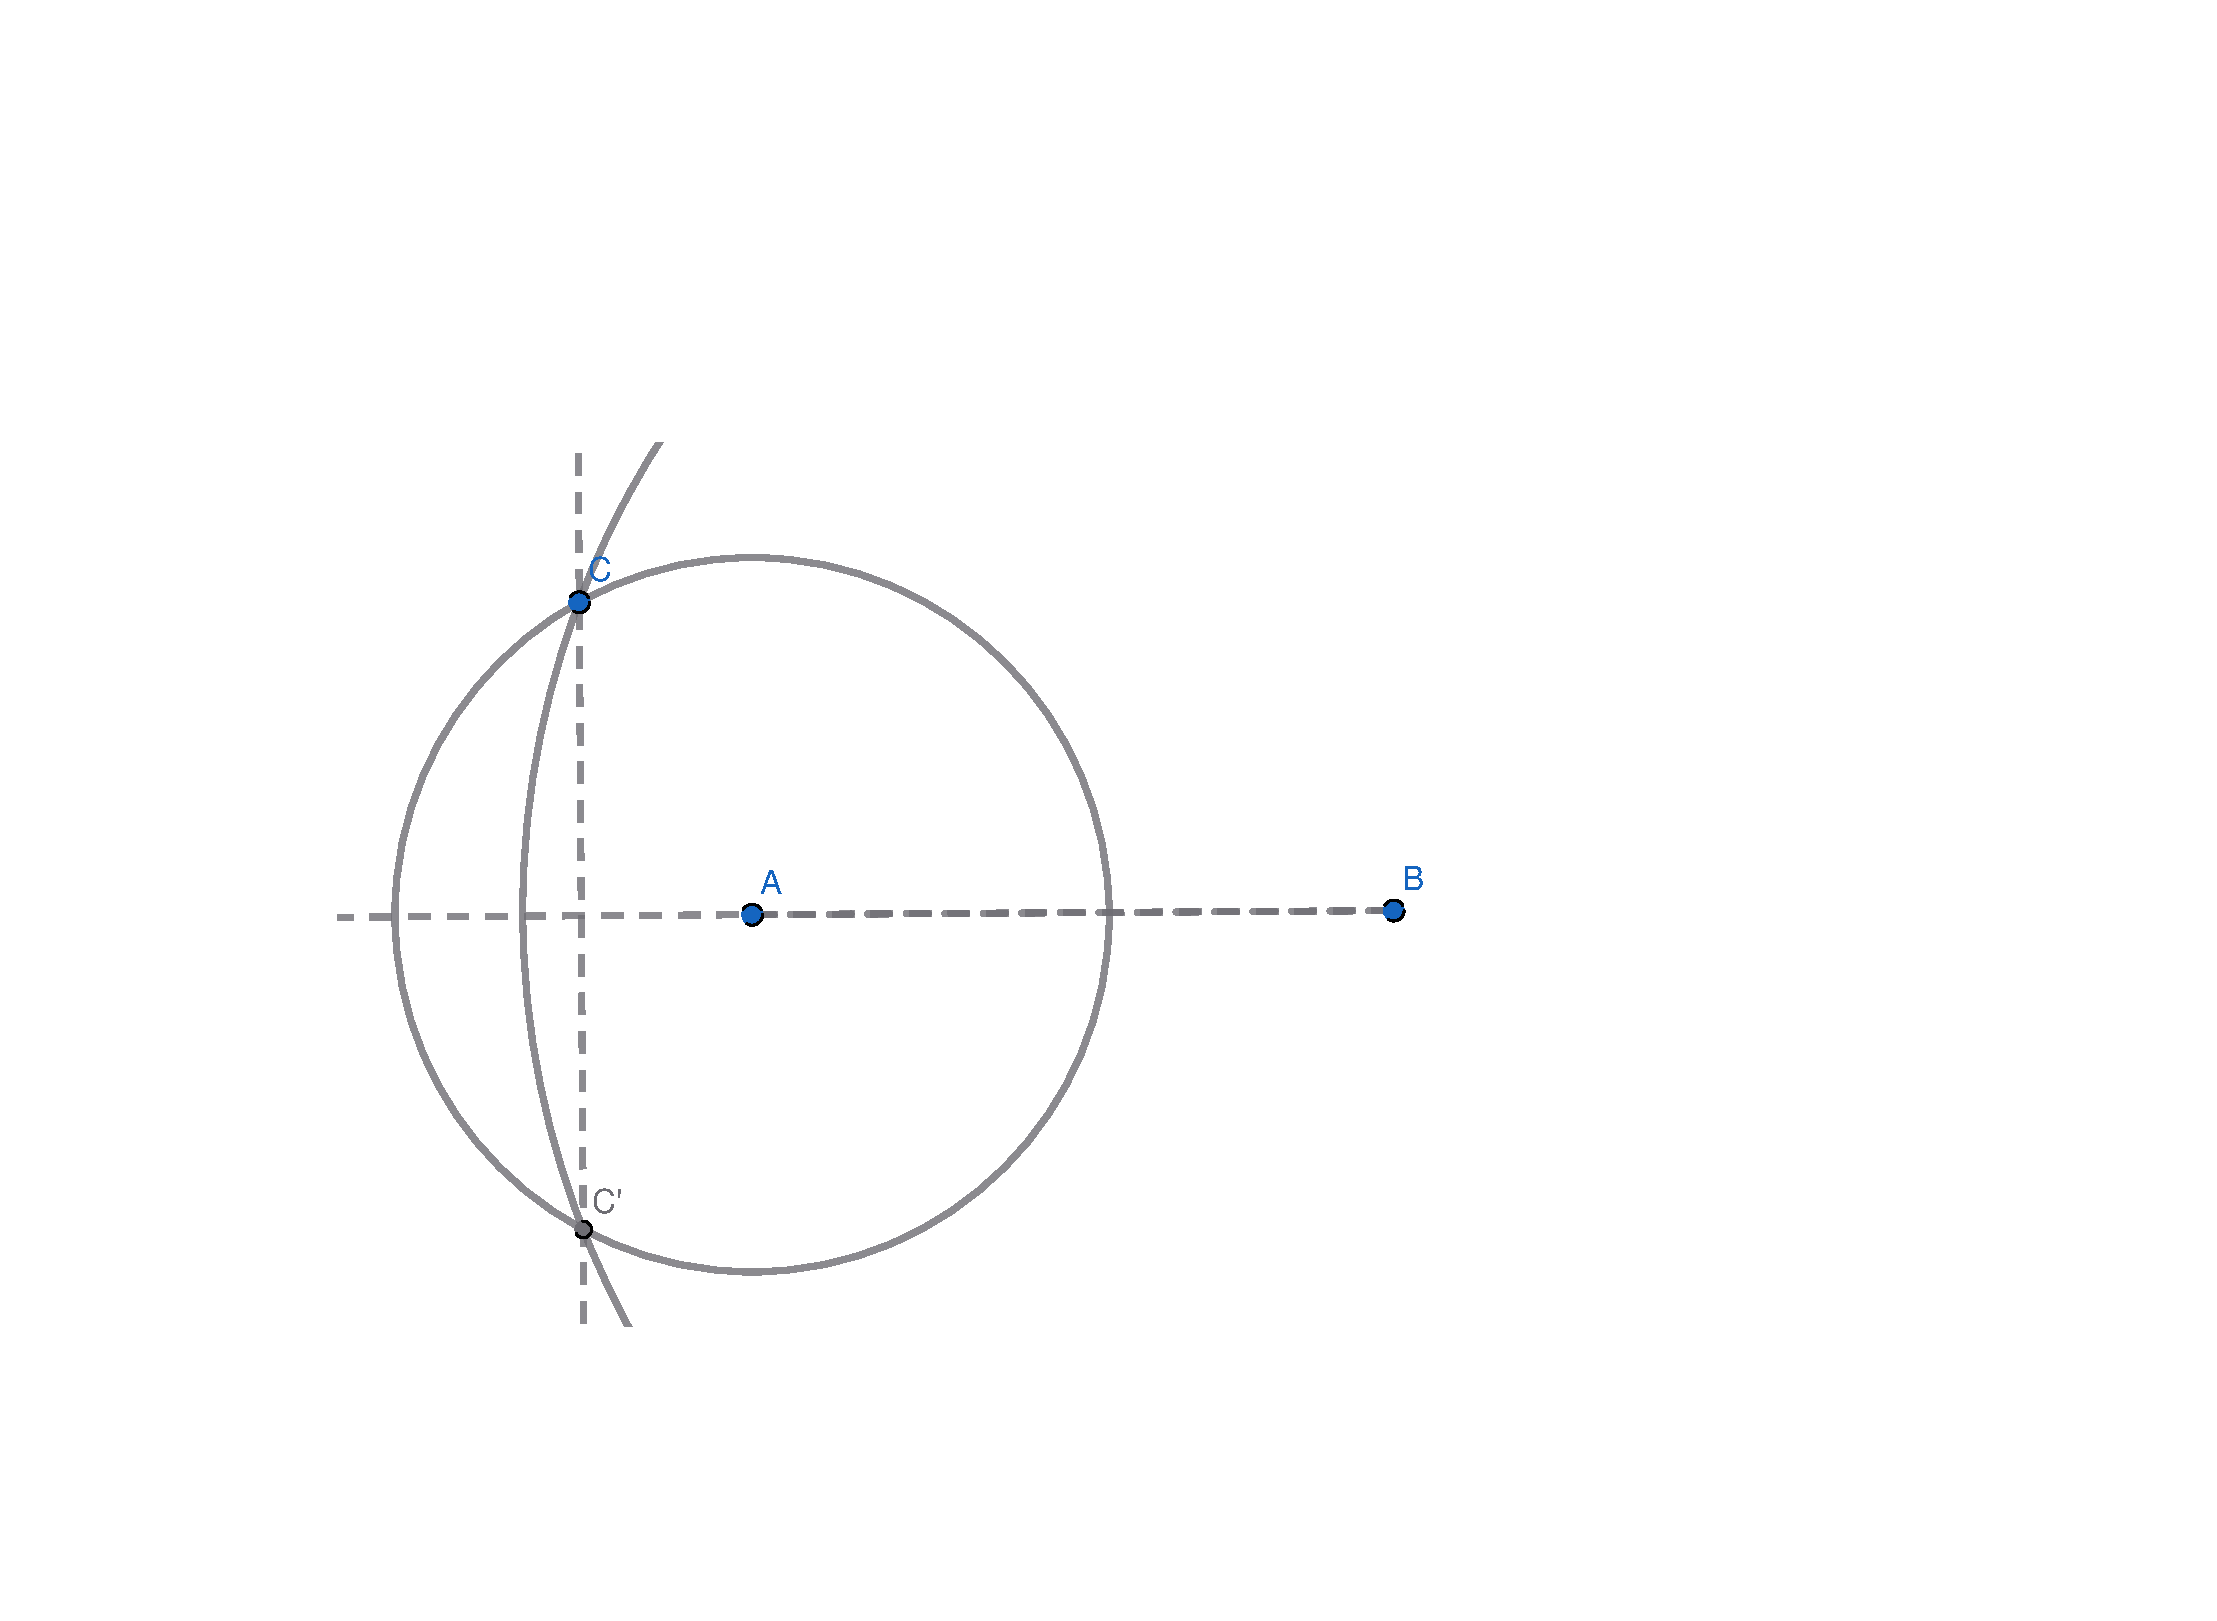
\includegraphics[scale=0.3]{img/perp2}
 \captionof{figure}{Perpendicular line through a point out of the given line.}
 \label{fig:perp-of-point2}
\end{center}
}

\Question{Given a line $l$ and a point $p$ out of it, draw a line parallel to $l$ through $p$.

\vspace{2mm}
From the previous exercise, firstly, draw a perpendicular line $m$ to $l$ through point $p$, then draw another perpendicular line $n$ to $m$ through $p$. It follows that line $l$ is parallel to $n$.
}

\Question{The two legs of a compass close naturally due to gravity when lifted off the plane in ancient Greek times, which couldn't be used to mark off a segment directly as it does today. Given a line segment $AB$, how to mark its length off a line $l$ with such a compass?

\begin{center}
 \includegraphics[scale=0.3]{img/mark-off}
 \captionof{figure}{Mark off segment}
 \label{fig:mark-off}
\end{center}

As shown in \cref{fig:mark-off}, first draw a parallel line to $l$ through $A$ (by the previous exercise); then draw a circle at the center of $A$ with radius of $AB$, which intersects this parallel line at $B'$; connect $A$ and any point $C$ on $l$; finally, draw a parallel line to $AC$ through point $B'$, which intersects $l$ at point $D$. It follows that $AB = CD$.
}

\Question{For $a, b$ being commensurable, show that Euclidean algorithm terminates.

\begin{proof}
As $a, b$ are commensurable, let $a = nc, b = mc$. By the division algorithm $a = bq + r_0$, the remainder $r_0 = a - bq = (n - mq)c$, which is measured by $c$. In the same way, $c$ measures every one of $b > r_0 > r_1 > \dotsb \geq 0$. Divide each by $c$, it turns out to be a series of descending \emph{integers}: $m > n - mq > \dotsb \geq 0$. Since $m$ is finite positive integer, this series is finite, but can not infinitely close to 0.
\end{proof}
}

\Question{For linear Diophantine equation $ax + by = c$, suppose $x_1$, $y_1$ and $x_2$, $y_2$ are two pairs of integral solution. Show that the minimum of $|x_1 - x_2|$ is $b/(a, b)$ and the minimum of $|y_1 - y_2|$ is $a/(a, b)$.

\vspace{2mm}
Denote the greatest common divisor of $a, b$ by $d = (a, b)$. Suppose $x_0, y_0$ for a pair of solution to $ax + by = c$, then below is another pair of solution:

\[
\begin{dcases}
  x = x_0 - k \dfrac{b}{d} \\
  y = y_0 + k \dfrac{a}{d}
\end{dcases}
\]

Because,

\begin{align*}
ax + by &= a (x_0 - k \dfrac{b}{d}) + b (y_0 + k \dfrac{a}{d}) \\
        &= a x_0 - \cancel{ak\dfrac{b}{d}} + b y_0  + \cancel{bk\dfrac{a}{d}} = c
\end{align*}

We shall show that any solution is in this form. Let $x, y$ be some solution. Since $ax + by = c$ and $a x_0 + b y_0 = c$,

\begin{align*}
a (x - x_0) + b (y - y_0)  &= 0 && \text{subtract two equations} \\
\dfrac{a}{d} (x - x_0) + \dfrac{b}{d} (y - y_0) &= 0 && \text{divide both sides by gcd $d$} \\
\dfrac{a}{d} (x - x_0) &= -\dfrac{b}{d} (y - y_0)  && \text{move to the right}
\end{align*}

$\dfrac{a}{d}$ divides the left, hence it also divides the right. But $(\dfrac{a}{d}, \dfrac{b}{d}) = 1$, they are coprime, therefore, $\dfrac{a}{d}$ divides $(y - y_0)$, let

\begin{align*}
y - y_0 &= k \dfrac{a}{d},  &&\text{for some integer }k \\
y &= y_0 + k \dfrac{a}{d} \\
x &= x_0 - k \dfrac{b}{d} && \text{substitute back}
\end{align*}

Which proves that all solutions are in this form. For any two pairs of solution, their different is minimized when $k = 1$. Therefor, the minimum of $|x_1 - x_2|$ is $b/(a, b)$ and the minimum of $|y_1 - y_2|$ is $a/(a, b)$.
}

\Question{List the fewest steps to obtain 6 litres of water with two jugs of 9 and 4 litres.

\vspace{2mm}
\[(0,0) \to (9,0) \to (5,4) \to (5,0) \to (1,4) \to (1,0) \to (0,1) \to (9,1) \to (6,4) \]
}

\Question{Show that the side and diagonal of a regular pentagon are incommensurable.

\begin{proof}
Assume for contradiction, they are commensurable. Denote the side by $mc$, the diagonal by $nc$ for some positive integers $m, n$. As shown in \cref{fig:pentagon-irrational}, since BEC is isosceles triangle, $EC = BE = nc$; Since ABE and FBE are congruent, $AB = FE = mc$. It follows $FC = EC - FE = (n-m)c$. The diagonal of the smaller pentagon, $CD = mc$ and its side $FC = (n -m)c$ is also commensurable. Repeat this, one gets smaller and smaller pentagons infinitely. But this conflicts with the assumption that $m, n$ are finite positive integers. Therefor, the side and diagonal of a regular pentagon are incommensurable.
\end{proof}

\begin{center}
  \includegraphics[scale=0.3]{img/pentagon-irr}
  \captionof{figure}{Side and diagonal of a pentagon.}
  \label{fig:pentagon-irrational}
\end{center}
}

\Question{What the continued fraction of the golden ratio $\phi = \frac{1 + \sqrt{5}}{2}$?

\vspace{2mm}

From $\phi \approx 1.618$, the integral part of $\phi$ is $n_1 = 1$, the remaining part is $\frac{1 + \sqrt{5}}{2} - 1 = \frac{\sqrt{5} - 1}{2}$, we have,
\begin{align*}
  \phi &= 1 + \dfrac{\sqrt{5} - 1}{2} = 1 + \dfrac{1}{\dfrac{1}{\dfrac{\sqrt{5} - 1}{2}}}  \\
  &= 1 + \dfrac{1}{\dfrac{\sqrt{5} + 1}{2}} && \dfrac{\sqrt{5} \pm 1}{2} \text{ are reciprocal of each other} \\
  &= 1 + \dfrac{1}{\phi} = 1 + \dfrac{1}{1 + \dfrac{1}{\phi}} \\
  &= 1 + \dfrac{1}{1 + \dfrac{1}{1 + \dfrac{1}{\dotso}}}
\end{align*}
The continued fraction of the golden ration is $\phi = [1; 1, 1, \dotso]$, a perfect repeating cycle.
}

\end{Answer}

\ifx\wholebook\relax
\chapter{Real}
\else
\section{Real}
\fi

\epigraph{May I have a large container of coffee?}{A short mnemonic for $\pi$}

The Greeks discovered irrational numbers by ruler and compass, which couldn't be the result of arithmetic operation ($+, -, \times, \div$). It arises question what special operation that ruler and compass represent? and the converse question whether all the arithmetic operations can be implemented by ruler and compass? Can we find more irrational numbers through the study of geometric construction?

\section{geometric construction and arithmetic}
\label{sec:geometric-arthimetic} \index{geometric construction}
In Euclidean algorithm, one needs cut off segment $b$ from $a$, which corresponds to subtraction of $a - b$. The reverse construction of extending segment $a$ by length of $b$ (marked off) corresponds to addition of $a + b$ (see \cref{qn:mark-off-segment}). How to realize multiplication of $ab$? one may draw a rectangle with length of $a$ and width of $b$, of which the area is $ab$. However, what the Greeks considering was to draw a ling segment with the length of $ab$, and they figured this out from the tool of similar triangles.

\begin{figure}[htbp]
 \centering
 \includegraphics[scale=0.33]{img/product}
 \caption{Implement multiplication by geometric construction.}
 \label{fig:product}
\end{figure}

\begin{proposition}
Given a unit line segment (of length 1), and two segments of length $a$ and $b$, it possible to construct a line segment of length $ab$.
\end{proposition}

\begin{proof}
As shown in 如\cref{fig:product}, draw a perpendicular line to the unit segment AD (of length 1) at one end and mark off AC of length $b$ (see \cref{qn:perp-of-point}); then extend the unit segment and mark off BD of length $a$. Connect CD to construct a triangle ACD. Draw the parallel line to CD through point B (see \cref{qn:parallel-through-p}), which intersects the extension of AC at point E; it form a bigger triangle of AEB. It follows that the smaller triangle ACD is similar to the bigger triangle AEB (can you justify it?), therefor,

\begin{align*}
\dfrac{1}{b} & = \dfrac{AD}{AC} = \dfrac{AB}{AE} = \dfrac{1 + a}{b + x} && \text{by similar triangles} \\
b + x & = b(1 + a) && \text{cross multiplication} \\
x & = b(1 + a) - b = ab && \text{the length of CE is }ab \qedhere
\end{align*}
\end{proof}

It gives geometric interpretation of multiplication. We shall next establish the correspondence between geometric construction and division. The first step is to realize the reciprocal of $a \ne 0$, which is $\dfrac{1}{a}$, then turn the division into multiplication of $\dfrac{b}{a} = b \times \dfrac{1}{a}$. Using similar triangles again,

\begin{proposition}
Given a unit line segment (of length 1) and a segment of length $a$, it is possible to construct a line segment of length $\dfrac{1}{a}$.
\end{proposition}

\begin{figure}[htbp]
 \centering
 \includegraphics[scale=0.33]{img/reciprocal}
 \caption{Geometric interpretation of reciprocal}
 \label{fig:reciprocal}
\end{figure}

\begin{proof}
As shown in \cref{fig:reciprocal}, draw a perpendicular line to the unit line segment AD (of length 1) at one end and mark off AC of length $a$; extend AC and mark off CE of length 1. Connect CD to form a triangle ACD. Draw a parallel line to CD through point E, which intersects the extension of AD at point B. Connect BD to from a bigger triangle AEB. Sine the smaller triangle ACD is similar to the bigger triangle AEB (can you justify it?),

\begin{align*}
\frac{1}{a} &= \frac{AD}{AC} = \frac{AB}{AE} = \frac{1 + x}{1 + a}  && \text{by similar triangles} \\
a(1 + x) & = 1 + a && \text{cross multiplication} \\
x &= \frac{1 + a}{a} - 1 = \frac{1}{a} && \text{the length of BD is }\frac{1}{a} \qedhere
\end{align*}
\end{proof}

This realizes the reciprocal operation, based on which one can further realizes division. It shows that all the arithmetic operations of $+, -, \times, \div$ have their corresponding geometric realization. Given two segments of length $a$ and $b$, by Pythagorean theorem, it's possible to construct a line segment of length $\sqrt{a^2 + b^2}$. We are going to show how to construct a line segment of length $\sqrt{a}$ directly.

\begin{proposition}\label{thm:sqrt-a}
Given a unit line segment and a line segment of length $a$, it is possible to construct a line of length $\sqrt{a}$.
\end{proposition}

\begin{figure}[htbp]
 \centering
 \includegraphics[scale=0.35]{img/sqrt}
 \caption{Geometric interpretation of square root}
 \label{fig:sqrt}
\end{figure}

\begin{proof}
As shown in \cref{fig:sqrt}, extend the unit line segment (of length 1) and mark off a segment CB of length $a$. Draw a circle with AB as the diameter (draw the perpendicular bisector of AB; then draw the circle at the center of the foot with the bisected length as the radius). Draw a perpendicular line to AB at C, which intersects the circle at point D. Connect AD and BD to form a smaller right triangle ACD and a bigger triangle DCB; they are similar triangles (please justify it).

\begin{align*}
\frac{1}{x} &= \frac{AC}{CD} = \frac{CD}{CB} = \frac{x}{a} && \text{by the similar triangles} \\
x^2 &= a && \text{cross multiplication} \\
x &= \sqrt{a} && \text{the length of CD is }\sqrt{a} \qedhere
\end{align*}
\end{proof}

Thus the operation of extracting square root as well as the arithmetic operations all can be realized by ruler and compass. It turns out that any number, as the result of these operations, can be constructed by ruler and compass. Contrary to what the Pythagoreans thought, geometry was not established based on arithmetic, but arithmetic could be based on geometry. The Greeks were fascinated by exploring varies of problems with ruler and compass.

\subsection{Regular polygons}
\index{regular polygon}
The Greeks constructed many regular polygons with ruler and compass. The side in most cases is irrational. The simplest regular polygon is the equilateral triangle. As shown in \cref{fig:polygon}, given a line segment AB, draw two arcs with the radius of AB at the center of A and B respectively; denote their intersection by C; connecting ABC gives a equilateral triangle. The regular quadrilateral is a square, which can be constructed by connecting the four ends of two perpendicular diameters of a circle. If the radius of the circle is 1, by Pythagorean theorem, the side length is $\sqrt{2}$. From a regular $n$-gon, one can construct a regular $2n$-gon in this way: draw perpendicular bisector of each side, they intersect at a point, which is the circumcenter. Each perpendicular bisector intersects the circumcircle at a point; for each of this point, connect it and the two vertexes next to it of the original $n$-gon, which gives a regular $2n$-gon. For example, the hexagon in \cref{fig:polygon} is obtained from a equilateral.

\begin{figure}[htbp]
 \centering
 \includegraphics[scale=0.35]{img/polygon}
 \caption{Equilateral triangle, square, and regular hexagon.}
 \label{fig:polygon}
\end{figure}

\index{geometric construction!regular pentagon}
Connect each vertex and its circumcircle, which divides the regular hexagon into 6 small equilateral triangles. It follows that if the radius of the circumcircle is 1 then the side of the regular hexagon is 1. For the inscribed equilateral triangle, each side together with two radii of length 1 form a isosceles triangle, whose two sides span $120\degree$. Based on this, it's easy to calculate the side of the inscribed equilateral triangle is $\sqrt{3}$. One may `double' a square to obtain a regular octagon; we leave it as exercise to calculate the side length of the regular octagon. It's a bit hard to construct a regular pentagon, nevertheless, the Greeks worked it out. We show two solutions here and another solution in chapter 6.

\Ref{sec:pentagon-edge} shows when the diagonal of a regular pentagon is 1, the side length is the golden ratio $\phi = \dfrac{\sqrt{5}-1}{2}$. The problem turns out how to construct a line segment of length $\phi$? We know, by Pythagorean theorem, $5 = 2^2 + 1^2$. Given a unit line segment, double it to form a right triangle, the length of its hypotenuse, by Pythagorean theorem, is $\sqrt{2^2 + 1^2} = \sqrt{5}$. Halve the right triangle gives $\dfrac{\sqrt{5}}{2}$; cut the shorter side (of length $\dfrac{1}{2}$) off the hypotenuse, one gets a segment of length$\dfrac{\sqrt{5}-1}{2}$.

\begin{figure}[htbp]
 \centering
 \includegraphics[scale=0.3]{img/phi}
 \caption{construct a line segment of length $\phi = \dfrac{\sqrt{5} - 1}{2}$.}
 \label{fig:phi}
\end{figure}

As shown in \cref{fig:phi}, draw a unit circle and two perpendicular diameters. Next draw the perpendicular bisector of the radius AB, thus the length of the hypotenuse of right triangle ACD is $\dfrac{\sqrt{5}}{2}$. Draw an arc at the center of D with radius of DC, which intersects line BA at point E, then the length of AE is $\dfrac{\sqrt{5} - 1}{2}$.

\begin{figure}[htbp]
 \centering
 \includegraphics[scale=0.35]{img/pentagon-phi}
 \caption{From AE and a radius of length 1, construct three isosceles triangles, which in turn form a regular pentagon.}
 \label{fig:pentagon-phi}
\end{figure}

Next, from a radius of length 1 and the segment of length $\phi$, one may construct a isosceles triangle, namely AHG as shown in \cref{fig:pentagon-phi}(side length of 1, $\phi$, and $\phi$; first draw the base segment, then draw two arcs at the center of each end with radius of $\phi$; finally, connect their intersection and the two ends), and isosceles triangle AGF (side length of 1, 1, and $\phi$), and isosceles triangle AIF (side length of 1, $\phi$, and $\phi$); these three triangles form a regular pentagon.

The second construction comes from Euclid's \emph{The Elements}. When connect the center of a regular pentagon (the center of its circumcircle) and its five vertexes, it divides $360\degree$ into five angles each of $360 \div 5 = 72\degree$. To obtain such an angle, Euclid's idea was to construct a special isosceles triangle, as shown in \cref{fig:isosceles72}, whose base angle is two times of the angle between two sides. Since the sum of angles of a triangle is $180\degree$, it means $\alpha + 2(2\alpha) = 180\degree$, hence the angle between two sides is $\dfrac{1}{5}$ of $180\degree$, which is $36\degree$, and the base angle is $72\degree$.

\begin{figure}[htbp]
 \centering
 \includegraphics[scale=0.35]{img/isosceles72}
 \caption{The isosceles triangle whose base angle is two times of the angle between two sides.}
 \label{fig:isosceles72}
\end{figure}

If we bisect each base angle, then there are in total five angles of $36\degree$. Our goal is to divide $360\degree$, but not $180\degree$, into five equal angles to form a regular pentagon. Because a central angle is twice the inscribed angle subtended by the same arc, each central angle in \cref{fig:triangle-pentagon} is $72\degree$. The corresponding five arcs are of equal length, so do the corresponding chords, which form a regular pentagon.

\begin{figure}[htbp]
 \centering
 \includegraphics[scale=0.35]{img/triangle-pentagon}
 \caption{Bisect each base angle, gives total five inscribed angles of $72\degree$.}
 \label{fig:triangle-pentagon}
\end{figure}

\begin{proposition}[Proposition 11, Book IV, The Elements]
To inscribe an equilateral and equiangular pentagon in a given circle.
\end{proposition}

\begin{proof}
From the above explanation, it's sufficient to show it's possible to construct a isosceles triangle in which the angle between two sides is $36\degree$. As shown in \cref{fig:triangle-pentagon}, the ratio of base and side of the isosceles triangle ($BC:AB$) equals the ratio of side and diagonal of the regular pentagon. \Cref{sec:pentagon-edge} shows this ratio is the golden ratio of $\phi = \dfrac{\sqrt{5} - 1}{2}$. The remaining steps are same as in the first construction: (1) draw a right triangle with sides of $\dfrac{1}{2}$ and 1, by Pythagorean theorem, the length of the hypotenuse is $\dfrac{\sqrt{5}}{2}$; then cut $\dfrac{1}{2}$ off the hypotenuse, which gives the golden ratio $\phi$. (2) draw a isosceles triangle ABC with sides of $1$, $\phi$, and $1$, in which the angle between two sides is $36\degree$; draw its circumcircle. (3) bisect each base angle, intersects the circumcircle at point D and E respectively; connect A, B, C, D, E to form a regular pentagon.
\end{proof}

\index{Gauss} \label{sec:Gauss-17-gon}
We'll give the third construction of regular pentagon in Chapter 6 based on complex number and Euler's formula. The Greeks met great difficulty in constructing regular heptagon with ruler and compass. About 2,000 years later in 1792, a young man was about to choose between theology and mathematician. He was born in Brunswick as the only child of a poor family. His father earned living mainly from manual labor. At the age of seven, he started elementary school. His teacher once asked the students to calculate the sum of $1 + 2 + \dotsb + 100$; he observed that $1 + 100 = 2 + 99 = \dotso = 50 + 51 = 101$, in total 50 such pairs, so the answer was 5050. This amazed his teachers. Later, duke of Brunswick heard about him and granted him financial assistance to continue his education. At the age of 15 when thinking about if next to study theology or mathematics, the young man proved a regular polygon of 17 sides can be constructed by ruler and compass alone\cite{Gauss-Britannia-2025}. Being so exciting and motivated, that he decided to devoted to mathematics. This young man was Carl Friedrich Gauss.

\begin{figure}[htbp]
 \centering
 \includegraphics[scale=0.5]{img/gauss-17gon}
 \caption{A stamp to memorize Gauss solved geometric construction of a regular polygon of 17 sides.}
 \label{fig:gauss-17gon}
\end{figure}

\label{sec:geometric-cons-polygon}
We skipped the detailed steps to construct a regular polygon of 17 sides. Richelot and Schwendenwein constructed the regular 257-gon in 1832. J. Hermes constructed the regular 65537-gon in 1894; he spent ten years on it and deposited the manuscript in a large box in the University of Göttingen. We stop for a while: don't these numbers look familiar? The equilateral triangle can be constructed, $3 = 2^{2^0} + 1$; the regular pentagon can be constructed, $5 = 2^{2^1} + 1$; the regular 17-gon can be constructed, $17 = 2^{2^2} + 1$; the regular 257-gon can be constructed, $257 = 2^{2^3} + 1$; and the regular 65537-gon can be constructed, $65537 = 2^{2^4} + 1$. They are Fermat's numbers! Once construct a regular $n$-gon, by perpendicular bisecting each side, one can construct a regular $2n$-gon. It turns out that a regular polygon of $2^k m$ sides can be constructed if a regular $m$-gon can be constructed, where $m$ is odd. What Gauss discovered was when $m$ was a product of distinct Fermat's prime numbers, the regular $m$-gon can be constructed by ruler and compass only. It was proven by French mathematician Wantzel\footnote{Pierre Wantzel was at the age of 23 this year. He died at the age of 34 due to irregular work and life. He usually worked during the evening, not going to bed until late in the night, then reading, and got but a few hours of agitated sleep, alternatively abusing coffee and opium, taking his meals, until his marriage, at odd and irregular hours.} in 1837, and was named Gauss-Wantzel theorem.

\index{Gauss-Wantzel theorem}
\begin{theorem}[Gauss-Wantzel]
The regular polygon of $p$ sides, where $p$ is prime, can be constructed by ruler and compass if and only if $p=2^{2^n} + 1$, in other words, $p$ is Fermat's number. The regular polygon of $n$ sides can be constructed by ruler and compass if and only if $n=2^k p_1 p_2 \dotsm p_m$ where $p_i$ are distinct Fermat's prime numbers \cite{Edward-1977}.
\end{theorem}

\subsection{Limitations of geometric construction}
Gauss-Wantzel theorem shows there are limitations of geometric construction: there exist things that can't be constructed by ruler and compass only. For example, one can not construct a regular heptagon, nor he can obtain a line segment equal the side length of a regular heptagon\footnote{Here we limit to use the ruler without marks, i.e., a straightedge, and compass only, otherwise, it's possible.}. Since ruler and compass can implement arithmetic operations and square root, the side length of a regular heptagon can't be calculated from a series of arithmetic operation and taking square root of rational numbers. It is a irrational number, but we don't know how to represent it arithmetically. Using trigonometrical functions, if the radius of the circumcircle of a regular heptagon is 1, then its side length is $x = 2\sin(\dfrac{180\degree}{7})$ as shown in \cref{fig:heptagon}.

\begin{figure}[htbp]
 \centering
 \includegraphics[scale=0.35]{img/heptagon}
 \caption{Represent the side length of a regular heptagon. Suppose the length of the radius of the circumcircle is 1, the regular heptagon divides $360\degree$ into seven equal angles, each $\theta = \dfrac{360\degree}{7}$, the $\sin$ of its half is $\sin(\dfrac{180\degree}{7})$, which is half of the side length.}
 \label{fig:heptagon}
\end{figure}

\index{three geometric construction problems}
The Greeks didn't know about this, nevertheless, they strictly followed the tradition from Plato, solved one problem after another with ruler and compass only. However, there were three popular problems about geometric construction they couldn't solve:

\begin{enumerate}[(1)]
\item Duplication of the cube. To double the volume of a cube. According to a legend, a plague broken out in Athens; people went to the Tempo of Apollo to pray for help. The priest declared that Apollo demanded the cubic altar be doubled in volume to dispel the disaster. Nobody could solve it (with ruler and compass only). If denote the side of the original cube by 1, the problem is asking to construct a line segment of length $\sqrt[3]{2}$.

\item Trisection of an angle. Given an arbitrary angle $\theta$, construct an angle of $\dfrac{\theta}{3}$. Note there exists some special angle that can be trisected, for example, $90\degree$, $135\degree$, $180\degree$, and $360\degree$, but an arbitrary angle $\theta$ can not necessarily be trisected, for example $60\degree$.

\item Squaring the circle. Construct a square whose area equal to the area of a given circle. If the radius of the circle is 1, the problem is to construct a square with side length of $\sqrt{\pi}$.
\end{enumerate}

It was not until the 19 century, as the development of abstract algebra, particularly field theory, group theory, and Galois theory, that people finally solved all three problems -- they are all insoluble; it's impossible to duplicate the cube, trisect of an arbitrary angle, or square the circle with ruler and compass only\footnote{Wantzel proved that neither duplication of the cube nor trisection of an angle was geometric constructible; Lindemann proved $\pi$ was a transcendental number in 1882, hence the problem of squaring the circle was non-constructible.}.

\index{analytic geometry}
Despite it need abstract algebra and field theory to prove Gauss-Wantzel theorem, we may give some simplified explanation to it (see the prove outline in \cref{app:gauss-wantzel-theorem}). In the 17th century, Descartes developed analytic geometry (also known as coordinate geometry, Fermat independently developed analytic geometry with Descartes), reestablished geometry on top of algebra (equation and function). It gave the new interpretation on the ancient Greek ruler and compass construction.

\subsubsection{The straight line through two points}
A straight line in a plan can be described by function $y = kx + b$, where $k$ is the slope, and $b$ is the interception. Vertical lines are specially represented as $x = a$. The postulate 1 in Euclid's \emph{The Elements} \enquote{, To draw a straight line from any point to any point.} is interpreted in analytic geometry as the straight line that passes through two points of $(x_1, y_1)$ and $(x_2, y_2)$, where $x_1 \ne x_2$. The two points satisfy the same linear equation:

\[
\begin{cases}
y_1 = k x_1 + b \\
y_2 = k x_2 + b
\end{cases}
\]

Solving this system of two unknowns, namely $k$ and $b$: subtract the two equations to obtain $k = \dfrac{y_2 - y_1}{x_2 - x_1}$, then substitute back to obtain $b = y_1 - k x_1$. Alternatively, one may apply the \enquote{two points form} as shown in \cref{fig:line2p},

\[
\frac{y - y_1}{x - x_1} = \frac{y_2 - y_1}{x_2 - x_1}
\]

\begin{figure}[htbp]
 \centering
 \includegraphics[scale=0.35]{img/line2p}
 \caption{Two points form: Draw the straight line that passes two points $A$ and $B$. Suppose $P = (x, y)$ is some point on the line, the right triangles ACB and AQP are similar, hence $\dfrac{PQ}{QA} = \dfrac{BC}{CA}$.}
 \label{fig:line2p}
\end{figure}

When $x_1 = x_2$, then the line that passes the two points is vertical, the equation is $x = x_1$. Denote the distance between the two points by $r$, by Pythagorean theorem, $(x_2 - x_1)^2 + (y_2 - y_1)^2 = r^2$, then $r = \sqrt{(x_2 - x_1)^2 + (y_2 - y_1)^2}$. In other words, $r$ is a square root; it is the positive solution of a quadratic equation defined by the Pythagorean theorem (with $r$ as the unknown). Essentially, the meaning of \enquote{to draw a straight line from any point to any point} in analytic geometry is this: suppose the coordinates of the two points are in set $K$ (for example, $K = \mathbb{Q}$ means the coordinates are rational points. $K$ may be \enquote{bigger} set containing rationals), then the straight line is a linear function with coefficients in $K$. The distance between the two points is a solution of a quadratic equation with coefficients in $K$.

Given a straight line and a point, one may draw the perpendicular line through this point. In analytical geometry, the perpendicular line to a line defined by $y = kx + b$ has the form of $y = -\dfrac{1}{k} x + b'$, where $k \ne 0$. If it passes point $(x_0, y_0)$, then $y_0 = -\dfrac{1}{k} x_0 + b'$, whence, $b' = y_0 + \dfrac{1}{k}$. For the special case of vertical line $x = a$, the perpendicular line (horizontal) has the form of $y = b$. If it passes point $(x_0, y_0)$, then the equation is determined by $y = y_0$. Basically, if the slope of the given line and the coordinate that the perpendicular line passed through are in set $K$ containing rationals, then the perpendicular line is some linear equation with coefficients in $K$.

\subsubsection{A circle with a center and radius}

The Postulate 3 in \emph{The Elements} states: to describe a circle with any center and radius. Given three points $O, M, N$ in a plane, one may draw a circle at the center of $O$ with the radius equal the length of segment $MN$. The radius $r = \sqrt{(x_m - x_n)^2 + (y_m - y_n)^2}$, is determined by the coordinates of $M, N$, and Pythagorean theorem. From the school math, the circle at the center of $(a, b)$ with radius of $r$ can be described by equation $(x - a)^2 + (y - b)^2 = r^2$. Basically, if the coordinates of the three points are in set $K$ containing rationals, then the circle is described by a quadratic equation with coefficients in $K$.

\subsubsection{intersection}
There are three types of intersection: a line intersects another line, a line intersects a circle, and a circle intersects another circle. The intersection of two lines is the solution to two linear equations,

\[
\begin{cases}
y = k_1 x + b_1 \\
y = k_2 x + b_2
\end{cases}
\]

If the two lines are not parallel ($k_1 \ne k_2$), then the solution is uniquely determined. If $k_1 = k_2$ but $b_1 \ne b_2$, then the two lines are parallel, hence no solution, no intersection. If $k_1 = k_2$ and $b_1 = b_2$, then the two lines overlap, they have infinitely many \enquote{intersections}. Basically, for nonparallel lines intersect; if the coefficients of the linear equations are in set $K$ containing rationals, then the coordinates of the intersection are in $K$.

The relation between a line and a circle is described by a system of,

\[
\begin{cases}
(x - a)^2 + (y - b)^2 = r^2 \\
y = kx + c
\end{cases}
\]

Substitute the second equation to the first,

\begin{align*}
& (x - a)^2 + (kx + c - b)^2 = r^2  &&\text{substitute }y = kx + c \\
& x^2 + a^2 - 2ax + k^2x^2 + d^2 + 2kdx - r^2 =0 && \text{let }d = c - b \\
& (1 + k^2)x^2 + 2(kd - a)x + a^2 + d^2 - r^2 = 0 && \text{collect terms} \\
& Ax^2 + 2Bx + C = 0
\end{align*}

where $A = 1 + k^2, B = kd - a, C = a^2 + d^2 - r^2$, the discriminant of this quadratic equation is $\Delta = \sqrt{4B^2 - 4AC} = 2\sqrt{B^2 - AC}$. There are three cases:
\begin{itemize}
\item if $B^2 < AC$, the line is separate from the circle, hence no intersection.
\item if $B^2 = AC$, the line is tangent to the circle, they have exactly one common point.
\item if $B^2 > AC$, the line intersects the circle, they have two distinct common points.
\end{itemize}

The relation between two circles is described by two equations,

\[
\begin{cases}
(x - a)^2 + (y - b)^2 = r_1^2 \\
(x - c)^2 + (y - d)^2 = r_2^2
\end{cases}
\]

We can convert it to a quadratic equation, then by its discriminant, $\Delta >, =, < 0$, to determine if the two circles are separate (including the case that a circle is inside the other without touching), externally/internally tangent to each other, or intersect each other. Basically, for line and circle, circle and circle, the coordinates of their intersection, if exists, are solutions to some quadratic equation. The coefficients may not be rational, for example, in \cref{fig:P1}, neither the slope $k$ nor intercept $b$ of the linear equation describing line CE is rational.

As such, we describe ruler and compass construction with equations through Descartes's analytical geometry. This is the tool that helps us understand the capability/limitation of geometric construction. Given two points A and B in a plane, we define one as the origin $(0, 0)$, the other as $(1, 0)$, hence also define the unit segment of length 1. We may conduct a round of ruler and compass construction, including: (1) connect all known points to form a set of straight lines, $\mathbf{L}_1$; (2) draw circles at the center of each point, with the radius of each known segment; denote this set of circles by $\mathbf{C}_1$; (3) mark the intersections between lines, lines and circles, and circles; denote the set of these points by $\mathbf{P}_1$.

\begin{figure}[htbp]
 \centering
 \includegraphics[scale=0.35]{img/P1}
 \caption{The set of points from the first round of ruler and compass construction: $\mathbf{P}_1 = \{A, B, C, D, E, F\}$}
 \label{fig:P1}
\end{figure}

As shown in \cref{fig:P1}, after the first round of ruler and compass construction, we obtained a line, two circles, and six points. \emph{All} the constructed length are solutions to some linear or quadratic equations with rational coefficients. Denote the set of these numbers by $K_1$. We next conduct the second round of ruler and compass construction, including: (1) connect all points in $\mathbf{P}_1$ to form a new set of lines $\mathbf{L}_2$; (2) Draw circles with all combinations of three points $O, M, N$ in set $\mathbf{P}_1$, at the center of $O$ with radius of segment $MN$; denote the set of these circles by $\mathbf{C}_2$; (3) Mark the intersections between lines in $\mathbf{L}_2$, between every line in $\mathbf{L}_2$ and every circle in $\mathbf{C}_2$, and between circles in $\mathbf{C}_2$; denote the set of these points by $\mathbf{P}_2$.

The constructed magnitudes from the second round are solutions to linear and quadratic equations with coefficients in $K_1$; denote the set of these magnitudes as $K_2$. We repeat, round after round, which construct more and more magnitudes in $K_1, K_2, K_3, \dotsc$ including numbers like $1 + \sqrt{2} + \sqrt{2\sqrt{3} - \sqrt{5}}$. Can you give some more examples?

The size of the set, as the round of construction increases, grows exponentially. The construction continues infinitely, every round is equivalent to solving linear and quadratic equations with coefficients constructed from previous round. The set of all constructible numbers is infinite, however, it does not contain $\sqrt[3]{2}$ (see \cref{app:gauss-wantzel-theorem}). Because it is not a solution to any linear or quadratic equation with rational coefficients, nor a solution to any linear or quadratic equation with coefficients in $K_1$, nor a solution to any linear or quadratic equation with coefficients in $K_2$ ... It can not be constructed by ruler and compass\footnote{$\sqrt[3]{2}$ is the unique real solution to cubic equation $x^3 - 2 = 0$, the other two roots are complex numbers of $-\sqrt[3]{2}\dfrac{1 \pm \sqrt{3}}{2}$, see chapter 6.}. Thereby, it's impossible to duplicate a cube. As shown in \cref{fig:heptagon}, the side length of a regular polygon of $n$ sides is $x = 2\sin(\dfrac{360\degree}{2n})$. It can be constructed by ruler and compass if and only if it is a solution to some linear or quadratic equation with coefficients in some $K_i$ (i.e., in $K_{i+1}$).

By Gauss-Wantzel theorem, the regular polygon of 18 sides can't be constructed by ruler and compass because $18 = 2 \times 3^2$, isn't product of distinct Fermat's prime numbers and power of 2. It follows that, $\dfrac{1}{18}$ of $360\degree$, namely $20\degree$, can not be constructed, hence it's impossible to trisect $60\degree$. This shows the problem of trisection of an angle is unsolvable.

\begin{figure}[htbp]
 \centering
 \includegraphics[scale=0.4]{img/Descartes}
 \caption{René Descartes (1596 - 1650). Portrait after Frans Hals, Louvre Museum}
 \label{fig:Decartes}
\end{figure}

\index{Descartes}
\begin{mdframed}
René Descartes was a French philosopher, mathematician, and scientist. Descartes also has a Latinized name: Cartesius, as Latin was the widely used academic language in his time. Its adjective form is Cartesian. This is source of the terms like Cartesian coordinate, Cartesian product, and etc.

Descartes was born in La Haye, France in 1596. His father was a member of the Parlement of Brittany at Rennes. His mother died a year after giving birth to him, and so he was not expected to survive. His father then remarried in 1600. Descartes lived with his grandmother at La Haye. His health was poor when he was a child. Throughout his childhood, up to his twenties, he was pale and had a persistent cough.

In 1607, he entered the Jesuit college of La Flèche, where he was introduced to mathematics and physics, including Galileo's work. While in the school his health was poor and, instead of rising in the morning like the other boys, he was granted permission to remain in bed until 11:00 AM, a custom he maintained until the year of his death.

After graduation in 1614, he studied for two years at the University of Poitiers. He received a law degree in 1616 to comply with his father's wishes but he quickly decided that this was not the path he wanted to follow. He returned to Paris, then became a volunteer in the army of Maurice of Nassau. In the army, Descartes started studying mathematics and mechanics under the Dutch scientist Isaac Beeckman, and began to seek a unified science of nature.

%% After this time in Holland he left the service of Maurice of Nassau and travelled through Europe. In 1619 he joined the Bavarian army and was stationed in Ulm. An important event in his life was three dreams he had in November 1619. These he believed were sent by a divine spirit with the intention of revealing to him a new approach to philosophy. The ideas from these dreams would dominate much of his work from that time on.

From 1620 to 1628 Descartes travelled through Europe, spending time in Bohemia, Hungary, Germany, Holland, through Switzerland to Italy, then Venice and Rome. He returned Paris in 1625. His Paris home became a meeting place for philosophers and mathematicians and steadily became more and more busy. By 1628 Descartes, tired of the bustle of Paris, the house full of people, and of the life of travelling he had before, decided to settle down where he could work in solitude. He gave much thought and chose Holland. What he longed for was somewhere peaceful where he could work away from the distractions of a city such as Paris yet still have access to the facilities of a city. He told his friend Marin Mersenne where he was living so that he might keep in touch with the mathematical world, but otherwise he kept his place of residence a secret. Descartes wrote all his major work in Netherlands in about 20 years, initiating a revolution in mathematics and philosophy. In 1633, Galileo was condemned by the Italian Inquisition, and Descartes abandoned plans to publish {\em Treatise on the World}, his work of the previous four years. Nevertheless, in 1637 he published parts of this work in three essays: {\em The Meteors}, {\em Dioptrics} and {\em Geometry}, preceded by an introduction, his famous {\em Discourse on the Method}.

In {\em Geometry}, Descartes exploited the discoveries he made with Pierre de Fermat. This later became known as analytic geometry or Cartesian geometry. Descartes continued to publish works concerning both mathematics and philosophy for the rest of his life. In 1641 he published a metaphysics treatise, {\em Meditations on First Philosophy}. It was followed in 1644 by {\em Principles of Philosophy}. He became the most influential philosophers in Europe.

In 1649 Queen Christina of Sweden persuaded Descartes to go to Stockholm. However, the Queen wanted to draw tangents at 5 AM. Descartes broke his lifetime habit of getting up at 11 o'clock. After only a few months in the cold northern climate, walking to the palace for 5 o'clock every morning, he died of pneumonia February 1650 at the age of 54.

Descartes left the best known philosophical statement \enquote{I think, therefore I am.} (cogito, ergo sum in Latin). He laid the foundation for 17th-century continental rationalism. He was well-versed in mathematics as well as philosophy, and contributed greatly to science as well. He is credited as the father of analytical geometry, the bridge between algebra and geometry—used in the discovery of infinitesimal calculus and analysis. Descartes was also one of the key figures in the Scientific Revolution.
\end{mdframed}

\section{$\pi$}
\index{$\pi$}
$\pi$ is our old friend in school math. We do not know when people discovered that the ratio of circumference and diameter being constant; it might came from experience of measurement. \Cref{fig:ybc7302} shows a Babylonian tablet (about 1900 - 1600 BCE) in the Peabody Museum of National History in Yale University. Its catalog number is YB7302. \Cref{fig:proust-ybc7302} is the figure sketched by French historian Christine Proust\cite{Proust-2016}. We can read the cuneiform numbers (see chapter 1) 3 along the circle, 45 inside the circle, and 9 outside the circle. The Babylonian numerals were 60-based. According to Proust's interpretation, 3 is the circumference, and 9 is the square of the circumference. We know the circumference $C = 2\pi r$, where $r$ is the radius. Its square is $4\pi^2 r^2$, hence the relation between area and circumference is,

\begin{figure}[htbp]
 \centering
 \subcaptionbox{Babylonian tablet collected in Yale University. It was inscribed with a circle and cuneiform numerals, which concerning circumference and area of a circle. \label{fig:ybc7302}}{\includegraphics[scale=0.4]{img/ybc7302}}
 \subcaptionbox{3, 9, and 45 in cuneiform. \label{fig:proust-ybc7302}}{\includegraphics[scale=0.5]{img/proust-ybc7302}}
 \caption{$\pi$ in Babylonian tablet.}
\end{figure}

\[
S = \pi r^2 = \frac{4 \pi^2 r^2}{4\pi} = \frac{C^2}{4\pi}
\]

If taking $\pi \approx 3.14$, then the area $S = 9/4\pi \approx 0.72$, but how to interpret the numeral 45? Though the Babylonian numerals were position based system, it had problem of lacking zero and decimal point. In fact, it should be 0.45 in 60-based system, which equals $\dfrac{45}{60} = 0.75$ in decimal. In turn, we can calculate the value of $pi$ that the Babylonians used:

\[
\pi = \frac{C^2}{4S} = \frac{9}{4 \times 0.75} = 3
\]

People soon unsatisfied with its precision. For example, the problem 50 in Rhind papyrus in ancient Egypt (about 1650 BCE) was about the area of circle: For a round shaped land, its diameter is 9 khet, what is its area? Ahmes, the author, solved it as this: drop $\dfrac{1}{9}$ of the diameter, which is 1, it remains 8. 8 times 8 equals 64, hence the area is 64 setat. We can calculate the value of $\pi$ in ancient Egypt:

\begin{align*}
S & = \pi r^2 = \pi (\frac{d}{2})^2 \\
\pi & = 4\frac{S}{d^2} = 4(\frac{8}{9})^2 \approx 3.16
\end{align*}

\subsection{Cyclotomic method}
\index{cyclotomic method}
Archimedes was the first one who gave the upper and lower bounds of $\pi$. He developed the method that later mathematicians followed for 1,800 years. From the Egyptians result, we estimate,

\begin{proposition}
The value of $\pi$ is between 3 and 4.
\end{proposition}

It's still the best practice in school, that the teacher guided students to use a rope and a ruler to measure the circumference and diameter, it's interesting to rediscover $\pi$. The approximate value $3.14$ becomes everyone's memory in childhood. It's definitely between 3 and 4, why need prove? Proof is the Greek tradition, the sprite of geometry -- be rigorous and perfect. It is in pursuing rigor and perfection, the Greeks developed tools and techniques. For example, Archimedes greatly developed the method of exhaustion when approximating $\pi$, he achieved the best ever result.

\begin{proof}
First, we are going to show $\pi > 3$. As shown in \cref{fig:inscribed-hexagon}, consider the unit circle with radius of 1 and the inscribed regular hexagon. Connect each vertex and the center; it divides the circle into 6 congruent equilateral triangles (each triangle is isosceles because the sides equal the radius; besides, each angle between the sides equal $\dfrac{360\degree}{6} = 60\degree$). Because the length of the radius is 1, the side length of the equilateral triangle is 1, it follows the circumference of the regular hexagon is 6. Since the circumference of the circle is longer than the inscribed hexagon,

\begin{figure}[htbp]
 \centering
 \subcaptionbox{The unit circle and its inscribed regular hexagon. \label{fig:inscribed-hexagon}}{\includegraphics[scale=0.4]{img/hexagon}}
 \subcaptionbox{The unit circle and its circumscribed square. \label{fig:square-hexagon}}{\includegraphics[scale=0.4]{img/square-hexagon}}
 \caption{The unit circle, its inscribed regular hexagon, and its circumscribed square.}
\end{figure}

\[
\pi = \frac{C}{d} = \frac{C}{2} > \frac{6}{2} = 3
\]

Next, we shall show $\pi < 4$. As shown in \cref{fig:square-hexagon}, draw the circumscribed square of the unit circle. It's side length equals the length of diameter, which is 2. The circumference of the square is 8, and it is longer than the circumference of the circle.

\[
\pi = \frac{C}{d} = \frac{C}{2} < \frac{8}{2} = 4
\]

It proves $3 < \pi < 4$.
\end{proof}

This was almost the same idea that Archimedes approximating $\pi$; the only difference was that instead of square Archimedes used the same regular polygon to inscribe and circumscribe the circle as shown in \cref{fig:pi-exhaustion}. Suppose the diameter is 1, the circumference of the circle is $\pi$. It is longer than the inscribed regular polygon but shorter than the circumscribed regular polygon.

\begin{figure}[htbp]
 \centering
 \includegraphics[scale=0.5]{img/pi-exhaustion}
 \caption{Apply method of exhaustion to $\pi$.}
 \label{fig:pi-exhaustion}
\end{figure}

\[
  C_i < \pi < C_o
\]

\index{method of exhaustion}
where $C_i$ and $C_o$ are the inscribed and circumscribed circumferences of the regular polygon. By increasing the number of sides $n$, Archimedes was able to obtain arbitrary precise range that containing $\pi$ as he wanted. This was called the method of exhaustion, from where arose the idea of calculus. Given whatever small precision, for example $\epsilon = 0.00 \dotso 01$, one can find a large enough natural number $n$, such that the inscribed and circumscribed regular polygons more than $n$ sides satisfying both $C_o - \pi$ and $\pi - C_i$ are less than $\epsilon$. Informally speaking, when $n$ increases infinitely large, both $C_o$ and $C_i$ are close to $\pi$. It was said that Antiphon the Sophist (about 480 - 410 BCE) was the first who developed the method of exhaustion. When studying the problem of squaring the circle, Antiphon started from a inscribed square, and went on approximating the circle with regular octagon, 16-gon, and so on. The difference between the circle and regular polygon exhausted step by step. Antiphon argued that the regular polygon would arbitrarily close to the circle. Later, Eudoxus of Cnidus improved this method by making it rigorous. The method of exhaustion became a useful tool to solve geometric problems regarding area and volume. Eudoxus applied it to show the volume of a pyramid is one third of a prim with the same height and base area; the volume of a cone is one third of a cylinder with the same height and area. These result were recorded in Book XII of Euclid's \emph{The Elements}\cite{HanXueTao16}.

古希腊将穷竭法发展到最高成就的当属阿基米德,他使用内外多边形计算出了圆周率范围:$\dfrac{223}{71} < \pi < \dfrac{22}{7}$。取上下两个边界的平均值,阿基米德相当于计算出$\pi \approx 3.1418$,误差仅有0.0002。这在没有位值制10进制计数系统的古希腊是一个极为惊人的成就。今天西方仍然广泛使用$\dfrac{22}{7}$进行日常计算。除此之外,阿基米德还证明了圆面积公式,球体、锥体的表面积和体积公式,甚至找到了计算抛物线下面积的方法。被称为古希腊的数学之神。

\begin{figure}[htbp]
 \centering
 \includegraphics[scale=0.33]{img/FieldsMedal}
 \caption{菲尔兹奖章上的阿基米德像}
 \label{fig:Archimedes-book}
\end{figure}

\index{数学家!阿基米德}
\begin{mdframed}
阿基米德(前287年~前212年),生于西西里岛的叙拉古王国。早年曾经在古希腊的学术中心亚历山大城跟随欧几里得学习。阿基米德后来回到了叙拉古,他的许多学术成果都是通过和亚历山大城的学者之间的往来信件保存下来的。虽然有关阿基米德的生平没有详细的记载,但是关于他的各种故事却广为流传、脍炙人口。最著名的故事就是国王的王冠。叙拉古国王不知道他的王冠是否是纯金的,大臣们也一筹莫展,于是去请教阿基米德。阿基米德一直解不开这个难题,他废寝忘食,直到有一天洗澡的时候,看着浴缸里的水溢出来,突然得到了灵感。他从浴缸里一跃而出,光着身子跑到大街上,边跑边喊“尤里卡!尤里卡!”,这句希腊语Eureka的意思是“我找到了!”。阿基米德利用浮力和比重,最终发现王冠掺了假。他的这一发现就是每一个中学生都要学习的“阿基米德定律”。尤里卡后来被人们用来形容找到灵感的那一刹那。

阿基米德发现球的体积是其外接圆柱体积的2/3。他觉得这一关系无比的美妙,因此决定死后在墓碑上刻一个内接圆柱的球体。公元前214年,第二次布诺战争爆发了。面对敌人的围城,传说阿基米德设计了巨大的抛物面镜,把阳光汇聚到帆上烧毁了敌人的战船。阿基米德还设计了巨大的机械武器,可以瞬间击毁罗马战船。后来罗马军队攻陷了叙拉古城,一个罗马士兵冲进阿基米德家里。阿基米德正专注地在沙地上画着几何图形进行思考,他说出了那句著名的话:“不要打扰我的圆。”感到被冒犯的罗马士兵挥刀杀死了面前的这个老人。古希腊最伟大的数学家就此停止了思考。
\end{mdframed}

阿基米德之后,古希腊天文学家和数学家托勒密从古巴比伦的60进制中汲取了营养。他通过正360边形来逼近$\pi$,得到结果:

\[
\pi \approx 3 + \frac{8}{60} + \frac{30}{60^2} = 3.14166\dotso
\]

\index{数学家!祖冲之} \index{割圆术}
同样的故事也发生在古代中国。《九章算术》和《周髀算经》最早采用了“径一周三”的古率$\pi \approx 3$。我国的数学家们很快就对这个精度不满足了,于是同样采用了多边形逼近的方法来提高精度,并称这种方法为“割圆术”。魏晋时期的数学家刘徽在给《九章算术》作注释时首先采用96边形得到三百一十四寸六百二十五分寸之一百六十九(即$(314\dfrac{169}{625})/100$),他继续用192边形计算出三百一十四寸二十五分寸之四(即$(314\dfrac{4}{25})/100 = 3.1416$)。到了南北朝时代,数学家祖冲之进一步把精度提高到$3.1415926 < \pi < 3.1415927$之间。我们今天已经无从得知祖冲之的具体算法了,史书如《南史》、《资治通鉴》上对祖冲之的记述极为简略。我们只是从《隋书·律历志》中得知祖冲之关于圆周率的成就的:

\begin{figure}[htbp]
 \centering
 \includegraphics[scale=0.5]{img/zuchongzhi}
 \caption{蒋兆和以竺可桢为蓝本创作的祖冲之像}
 \label{fig:zuchongzhi}
\end{figure}

\begin{quotation}
宋末,南徐州从事史祖冲之,更开密法,以圆径一亿为一丈,圆周盈数三丈一尺四寸一分五厘九毫二秒七忽,朒(nǜ)数三丈一尺四寸一分五厘九毫二秒六忽,正数在盈朒二限之间。密率,圆径一百一十三,圆周三百五十五。约率,圆径七,周二十二。”
\end{quotation}

翻译为白话:南朝宋\footnote{宋武帝刘裕所创,又称“刘宋”}末年,南徐州\footnote{永嘉南渡后,汉族士大夫和侨民思念北方的故乡,就用同样的地名冠以“南”字来命名侨居地,如南徐州、南兖州、南琅琊等。}人祖冲之创立了密法,他把一丈化为一亿忽,以此为直径求圆周率。他计算的结果共得到两个数:一个是圆周率的上限(盈数)3.1415927;一个是下限(朒数)为3.1415926。人们把这一数值称做“祖率”。为了使用方便,祖冲之还给出了两个圆周率的分数值,一个是$\dfrac{355}{113}$,比较精密,称为“密率”;一个是$\dfrac{22}{7}$,称为“约率”。注意到约率和阿基米德给出的近似分数不谋而合。密率的十进制小数为$3.1415929$,误差只有$2.7 \times 10^{-7}$。一方面它容易记忆:只要把前三个奇数成对列出113355,然后在中间插入“分之”就得到了“113分之355”;另一方面它的精度很高,是分母在一万以内的所有分数中最接近$\pi$的(\cref{qn:113355best}要求证明这一点)。

人们猜测祖冲之的方法也是割圆术,据说他使用24576边形逼近$\pi$。但我们没有找到相关的文献实证。无论如何“祖率”的精度达到了割圆术的顶峰,祖冲之几乎给几何方法计算圆周率划上了句号,此后圆周率的计算方法就转向了无穷级数。祖冲之的心血、努力、毅力令人敬佩,是我国古代数学与科学的文化符号。据说1932年国立清华大学入学考试中有一道对联题目:上联是“孙行者”,下联答案是“祖冲之”\cite{BaiHuawen-2018}。
%% 白化文《学习写对联》

\index{倍边公式}
接下来我们要揭开割圆术的面纱,了解古人到底是如何手工逼近圆周率的。你有没有注意到:割圆术中所有正多边形的边数都是6的倍数,并且是$2^n$次幂倍。例如:$96 = 2^4 \times 6$、$192 = 2^5 \times 6$,甚至传说中的$24576 = 2^{12} \times 6$。这是因为单位圆内接正六边形的周长最容易算出,6个边长为1的正三角形的底边和是6。接下来古人不断把边数加倍:$6, 12, 24, \dotsc$,每次加倍后利用勾股定理算出新的边长。如\cref{fig:double-edges}所示,过外接圆心作正多边形每一边AB的中垂线,交AB于D,交外接圆于C。连接AC、BC就实现了倍边。记原正多边形的边长为$c$,倍边后正多边形的边长为$c'$。直角三角形AOD中,斜边AO等于半径1,直角边AD是原边长的一半$\dfrac{c}{2}$,由勾股定理,另一直角边:

\begin{figure}[htbp]
 \centering
 \includegraphics[scale=0.35]{img/double-edges}
 \caption{正六边形倍边}
 \label{fig:double-edges}
\end{figure}

\[
OD = \sqrt{AO^2 - OD^2} = \sqrt{1 - \left(\frac{c}{2}\right)^2}
\]

在直角三角形ADC中,直角边$DC = OC - OD$。再次应用勾股定理求斜边AC:

\begin{align}
AC &= \sqrt{DC^2 + AD^2} = \sqrt{(OC - OD)^2 + \left(\frac{c}{2}\right)^2}  \\
c' &= \sqrt{\left(1 - \sqrt{1 - \left(\frac{c}{2}\right)^2}\right)^2 + \left(\frac{c}{2}\right)^2}
\label{eq:double-edges}
\end{align}

这个公式叫做“倍边公式”。如果原多边形是正六边形,$c = 1$,则倍边后正十二边形的周长是:

\[
c' = \sqrt{\left(1 - \sqrt{1 - \left(\frac{1}{2}\right)^2}\right)^2 + \left(\frac{1}{2}\right)^2} = \sqrt{2 - \sqrt{3}}
\]

\index{开平方}
这样正十二边形的周长就是$12\sqrt{2 - \sqrt{3}}$,估计出的圆周率为$\pi > 6\sqrt{2 - \sqrt{3}}$。接下来我们还要摆上最后一块拼图:解密古人是如何手算开平方的。为了计算$\sqrt{n} = a.bcd\dotsm$,我们首先估计它的整数部分$a$。以$\sqrt{5}$为例,由$2^2 = 4 < 5 < 9 = 3^2$,估计$\sqrt{5}$的整数部分是$a = 2$,形如$2.bcd\dotsm$。接下来估计十分位小数$b$。考虑$(a + \dfrac{b}{10})^2 < n$。利用完全平方公式:

\[
(a + \frac{b}{10})^2 = a^2 + \frac{ab}{5} + \frac{b^2}{100}  < n \\
\]

以$\sqrt{5}$为例,代入$a = 2$求$b$:

\begin{align*}
4 + \frac{2b}{5} + \frac{b^2}{100} &< 5 \\
 \Rightarrow & b = 2
\end{align*}

估计出十分位$b = 2$。这样重复迭代求下一位小数$c$,由$(a + \dfrac{b}{10} + \dfrac{c}{100})^2 < n$估计出$c = 3$。不断重复直到达到所需要的精度\footnote{《九章算术》少广一章中记有古人的方法:“开方术曰:置积为实。借一算步之,超一等。议所得,以一乘所借一算为法,而以除。除已,倍法为定法。其复除。折法而下。复置借算步之如初,以复议一乘之,所得副,以加定法,以除。以所得副从定法。复除折下如前。若开之不尽者为不可开,当以面命之。若实有分者,通分内子为定实。乃开之,讫,开其母报除。若母不可开者,又以母乘定实,乃开之,讫,令如母而一。”},古人就是这样计算出$\sqrt{3} \approx 1.732$,\cref{qn:calc-sqrt3}要求手工计算$\sqrt{3}$到小数点后3位。把1.732代入倍边公式得到正十二边形的边长$c' = 0.517$,周长为6.204,估计圆周率$\pi > 3.102$。就这样古人可以继续迭代把0.517代入倍边公式,求出正24边形、48边形、96边形……的边长,乘以$n$得到周长,再除以直径估计出越来越精确的圆周率。

\subsection{二项式定理}
\index{二项式定理}
祖冲之的结果领先了七个世纪。直到1430年才由阿拉伯数学家阿尔·卡西(Al-Kashi)打破。出于天文学计算的需要,阿尔·卡西希望计算出宇宙的周长,并使得精度在一根头发的粗细。他认为宇宙的天球直径是地球直径的600000倍。为此他使用了$2^{26} \times 6 = 805306368$边形进行逼近。算出$\pi = 3.1415926535897932$。我们今天知道,使用39位精度的圆周率计算出可观测宇宙的直径,其误差只有氢原子半径的大小。割圆术至此走到了穷途末路,人们即使穷经皓首投入一生计算,也只能提升圆周率精度几个数位。尽管这样的精度远远超出了实际生产生活所需的范围,但数学的发展动力已经由远古的生产劳动驱使,渐渐转向了由好奇心,由追求真善美驱使。随着微积分的扬帆起航,新的方法出现了。

\index{数学家!牛顿}
1665年,英国伦敦爆发了可怕的瘟疫。剑桥大学被迫关闭,学生们只得各自回到家乡躲避。一个22岁的年轻人由此在家渡过了与世隔绝了两年。没有电视,没有手机,没有游戏,没有社交网络。他在大自然和家乡的山水中放飞自己的好奇心和思想,思考出广义二项式定理、流数术(即微积分)、万有引力,还动手用三棱镜发现了光的色散。这个年轻人叫艾萨克·牛顿。

\index{杨辉三角} \index{贾宪三角} \index{帕斯卡三角} \index{朱世杰}
高中学习排列组合时会介绍二项式定理,通常也叫做牛顿二项式定理。古人很早就知道$n$为自然数时$(a + b)^n$的展开式。\cref{fig:yanghui}来自成书于十三世纪的《详解九章算法》,作者杨辉注明了此图引自贾宪的《释锁算书》。后者成书于十一世纪,已经失传。1303年,元代的朱世杰在《四元玉鉴》中复载此图,增加了两层,并添上了两组平行的斜线(见\cref{fig:zhushijie},图中为算筹数字)。这明确指明了每个数字等于斜上方两个数字的和。类似的二项式展开系数表在十世纪以后也出现在印度和阿拉伯的数学著作中。在西方,这个三角形表叫做“帕斯卡三角”,以纪念法国数学家帕斯卡1654年的发现。帕斯卡不仅给出了证明,还把二项式展开的系数和组合数联系起来,并把它应用到博弈中从而创建了概率论。牛顿在1665年把$n$推广到有理数,后来欧拉又证明$n$为实数时牛顿二项式定理依然成立。推广后的定理也叫做广义二项式定理。

\begin{figure}[htbp]
 \centering
 \subcaptionbox{杨辉《详解九章算法》中所绘贾宪三角\label{fig:yanghui}}{\includegraphics[scale=0.4]{img/pascal-triangle1}} \qquad
 \subcaptionbox{朱世杰《四元玉鉴》中增加了斜线\label{fig:zhushijie}}{\includegraphics[scale=0.4]{img/pascal-triangle2}}
 \caption{杨辉三角形}
\end{figure}

高中数学课通常利用组合思想解释$n$为自然数时的二项式定理,我们这里给出一个数学归纳法证明。首先我们引入一个不同的组合数符号:

\be
\binom{n}{k} = C_n^k = \frac{n!}{k!(n-k)!} = \frac{1\cdot2\dotsm n}{(1\cdot2\dotsm k)(1 \cdot 2 \dotsm (n-k))}
\ee

其中$n! = 1 \times 2 \times \dotsb \times n$表示阶乘。这个符号在组合数学、数论、代数的相关文章中经常见到。它的组合意义是在$n$个不同事物中取出$k$个的方法数。这个符号具有对称性:若$k + k' = n$则$\dbinom{n}{k} = \dbinom{n}{k'}$,这是因为:

\[
\binom{n}{k} = \frac{n!}{k!(n-k)!} = \frac{n!}{(n-k')!k'!} = \binom{n}{k'}
\]

\index{帕斯卡法则}
特别地,我们规定$0! = 1$(见\cref{qn:frac-of-zero}),这样就有$\dbinom{n}{0} = \dbinom{n}{n} = 1$。利用$\dbinom{n}{k}$的这一定义,我们可以表述朱世杰在杨辉三角中标注的斜线,在西方称做帕斯卡法则:

\begin{proposition}
杨辉三角形中的数等于斜上方的两个数字和:$\dbinom{n-1}{k} + \dbinom{n-1}{k-1} = \dbinom{n}{k}$
\end{proposition}

\begin{proof}
  \begin{align*}
    \binom{n-1}{k} + \binom{n-1}{k-1} &= \frac{(n-1)!}{k!(n-1-k)!} + \frac{(n-1)!}{(k-1)!(n-\cancel{1}-(k-\cancel{1}))!} &&\text{组合数定义} \\
  &= \frac{(n-1)!(n - \cancel{k} + \cancel{k})}{k!(n-k)!} &&\text{通分} \\
  &= \frac{n!}{k!(n-k)!} = \binom{n}{k} &&\qedhere
  \end{align*}
\end{proof}

帕斯卡法则的组合意义可以这样理解:从$n$个不同事物中取出$k$个的方法包含两部分,指定某个事物$a$,(1) 包含$a$的取法是$\dbinom{n-1}{k-1}$,即从除$a$以外的$n-1$个事物中取出$k-1$个,然后再把$a$放进去;(2) 不包含$a$的取法是$\dbinom{n-1}{k}$,即从除$a$以外的$n-1$个事物中取出$k$个。利用帕斯卡法则和数学归纳法就可以证明$n$是整数时的二项式定理了。

\index{二项式定理}
\begin{theorem}[二项式定理]
指数$n$为整数时,二项式展开为:

\begin{align}
(a+b)^n &= \binom{n}{0}a^n + \binom{n}{1}a^{n-1}b + \binom{n}{2}a^{n-2}b^2 + \dotsb + \binom{n}{n-1}ab^{n-1} + \binom{n}{n}b^n  \\
 &= a^n + \binom{n}{1}a^{n-1}b + \binom{n}{2}a^{n-2}b^2 + \dotsb + \binom{n}{n-1}ab^{n-1} + b^n
\end{align}
\end{theorem}

这个定理包含$n=0$的情况:$(a+b)^0 = 1$,其对应帕斯卡三角的第一行“1”。

\begin{proof}
利用数学归纳法,当$n = 1$时,$(a + b)^1 = a + b$。假设$n$时成立,考虑$n + 1$时:

\begin{align*}
 &\quad (a + b)^{n+1} = (a+b)^n(a + b) = (a + b)^n a + (a + b)^n b \\
= & (\binom{n}{0}a^n + \binom{n}{1}a^{n-1}b + \dotsb + \binom{n}{n-1}ab^{n-1} + \binom{n}{n}b^n)a + \\
 &(\binom{n}{0}a^n + \binom{n}{1}a^{n-1}b + \dotsb + \binom{n}{n-1}ab^{n-1} + \binom{n}{n}b^n)b &&\text{归纳假设} \\
= & \binom{n}{0}a^{n+1} + \binom{n}{1}a^nb + \dotsb + \binom{n}{n-1}a^2b^{n-1} + \binom{n}{n}ab^n + \\
 & \binom{n}{0}a^nb + \binom{n}{1}a^{n-1}b^2 + \dotsb + \binom{n}{n-1}ab^n + \binom{n}{n}b^{n+1} &&\text{乘法分配律} \\
= & a^{n+1} + (\binom{n}{1} + \binom{n}{0})a^nb + \dotsb + (\binom{n}{n} + \binom{n}{n-1})ab^n + b^{n+1} &&\text{合并同类项} \\
= & a^{n+1} + \binom{n+1}{1}a^nb + \dotsb + \binom{n+1}{n}ab^n + b^{n+1} && \text{逐项用帕斯卡法则}
\end{align*}
这样就证明了二项式定理。
\end{proof}

\begin{figure}[htbp]
  \centering
  \includegraphics[scale=0.5]{img/Pascal}
  \caption{亨利・迈耶(1782 - 1847 )创作的帕斯卡肖像}
  %% Henry Meyer
 \label{fig:Pascal}
\end{figure}

\begin{mdframed}
\index{数学家!帕斯卡}
布莱士·帕斯卡(Blaise Pascal,1623~1662年,见\cref{fig:Pascal})是法国著名物理学家、数学家、散文家、哲学家。他的母亲在他三岁时就去世了。父亲艾基纳(Etienne)把小布莱士抚养大。艾基纳·帕斯卡是一名律师,他喜爱数学,是修道士梅森学术圈中的一员。经由梅森,老帕斯卡结识了射影几何的先驱数学家笛沙格(Desargues)。1631年,老帕斯卡辞去了一切公务,带领全家,包括布莱士和两个姐姐来到巴黎。父亲专心在家教育小帕斯卡。到16岁时,他已经学习了拉丁文、希腊文、数学和科学。小帕斯卡跟随父亲参加了梅森的学术交流活动,他对笛沙格的射影几何很感兴趣。1640年,17岁时,帕斯卡写出了研究圆锥曲线的文章。尽管原文已经失传(据说莱布尼茨在1676年还在巴黎见过这些手稿),但其中的帕斯卡定理流传至今。这是射影几何中的一条重要定理,即:“圆锥曲线内接六边形其三对边的交点共线”。帕斯卡定理和笛沙格定理是一对对偶定理。帕斯卡持续圆锥曲线的研究直到1654年。

1640年,老帕斯卡被任命为鲁昂的税务官。为了帮助父亲进行税务计算,帕斯卡决定研制一台“计算机”。1642年,帕斯卡完成了齿轮的理论计算,但当时的加工精度达不到要求。直到1645年,帕斯卡终于制造出了一台真正能够计算的机器。“机器能思考么?”观察齿轮进行加法计算的过程,帕斯卡自己不禁感到:“与所有动物的行为相比,计算效果更接近人类思考,但是显然和动物行为不同的是,它绝不是由意志驱动的。(帕斯卡《思想录》)”计算机轰动一时,帕斯卡获得了制造和销售的专利,甚至引起了法国首相的的注意。1960年代,瑞士计算机科学家、图灵奖获得者尼克劳斯・沃思(Niklaus Wirth)用帕斯卡来命名自己设计的计算机编程语言。

1646年,老帕斯卡的腿部受伤,负责治疗的两位医生是詹森教派信徒。在他们的影响下,帕斯卡一家都也都成为了詹森派信徒。帕斯卡投入了很多时间进行宗教与哲学的思考,以至于他的科学研究时断时续。尽管如此,帕斯卡仍然产出了惊人的数学和物理学成果。1647年,帕斯卡重现并改进了伽利略和托里拆利的大气压实现,发现了大气压和海拔的关系。1651年,他研究了流体静力学,发现了著名的帕斯卡定律,这是今天水压机的原理。为了纪念这一物理学成就,国际单位制中的压强单位被定为“帕斯卡”,简称“帕”。1654年,他研究了帕斯卡三角,为数论、组合数学、概率论做出了奠基性工作。此外帕斯卡还研究了摆线(旋轮线,圆周上一点在圆沿直线滚动时的轨迹)。

1654年之后,帕斯卡几乎终止了科学研究,全部投入宗教和哲学思考。尽管这对数学和科学来说是个遗憾,但却是文学和哲学的幸运。帕斯卡写出了《致外省人信札》,包含18篇文章。他进行角色扮演,以与一个外省人通信的问答形式论战。这些文章文采飞扬,成为了法国散文的经典作品(有姚蓓琴的中译本)。帕斯卡的《思想录》在他死后出版(有何兆武先生的中译本),是世界思想文化史上的经典著作,对后世产生了深远影响\cite{Jerphagnon-Orcibal-2025}。
\end{mdframed}

二项式定理的威力巨大,它在牛顿手中成了锋利的宝剑。牛顿经常把前人无法解决的曲线或函数表示成二项式,展开后逐项进行积分或微分,取得了惊人的成果。让我们通过三个例子来了解二项式定理的威力:(1)$1^m + 2^m + \dotsb  + n^m$的求和公式,其中$m$是正整数;(2) 数论中的费马小定理; (3) 求$x^n$的导数,其中$n$是正整数。

毕达哥拉斯学派的古人通过把小石子摆成形数发现了自然数列的求和公式$1 + 2 + \dotsb + n = \dfrac{n(n+1)}{2}$。但如何求自然数列的平方和、立方和、四次方和等等呢?二项式定理提供了解决这一问题的代数方法。由二项式展开$(m + 1)^3 = m^3 + 3m^2 + 3m + 1$,有:

\[
(m + 1)^3 - m^3 = 3m^2 + 3m + 1
\]

把$m = 1, 2, \dotsc, n$代入得到$n$个式子:

\begin{align*}
2^3 - 1^3 &= 3\cdot1^2 + 3\cdot1 + 1 \\
3^3 - 2^3 &= 3\cdot2^2 + 3\cdot2 + 1 \\
\dotso & \dotso \\
(n+1)^3 - n^3 &= 3\cdot n^2 + 3\cdot n + 1
\end{align*}

把这$n$个式子相加,左边正负项消去后只剩下$(n+1)^3$和$-1^3$,右边出现了自然数列的和与平方和:

\[
(n+1)^3 - 1^3 = 3(1^2 + 2^2 + \dotsb + n^2) + 3(1 + 2 + \dotsb + n) + n
\]

代入自然数列求和公式求出平方和的表达式:
\begin{align*}
1^2 + 2^2 + \dotsb + n^2 &= \frac{(n+1)^3 - 1^3 - 3\frac{n(n+1)}{2} - n}{3} \\
 &= \frac{n(n+1)(2n+1)}{6} && \text{整理}
\end{align*}

这样就得到了平方和公式,我们可以在此基础上得到立方和公式:(1) 由二项式展开$(m + 1)^4 = m^4 + 4m^3 + 6m^2 + 4m + 1$,得出$(m + 1)^4 - m^4$的表达式。(2) 代入$m = 1, 2, \dotsc, n$后得到$n$个式子。(3) 相加后左侧消去正负项只剩下$(m + 1)^4 - 1^4$,右侧得到$4S_3 + 6S_2 + 4S_1 + n$,其中$S_2$是平方和,等于$\dfrac{n(n+1)(2n+1)}{6}$,$S_1$是自然数列的和,等于$\dfrac{n(n+1)}{2}$。移项整理就可以得到立方和$S_3$的表达式(见\cref{qn:sum-of-cubics})。重复这个过程,我们就可以得到四次方和,五次方和……的表达式。

接下来的两个例子都和费马有关。费马于1636年发现了一个优美的定理,称做费马小定理(Fermat's little theorem)。他在1640年10月18日写给友人,法国数学家弗朗尼克·德·贝西(Bernard Frénicle de Bessy)的信中首次提出了这个定理。但费马生前没有发表证明。直到100年后,才由欧拉在1736年给出了一个证明。但从莱布尼茨未发表的手稿中发现他在1683年以前已经得到几乎相同的证明。之所以命名为“小定理”是为了区别于举世闻名的费马大定理。

\index{费马小定理}
\begin{theorem}[费马小定理]\label{thm:fermats-little-theorem}
若$p$是素数,对任何$p$不能整除的整数$a$都有,$a^{p-1}-1$能被$p$整除,或者等价地说\footnote{或$a^p$和$a$除以$p$的余数相同。}:$p$能整除$a^p - a$。
\end{theorem}

费马是个奇怪的数学天才,他研究数学纯粹出于爱好。费马生前不发表任何成果,但喜欢通过书信挑战当时的顶级数学家,然后用自己得到的结论解决各种难题。费马的很多结果只能算是“猜想”,它们大部分是由欧拉证明的。费马小定理的证明并不简单,从发现到欧拉的证明跨越了100年。但大数学家韦伊在研究数论的历史时猜测,费马本人可能证明了小定理,他的工具就是二项式定理和数学归纳法\cite{Weil-1983}。

\begin{proof}
对$a$使用数学归纳法。$a = 1$时,$a^p - a = 1^p - 1 = 0$可以被$p$整除;假设$p$整除$(a^p - a)$,对$a + 1$用二项式定理:

\begin{align*}
 & (a + 1)^p - (a + 1) \\
= & a^p + \binom{p}{1}a^{p-1} + \dotsb + \binom{p}{p-1}a + \cancel{1} - a - \cancel{1} && \text{二项式展开} \\
= & a^p - a + \binom{p}{1}a^{p-1} + \dotsb + \binom{p}{p-1}a
\end{align*}

由递推假设,$p$整除$a^p - a$;并且$p$整除每个$\dbinom{p}{k}$,其中$1 \leq k < p$,这是因为:

\[
\binom{p}{k} = \frac{p!}{k!(p-k)!} = \frac{1\cdot2\dotsm p}{(1\cdot2\dotsm k)(1 \cdot 2 \dotsm (p-k))}
\]

注意到分子中的素因子$p$不能被分母中的任何因子约掉(小于$p$的整数都不能整除素数$p$)。而二项式的所有系数$\dbinom{p}{k}$又都是整数,所以$p$必然整除$a^p - a$后的每一项,因此$p$整除$(a + 1)^p - (a + 1)$。这样就证明了对于任何$a$,$p$整除$a^p - a = a(a^{p-1} -1)$。若$p$不能整除$a$,则$p$整除$a^{p-1} - 1$。
\end{proof}

这恐怕是费马小定理最简洁的\underdot{初等}证明\footnote{费马小定理最简洁的证明是利用抽象代数群论中的拉格朗日定理。},读者可以和附录\ref{app:fermat-little-theorem}中的组合证明方法对比。但韦伊也只是猜测,而没有找到费马相关的书信或笔记实证。费马肯定非常熟悉整数指数的二项式定理,但当时严格使用数学归纳法的数学家只有帕斯卡\cite{Stillwell-2010}。

\begin{figure}[htbp]
  \centering
  \includegraphics[scale=1.5]{img/Fermat}
  \caption{皮埃尔·德·费马(1601-1665),罗兰·勒菲弗尔所绘肖像,藏于法国纳博讷市博物馆。}
%% Fermat, portrait by Roland Lefèvre; in the Narbonne City Museums, France
%% https://www.britannica.com/biography/Pierre-de-Fermat
 \label{fig:Fermat}
\end{figure}

\begin{mdframed}

\index{数学家!费马}
1621年,一个20岁的年轻人在巴黎的书店买到了一本新书。他如饥似渴地翻阅。这本书很特别,左边是希腊文字,右边是对照的拉丁文。这是巴谢(Bachet,见\cref{fig:Bachet})校订注释的一本书,名叫《算术》,作者是古希腊数学家丢番图。它沉睡了1300年,历经战火,遗失了13卷中的7卷(直到1973年才又在伊朗境内的马什哈德发现了4卷阿拉伯文译本,但剩下的3卷消失在历史的长河中了)。这位年轻人被其中的数论问题深深吸引。值得庆幸的是,这一版的每一页都留有宽大的空白页边,于是这书同时成了这位青年的笔记本。在研究丢番图的问题和解答时,他会受到启发去思考和解决更多、更深入的问题,并草草地在这些空白书边上写下自己的评注。这一天,他突然有了灵感,在页边写下了这样一段话:

\begin{quotation} \index{费马大定理}
“不可能将一个三次方数分成两个三次方数,将一个四次方数分成两个四次方数,或者一般来说,不可能将任何高于二次方的数分成两个同次方的数。我发现了一个真正奇妙的证明,但这个页边太窄写不下。”
\end{quotation}

用现代数学的记号表示,这段话的意思是方程$x^n + y^n = z^n$,在整数$n \geq 3$时,没有正整数解。可是证明在哪里?这句话难住了无数人,历经358年才由英国数学家安德鲁·怀尔斯在1995年成功攻克。这位年轻人就是费马,他在页边草草写下的话成了举世闻名的“费马大定理”。

费马(见\cref{fig:Fermat})是法国著名数学家,1601年8月生于法国图卢兹一个富有的皮革商人家中。他是一位全职律师,一直在司法部门工作,后来还当过图卢兹最高法院的大法官。费马在成年后才开始利用业余时间研究数学。但费马取得的数学成就,堪称那个时代的高峰。1629年,独立于笛卡尔,费马得到了解析几何的基本原理。他的8页论文《平面与立体轨迹引论》在1630年完成,但在1679年费马死后14年才出版。他与帕斯卡在一段漫长而有趣的通信中一起奠定了古典概率论的基础,提出了数学期望的概念,因而与帕斯卡被公认为是概率论的创始人。他提出光学中的“费马原理”,又称最小作用原理,或最短时间作用原理。这给后来变分法的研究以极大的启示。他是创建微积分学的杰出先驱者。而费马本人最感兴趣的领域是数论。

费马在其生前,几乎没有公开发表过任何他的数学成果。这在“不发表就发霉”的今天是很难被理解的。除了把自己的研究成果写在书籍的页边,费马也常常按照当时流行的风气,以书信的形式向一些学者朋友报告。究其原因,费马是被“发现新的数学奥秘”这类强烈的念头所驱使的。研究数学对于他是一种消遣,纯粹是由于他对数学的爱好。当创造出他从未触及的结果时,费马会获得真正的愉悦与自我满足。因而公开发表和被人们承认对他而言没有多大意义\cite{HanXueTao2009}。有趣的是,这位缄默的天才有时喜好捉弄人,他经常在信中向其他数学家发出挑战,要求他们证明自己发现的某些数学结果。

当费马在1665年1月去世时,他的研究成果散落各处。费马的长子塞缪尔(Samuel)花了5年时间整理信件收集注记,1670年将他父亲的成果出版为一个特殊版本的《算术》。在封面图片上方,写着“附有费马的评注”的小字(见\cref{fig:Arithmetica})。这一版本包括费马所做的48个评注。1679年,他又整理了出版了费马的第二卷著作。费马生前的这些研究成果终于得以流传,极大地丰富了十七世纪的数学宝库,推动了后来的数学发展。

在费马之前,数论基本上是一些相关问题的汇集。费马振兴了数论的研究,系统地提出了数量众多的数论定理,并引入了一般化的方法和原理,从而把数论引上了近代发展的轨道。可以说,正是费马的系统化工作,数论才真正开始成为一门数学分支。费马也因此奠定近代数论的基础,而被称为“近代数论之父”。在高斯的《算术研究》出版之前,数论的发展始终是跟费马的推动联系在一起的。

然而,费马生前提出的种种结论常常仅含有证明的一些关键部分,有时甚至根本没有证明。有些内容后来发现是错误的,例如上一章提到的费马素数。因此在找到严格的数学证明前,这些结论只能称之为“猜想”。这些猜想有很多是被欧拉攻克的。
\end{mdframed}

\begin{figure}[htbp]
 \centering
 \includegraphics[scale=0.4]{img/Arithmetica}
 \caption{丢番图《算术》1670年版,带有费马评注}
 \label{fig:Arithmetica}
\end{figure}

\index{RSA算法}
今天,费马小定理已经走进人们的日常生活中,不管是网络购物还是电子交易。1976年,美国斯坦福大学的教授马丁·赫尔曼(Martin Hellman)和惠特菲尔德·迪菲(Whitfield Diffie)提出了非对称公钥加密算法的思想。1977年美国麻省理工学院的罗纳德·李维斯特(Ron Rivest)、阿迪·萨莫尔(Adi Shamir)和伦纳德·阿德曼(Leonard Adleman)提出了构造单向函数的数论方法,从而产生了以这三个人姓氏首字母命名的RSA算法。

RSA算法的核心思想是人们可以容易地将两个大素数乘在一起得到一个合数,然而在不事先知道这两个素数的情况下,对这个合数做因数分解却非常困难。对于一个200位以上的的大数做因式分解,即使用强大的超级计算机,所耗费的时间也要超过宇宙的年龄。因此,如果能够迅速地找到大素数,就可以构造难以破解的密钥。但是素数的存在规律是神秘的,人们没有找到素数的“通项公式”。最原始的办法是挑选一个数$n$,然后逐一验证从1到$\sqrt{n}$之间的整数能否整除$n$。但这种方法非常低效,对大数进行素数检测,同样会超过宇宙年龄所需的时间。稍好的方法是埃拉托斯特尼筛法(见第\ref{sec:sieve}节),但它同样只对较小的整数$n$有效,无法达到大素数检测的目的。

\index{费马检测}
费马小定理恰好给出了一种大素数检验的办法。对于一个大整数$n$,我们可以随机挑选一个小于$n$的正整数$a$,将其称为“证人”(witness),然后检查$n$是否整除$a^{n-1} - 1$,如果不整除,根据费马小定理,$n$一定不是素数;如果整除,则$n$\underdot{有可能}是素数。根据这一思想构造的“费马素数检测”算法如下:

\begin{algorithmic}
\Function{primality}{$n$}
  \State 随机选择正整数$a < n$
  \If{$n$整除$a^{n-1} - 1$}
    \State \Return 素数
  \Else
    \State \Return 合数
  \EndIf
\EndFunction
\end{algorithmic}

\index{同余}
我们并不需要真的计算$a$的$n-1$次方,而可以利用余数简化计算。高斯在《算术研究》一书中引入了\underdot{同余}的概念,并发展出了系统的余数计算规则。如果$n$整除$a - b$,定义记号:$a \equiv b \pmod{n}$,意思是$a$和$b$除以$n$的余数相同。读作:$a$和$b$模$n$同余。例如$2^5 \equiv 2 \pmod{5}$,表示32和2除以5的余数都是2。费马小定理在同余的含义下就是$a^{p-1} \equiv 1 \pmod{n}$,或者说$a^{p-1}$除以$n$余1。例如$3^4 \equiv 1 \pmod{5}$。同余关系是可以相加、相乘、甚至乘方的:

\begin{enumerate}[(1)]
\item 相加。如果$a \equiv b \pmod{n}$,$c \equiv d \pmod{n}$,则$a + c \equiv b + d \pmod{n}$。这是因为根据同余的定义,$p$整除$a - b$并且$p$也整除$c - d$,所以$p$整除$(a - b) + (c - d) = (a + c) - (b + d)$,因此$a + c$和$b + d$同余。例如$2^3 \equiv 3, 2^4 \equiv 1 \pmod{5}$,则$2^3 + 2^4 = 24 \equiv 4 = 3 + 1 \pmod{5}$。

\item 相乘。若$a \equiv b,c \equiv d \pmod{n}$,则$ac \equiv bd \pmod{n}$。根据同余的定义,存在整数$k_1, k_2$,使得$a = b + k_1n$,$c = d + k_2n$。计算:
  \begin{align*}
    ac &= (b + k_1n)(d + k_2n) \\
       &= bd + bk_2n + dk_1n + k_1k_2n^2 \\
    ac - bd &= n(bk_2 + dk_1 + k_1k_2n)
  \end{align*}
右边可以被$n$整除,所以$ac$与$bd$同余。例如$2^3 \equiv 3, 2^4 \equiv 1 \pmod{5}$,则$128 = 2^7 \equiv 3 \pmod{5}$。

\item 乘方。乘方只是同余相乘的特殊情况。例如$2^4 \equiv 1 \pmod{5}$,则$256 = (2^4)^2 \equiv 1 \pmod{5}$。
\end{enumerate}

根据这些规则,就可以利用中间结果加速计算了。例如当我们得到$b \equiv a^2 \pmod{n}$时,可以直接计算$b^2$除以$n$的余数从而得到$a^4$除以$n$的余数。假设要计算$a^{11}$除以$n$的余数,因为:

\[
a^{11} = a^{8 + 2 + 1} \equiv ((a^2)^2)^2a^2a \pmod{n}
\]

所以我们真正需要计算的只有$a^2$除以$n$的余数, $(a^2)^2$除以$n$的余数, $((a^2)^2)^2$除以$n$的余数。为此,我们可以把$n$表示为2进制,然后仅仅迭代计算数字为1所在位上的结果,这是一个复杂度为$O(\lg n)$的算法。因此费马素数检测的速度很快。但某个数即使通过了费马素数检测,也不一定是素数,例如341 = 11 $\times$ 31,但是$2^{340} \equiv 1 \pmod{341}$。为了减少费马检验的“假阳性”,人们进行了一系列改进。首先是适当增加证人的数量。人们发现,如果一个数无法通过费马检验,那么至少存在一半小于$n$的数都无法通过费马检验\citepage[26页]{Algorithms-DPV}。

\begin{proposition}
正整数$a<n$,且和$n$互素,如果$a^{n-1} \not\equiv 1 \pmod n$,则所有$a<n$的选择中,至少有一半也是这样。
\end{proposition}

\begin{figure}[htbp]
\centering
\begin{tikzpicture}[scale=0.8]
\draw (0, 0) circle[x radius=1cm, y radius=3cm]
      (5, 0) circle[x radius=1cm, y radius=3cm];
\path (0, 3) node[above] {通过费马测试的数}
      (5, 3) node[above] {未通过费马测试};
\path (0, 0) node (b) {}
      (5, 0) node (fb) {}
      (0, 1.5) node (a) {}
      (5, 1.5) node (fa) {}
      (0, -1.5) node (c) {}
      (5, -1.5) node (fc) {};
\filldraw (0, 0) circle (1pt) node[above] {}
      (5, 0) circle (1pt) node[above] {}
      (0, 1.5) circle (1pt) node[above] {$b$}
      (5, 1.5) circle (1pt) node[above] {$ab$}
      (5, 1) circle (1pt) node[right] {$c$}
      (0, -1.5) circle (1pt) node[above] {}
      (5, -1.5) circle (1pt) node[above] {};
\draw[dashed, ->] (b) to node [above] {$f: b \to ab$} (fb)
      (a) to [bend left] (fa)
      (c) to [bend right] (fc);
\end{tikzpicture} \\
集合$\{1, 2, ..., n-1\}$
\caption{从通过费马测试的集合向未通过的集合做映射}
\label{fig:Fermat-test}
\end{figure}

\begin{proof}
若某个$a$使得$a^{n-1} \not\equiv 1 \pmod n$,对于任何可以通过费马检测的证人$b$(即$b^{n-1} \equiv 1 \pmod n$),都可以构造一个费马检测的反例$ab$

\[
(ab)^{n-1} \equiv a^{n-1}b^{n-1} \equiv a^{n-1}1 \not\equiv 1 \pmod n
\]

并且若$i \neq j$,有$a \cdot i \not\equiv a \cdot j$,因此这些反例都是彼此不同的。如\cref{fig:Fermat-test}所示,如果存在不通过费马测试的整数,则这样的数至少和通过的一样多。
\end{proof}

\index{米勒——拉宾检测}
为此,我们可以多次选取不同的证人$k$次执行费马检验,这样就可以把$n$不是素数的概率降低到$\dfrac{1}{2^k}$。但实际上存在这样的合数$n$,使得任何小于$n$且和$n$互素的数$a$都有$a^{n-1} \equiv 1 \pmod n$。也就是说无论选什么样的$a$,这样的合数都能通过费马检测。卡迈克尔(Carmichael )在1910年发现了第一个这样的数561 = 3 $\times$ 11 $\times$ 17,这样的数现在被称为卡迈克尔数,或者费马伪素数\footnote{捷克数学家西摩尔卡(Václav Šimerka)在1885年发现了前7个费马伪素数:561 = 3 $\times$7 $\times$11, 1105 = 5 $\times$13 $\times$7, 1729 = 7 $\times$13 $\times$19, 2465 = 5 $\times$17 $\times$29, 2821 = 7 $\times$13 $\times$31, 6601 = 7 $\times$23 $\times$41, 8911 = 7 $\times$19 $\times$67。但是他的工作不为人知。}。埃尔德什曾经猜测有无穷多个卡迈克尔数,1994年人们证明了对足够大的$n$,在1到$n$之间至少存在$n^{2/7}$个卡迈克尔数。从而说明存在无穷多的卡迈克尔数\cite{Carmichael-number}。实际的RSA算法采用“米勒——拉宾检验”进行素数测试。它也是一种概率算法\footnote{米勒——拉宾素数检验存在一个确定性算法的版本,但是其正确性依赖于黎曼假设(黎曼猜想)\cite{Miller-1976}。}。根据上述定理,如果选择超过100个证人,错误率会低于$\dfrac{1}{2^{100}}$。计算机科学家高德纳说:“该测试的错误率要比计算机因为宇宙辐射而丢失某个二进制位的概率还要低。”

\subsection{微积分基本定理*}
\index{导数}
作为微积分的先驱,费马在寻找曲线的切线时使用了相当于微分的方法。如\cref{fig:tagent}所示,取曲线上邻近的两点$f(x)$和$f(x + \Delta x)$,连接两点的割线斜率为$\dfrac{\Delta y}{\Delta x}$。不断缩小$\Delta x$让两点越来越接近,则割线就不断逼近切线。用今天的语言,函数$f(x)$在$x$处的导数定义为:

\begin{figure}[htbp]
 \centering
 \includegraphics[scale=0.4]{img/tagent}
 \caption{缩小$\Delta x$逼近曲线的切线}
 \label{fig:tagent}
\end{figure}

\be
f'(x) = \lim_{\Delta x \to 0} \frac{f(x + \Delta x) - f(x)}{\Delta x}
\ee

当$\Delta x$趋近于0时,割线斜率的极限就是导数。牛顿结合二项式定理,找出了一系列函数的导数,特别是$x^n$的导数:

\begin{proposition}\label{thm:derivation-of-power-of-x}
$x^n$的导数是$nx^{n-1}$。
\end{proposition}

\begin{proof}
  \begin{align*}
   (x^n)' &= \lim_{\Delta x \to 0} \frac{(x + \Delta x)^n - x^n}{\Delta x} \\
  &= \lim_{\Delta x \to 0} \frac{\cancel{x^n} + \binom{n}{1}x^{n-1}\Delta x + \dotsb + (\Delta x)^n - \cancel{x^n}}{\Delta x} &&\text{二项式展开} \\
  &= \lim_{\Delta x \to 0} nx^{n-1} + \binom{n}{2}x^{n-2}\Delta x + \dotsb + (\Delta x)^{n-1} &&\binom{n}{1} = n \\
  &= nx^{n-1} &&\qedhere
  \end{align*}
\end{proof}

反过来,牛顿利用微积分基本定理又得到了$x^n$的积分。使用莱布尼茨的符号,微积分基本定理指出了微分和积分互为逆运算:

\index{微积分基本定理}
\begin{theorem}[微积分基本定理]
\be
\frac{\mathrm{d}}{\mathrm{d}x} \int f(x) \mathrm{d}x = f(x)
\ee
\end{theorem}

莱布尼茨是符号大师,他精心设计的微积分符号使用至今。积分符号$\int$实际是被拉长的字母S,而S是sum(和)的首字母。这就强烈暗示了积分是一种特殊的和——用莱布尼茨的语言说就是无数长为$f(x)$宽为$\Delta x$的小矩形面积加在一起(见\cref{fig:integral-sum})。使用极限的语言就是:

\[
F(x) = \int f(x) \mathrm{d}x = \lim_{\Delta x \to 0} \sum f(x) \Delta x
\]

\begin{figure}[htbp]
 \centering
 \includegraphics[scale=0.33]{img/integral-sum}
 \caption{用小矩形的和逼近曲线下方的面积}
 \label{fig:integral-sum}
\end{figure}

在莱布尼茨看来对积分的结果再次求导,$F(x+ \Delta x) - F(x)$就只剩下最后一个小矩形$f(x)\Delta x$,因此除以$\Delta x$就又得到了$f(x)$,即:$\dfrac{\mathrm{d}F(x)}{\mathrm{d}x} = f(x)$。这就是微积分基本定理的含义。为了求$x^n$的积分,把$(x^n)' = nx^{n-1}$代入微积分基本定理得:

\begin{align*}
\frac{\mathrm{d}}{\mathrm{d}x} \int nx^{n-1} \mathrm{d}x & = (x^n)' \\
\frac{\mathrm{d}}{\mathrm{d}x} \int (m + 1)x^m \mathrm{d}x & = (x^{m+1})' && \text{令}m = n-1 \\
\frac{\mathrm{d}}{\mathrm{d}x} \int x^m \mathrm{d}x & = (\frac{x^{m+1}}{m+1})' && \text{两边除以}m + 1
\end{align*}

\index{不定积分}
这样就得到了\underdot{不定}积分:

\be
\int x^n \mathrm{d}x = \frac{x^{n+1}}{n+1} + C
\label{eq:int-of-xn}
\ee

其中$C$是某个常数\footnote{两边取导数时,常数$C$的导数为0,因此$(\dfrac{x^{n+1}}{n+1} + C)' = x^n$。由于$C$不确定,因此叫做不定积分。微积分基本定理也可用定积分描述为:若$F(x)' = f(x)$,则$\int_{a}^{b} f(x) \mathrm{d} x = F(b) - F(a)$。},\cref{qn:zero-derivative}要求证明常数的导数为0。莱布尼茨设计的符号$\mathrm{d} x$中的d是微分differentiation的首字母,意思是$x$的微分,而$\dfrac{\mathrm{d}y}{\mathrm{d}x}$的含义就是导数。但在莱布尼茨的时代,符号$\mathrm{d}$的含义却是似是而非的“无穷小量”。牛顿使用的“瞬”与此半斤八两。欧拉同样“奔放”地使用无穷小概念。这招致了严肃哲学家们的激烈批评,包括霍布斯和贝克莱主教。彼时还没有极限的概念,牛顿等人一会儿说$\Delta x$不等于0,可以约去,最后又说$\Delta x$等于0,可以舍去,的确矛盾,含有逻辑漏洞。

\subsection{无穷级数*}
另一个疑点是对无穷级数的处理。有限的等比数列和可以这样求出:

\begin{align*}
S & = 1 + x + x^2 + \dotsb + x^n & xS & = x + x^2 + \dotsb + x^{n+1} \\
(1 - x)S &= 1 + \cancel{x} - \cancel{x} + \cancel{x^2} - \cancel{x^2} + \dotsb + \cancel{x^n} - \cancel{x^n} - x^{n+1} \\
S &= \frac{1 - x^{n+1}}{1 - x} = 1 + x + x^2 + \dotsb + x^n  && \text{其中}x \ne 1
\end{align*}

牛顿注意到,若$|x| < 1$,在$n$趋近于无穷时分子中的$x^{n+1}$趋近于0,这样就得到了无穷序列和:

\be
\frac{1}{1 - x} = 1 + x + x^2 + \dotsb
\ee

并且代入$-x$到上式就得到了无穷交错和:

\be
\frac{1}{1 + x} = \frac{1}{1 - (-x)} = 1 - x + x^2 - x^3 + \dotsb
\label{eq:series-reciprocal-of-binom}
\ee

\index{广义二项式定理}
牛顿于是把二项式定理推广到了无穷项:

\[
\frac{1}{1 + x} = (1 + x)^{-1} = 1 + \binom{-1}{1} x + \binom{-1}{2}x^2 + \binom{-1}{3}x^3 + \dotsb
\]

然后用待定系数法确定:

\be
\binom{\alpha}{k} = \frac{\alpha(\alpha - 1)\dotsm(\alpha - k + 1)}{k!}
\ee

注意到:$\dbinom{-1}{1} = \dfrac{-1}{1} = -1$,
$\dbinom{-1}{2} = \dfrac{-1 \cdot -2}{1 \cdot 2} = 1$,
$\dbinom{-1}{3} = \dfrac{-1 \cdot -2 \cdot -3}{1 \cdot 2 \cdot 3} = -1$,
等等。一般地,$\dbinom{-1}{k} = \dfrac{-1 \cdot -2\dotsm-k}{1\cdot 2 \dotsm k} = (-1)^k$。于是牛顿给出了广义二项式定理:

\begin{theorem}[广义二项式定理]
对任何有理数$\alpha$,
\be
(1 + x)^\alpha = 1 + \binom{\alpha}{1} x + \binom{\alpha}{2}x^2 + \dotsb
\ee
\end{theorem}

但这样大胆的推广也会产生啼笑皆非的结果。把$x = -1$代入无穷级数和$1 + x + x^2 + x^3 + ... = 1/(1-x)$,17世纪的数学家们得到了$1 - 1 + 1 - 1 + ... = 1/2$这样的结果。这时有人提出了不同的意见:$S = (1 - 1) + (1 - 1) + ... = 0$;还有人认为:$S = 1 + (-1 + 1) + (-1 + 1) + ... = 1$。有人赞同1/2的结果,因为$S = 1 - (1 - 1 + 1 - 1 + ...) = 1 - S$,解方程得$S = 1/2$。就连莱布尼茨也主张,它的和可能是0或者1,而且概率相等,所以其“真”值应该是它们的平均值1/2。意大利数学家格兰迪还做出了另一个“奇妙”的解释:父亲留给两个儿子一块宝石,由兄弟二人轮流保存,每人一年。于是,交给对方保存的时候,可以说所有权是0,自己保存的时候,可以说所有权是1,而平均而言,每人的所有权为1/2\cite{HanXueTao16}。这些奇怪的问题,都暴露了微积分基础中的漏洞。

\subsection{莱布尼茨公式*}
\index{莱布尼茨公式}
微积分的严格化要等到150年后。经由柯西、魏尔斯特拉斯等人之手,逐渐引入$\epsilon-\delta$语言、极限、收敛性、连续性、可微性等概念,才最终回归严密。其中的最后一砖——实数理论是由戴德金盖到大厦上去的。微积分的发展进程可以说是“先上车,再补票”。先取得了应用上的巨大成功,摘得了无数成果之后,再着手建立严密理论的。这和今天的人工智能(AI)类似,人们尚未弄明白构建于人工神经元网络之上的大语言模型为何能“涌现”出惊人的智能。尚未解释其背后的数学、逻辑学、哲学原理究竟为何,就全力拥抱AI,以眼花缭乱的速度创造一个又一个的应用。与此类似,当牛顿、莱布尼茨把微积分应用到三角函数上时,意外地发现了各种各样的“圆周率公式”。1673年,莱布尼茨通过逐项积分发现了莱布尼茨公式\citepage[179页]{Stillwell-2010}:

\be
\frac{\pi}{4} = 1 - \frac{1}{3} + \frac{1}{5} - \frac{1}{7} + \dotsb
\ee

\index{三角函数的导数}
为了证明这一结论,我们先求出常见三角函数的导数。为此我们需要两个常用的极限:

\begin{align}
\lim_{x \to 0} \frac{\sin x}{x} &= 1  & \lim_{x \to 0} \frac{\cos x - 1}{x} &= 0
\end{align}

附录\ref{app:calculus}结合单位圆和“夹逼定理”给出了第一个极限的证明,\cref{qn:cos-1-to-x}要求在此基础上证明第二个极限。有了这两个极限,就可以推出$\sin x$和$\cos x$的导数了。首先是$(\sin x)'$:

\begin{align*}
(\sin x)' &= \lim_{\Delta x \to 0} \frac{\sin(x + \Delta x) - \sin x}{\Delta x} \\
  &= \lim_{\Delta x \to 0} \frac{\sin x \cos \Delta x + \cos x\sin \Delta x - \sin x}{\Delta x} & \text{和角公式} \\
  &= \sin x \cdot \lim_{\Delta x \to 0} \frac{\cos \Delta x - 1}{\Delta x} + \cos x \cdot \lim_{\Delta x \to 0} \frac{\sin \Delta x}{\Delta x} \\
  &= \sin x \cdot 0 + \cos x \cdot 1 = \cos x
\end{align*}

类似地可以推出$(\cos x)' = - \sin x$(见\cref{qn:derivative-cos})。接下来我们利用导数的除法规则求$\tan x$的导数。除法规则说,函数$f(x)/g(x)$的导数可以通过各自的导数求出:

\be
(\frac{f(x)}{g(x)})'= \frac{f'(x)g(x) - f(x)g'(x)}{g(x)^2}\qquad \text{其中}g(x) \ne 0
\ee

\cref{qn:derivative-division}要求利用导数的定义证明除法规则。利用$\tan x = \dfrac{\sin x}{\cos x}$,并将正弦、余弦函数极其导数代入:

\begin{align*}
(\tan x)' & = (\frac{\sin x}{\cos x})' = \frac{(\sin x)'\cos x - \sin x (\cos x)'}{\cos^2 x} \\
 &= \frac{\cos^2 x + \sin^2 x}{\cos^2 x} = \frac{1}{\cos^2 x} = \sec^2 x
\end{align*}

其中$\sec x$叫做正割函数,它是余弦函数的倒数。并且由$\cos^2 x + \sin^2 x = 1$,两边除以$\cos^2 x$可以得到$1 + \tan^2 x = \sec^2 x$。接下来我们利用这一等式、正切函数的导数与微积分基本定理得到一个结论:

\be
\int \frac{1}{1 + x^2} \mathrm{d} x = \tan^{-1} x + C
\ee

\begin{proof}
其中$\tan^{-1} x = \arctan x$是反正切函数的另一种记号。令$x = \tan \theta$,对其求导:

\begin{align*}
\frac{\mathrm{d} x}{\mathrm{d} \theta} &= (\tan \theta)' = \sec^2 \theta \\
\mathrm{d} x &= \sec^2 \theta \mathrm{d} \theta
\end{align*}

将$x = \tan \theta$与$\mathrm{d} x = \sec^2 \theta \mathrm{d} \theta$代入左侧的积分:

\begin{align*}
\int \frac{1}{1 + x^2} \mathrm{d} x &= \int \frac{1}{1 + \tan^2 \theta} \sec^2 \theta \mathrm{d} \theta \\
  &= \int \frac{1}{\sec^2 \theta} \sec^2 \theta \mathrm{d} \theta &&\text{由} 1 + \tan^2 \theta = \sec^2 \theta \\
  &= \int \mathrm{d} \theta = \theta + C && \text{微积分基本定理} \\
  &= \tan^{-1} x + C &&\text{由} x = \tan \theta \qedhere
\end{align*}
\end{proof}

最后,我们利用广义二项式定理证明莱布尼茨公式。

\begin{proof}
当$|x| < 1$时,
  \begin{align*}
\frac{1}{1 + x^2} = \frac{1}{1 - (-x^2)} &= 1 - (x^2) + (x^2)^2 - (x^2)^3 + \dotsb & \text{由\cref{eq:series-reciprocal-of-binom}} \\
  &= 1 - x^2 + x^4 - x^6 + \dotsb
  \end{align*}

两边积分,并利用上面的引理:

\begin{align*}
\int \frac{1}{1 + x^2} \mathrm{d} x &= \int (1 - x^2 + x^4 - \dotsb) \mathrm{d} x \\
\tan^{-1} x + C &= x - \frac{x^3}{3} + \frac{x^5}{5} - \frac{x^7}{7} + \dotsb &&\text{由\cref{eq:int-of-xn}逐项积分}
\end{align*}
为了确定$C$,我们令$x = 0$,有:$\tan^{-1} 0 + C = 0$,因此$C = 0$。然后代入$x = 1$(等腰直角三角形45度时的正切为1,对应的弧度为$\dfrac{\pi}{4}$)得到莱布尼茨公式\footnote{此处略去了收敛性证明。}:

\begin{align*}
\frac{\pi}{4} = tan^{-1} 1 = 1 - \frac{1}{3} + \frac{1}{5} - \frac{1}{7} + \dotsb && \qedhere
\end{align*}
\end{proof}

\index{格雷戈里公式}
莱布尼茨公式开辟了全新的求圆周率的方法,只要把奇数的倒数乘以4,交错加在一起就能得到越来越精确的$\pi$。对比割圆术,这极大地简化了计算。但是莱布尼茨公式的收敛速度很慢,例如,如果要达到0.00005的精度,由于$0.00005 = \frac{1}{20000}$,我们需要计算10000个奇数的倒数。\cref{qn:leibniz-pi}要求用莱布尼茨公式尝试计算圆周率。为了改进,我们可以利用反正切函数的展开式\footnote{此处增加了级数收敛的条件$-1 \leq x \leq 1$。级数收敛的判定超出了本书范围,读者可参考常见的微积分课本。这一公式今天叫做格雷戈里级数以纪念它的发现者,苏格兰数学家詹姆斯·格雷戈里(1638~1675)。}:

\be
\tan^{-1} x = x - \frac{x^3}{3} + \frac{x^5}{5} - \frac{x^7}{7} + \dotsb \quad \text{其中} -1 \leq x \leq 1
\ee

30度(对应的弧度为$\dfrac{\pi}{6}$)的正切值是$\frac{1}{\sqrt{3}}$,代入上式得:

\begin{align*}
\frac{\pi}{6} = \tan^{-1} \frac{1}{\sqrt{3}} &= \frac{1}{\sqrt{3}} - \frac{1}{3}(\frac{1}{\sqrt{3}})^3 + \frac{1}{5}(\frac{1}{\sqrt{3}})^5 - \frac{1}{7}(\frac{1}{\sqrt{3}})^7 + \dotsb \\
  &= \frac{1}{\sqrt{3}}(1 - \frac{1}{3 \cdot 3} + \frac{1}{5 \cdot 3^2} - \frac{1}{7 \cdot 3^3} + \dotsb && \text{乘法分配律}
\end{align*}

\index{麦钦公式}\label{sec:machin-formula}
这个序列的收敛速度就快多了。第10项为$\dfrac{1}{\sqrt{3}}\dfrac{1}{19 \cdot 3^9} < 0.00005$,比莱布尼茨公式快了100倍!接下来人们发现了更快的方法:$\dfrac{\pi}{4} = \tan^{-1} \dfrac{1}{2} + \tan^{-1} \dfrac{1}{3}$(第\ref{sec:proof-to-machin}节利用复数给出一个简洁的证明),把$\dfrac{1}{2}, \dfrac{1}{3}$代入反正切展开式,相加后乘以4就得到了圆周率。1706年麦钦(Machin)发现了以他名字命名的公式(证明见第\ref{sec:proof-to-machin}节)\cite{Chronology-pi-2000}:

%% z_1 = 2 + i, z_2 = 3 + i, z_1 z_2 = (2 + i)(3 + i) = 5 + 5i
%% arg(z_1 z_2) = arg(z_1) + arg(z_2)

\be
\frac{\pi}{4} = 4\tan^{-1} \frac{1}{5} - \tan^{-1} \frac{1}{239}
\ee

他一举计算出了圆周率小数点后100位。今天,计算越来越长的圆周率已经成为检验计算机性能和算法的竞赛。2025年,这一世界记录已经计算到了小数点后300万位。$\pi$成了一种文化。2011年,国际数学协会将每年的3月14日定为国际数学日,也被称做“$\pi$日”,旨在庆祝 “数学在我们日常生活中的美丽与重要”。

\begin{figure}[htbp]
 \centering
 \includegraphics[scale=0.4]{img/Leibniz}
 \caption{伯恩哈德・弗兰克1695年创作的莱布尼茨肖像,藏于布伦瑞克的安东・乌尔里希公爵博物馆}
 \label{fig:leibniz}
\end{figure}

\begin{mdframed}
\index{数学家!莱布尼茨}
戈特弗里德·威廉·莱布尼茨(Gottfried Wilhelm Leibniz,1646~1716年,见\cref{fig:leibniz})德国哲学家、数学家。莱布尼茨1646年生于德国莱比锡。这是三十年战争结束前的两年,以德意志为核心区的神圣罗马帝国成为一片废墟,陷入分裂状态,经济崩溃。莱布尼茨的父亲是莱比锡的一位伦理学和哲学教授,母亲也来自书香世家。但1652年,莱布尼茨6岁的时候,父亲去世,留下了一个私人图书馆。莱布尼茨得以在其中博览群书。15岁的时候,莱布尼茨进入莱比锡大学学习法律。这时期他开始接触科学与哲学。欧洲正在经历启蒙,莱布尼茨了解了伽利略、培根、霍布斯、笛卡尔等人的思想。但莱比锡以他太年轻为由,拒绝授予学位。莱布尼茨一气之下永远离开了家乡,他来到了位于纽伦堡的阿尔道夫,并于1666年获得博士学位。除了1663年时他接触了一点欧几里得几何之外,莱布尼茨在大学主要学习的是法律和哲学。这使得莱布尼茨后来的数学研究风格明显区别于同时代的其他数学家,包括牛顿。他的灵感常如滔滔江水,天马行空,但是却没有耐心,同时也缺乏足够的技巧严谨地打磨。人们今天常常评价莱布尼茨是组合数学、数理逻辑、拓扑学的先驱,但他当时的工作浅尝辄止,尚需要后来人加以发展。但莱布尼茨在组合数学上的想法逐步引导他走向微积分。

拿到法学博士后,莱布尼茨拒绝了阿尔道夫的教授职位。他转而服务于选帝侯美因茨大主教的高等法庭。1672年,莱布尼茨作为外交官被派往巴黎,以动摇路易十四对入侵荷兰及其它西欧日耳曼邻国的兴趣,并转投注精力于埃及。这项政治计划并没有成功,但莱布尼茨却进入了巴黎的知识圈,结识了数学家惠更斯。在惠更斯的鼓励下,莱布尼茨开始认真学习数学。从1672年到1676年,莱布尼茨先从帕斯卡三角着手,逐步研究级数间的微分。他独立获得了牛顿和格里格雷的一些结果。惠更斯鼓励他对无穷序列的和进行微分,莱布尼茨进而发展出了完整的微积分思想。著名的莱布尼茨公式$\dfrac{\pi}{4} = 1 - \dfrac{1}{3} + \dfrac{1}{5} - \dfrac{1}{7} + \dotsb$就是在1673年通过逐项积分发现的。到1676年,微积分基本定理,$\mathrm{d} x$与$\int$符号系统都在他手中诞生了。

此后他不得不中断了数学研究。选帝侯去世,莱布尼茨失去了资助。为了改善经济状况,莱布尼茨发明了一台计算机(独立于帕斯卡),并于1673年访问伦敦时向英国皇家学会展示。但莱布尼茨最终没能在巴黎和伦敦获得教席。1676年,他返回德国的汉诺威,服务于布伦瑞克——吕讷堡公爵。他负责管理公爵的图书馆并担任法律顾问。1679年公爵死后,莱布尼茨受继任公爵所托,负责布伦瑞克家族的族谱研究。1682年莱布尼茨协助德国学者奥托・门克(Otto Mencke)在莱比锡创办了著名的《学者学报》,并在其上发表了他的微积分成果。这份学术期刊成了欧洲重要的科学交流平台,约翰·伯努利和雅各布·伯努利都在此刊物上发表研究成果,推动了莱布尼茨的微积分符号在欧洲大陆的普及。1700年,莱布尼茨说服了新的选帝侯公爵成立了柏林科学院,并担任了首任院长。

莱布尼茨长期卷入了与牛顿的微积分优先权之争,这成了数学史上的一个遗憾。人们今天普遍认为两位天才独立发明了微积分。1716年11月14日莱布尼茨于汉诺威孤独地过世,只有他的秘书参加了丧礼。与牛顿相比,牛顿首先是一位数学家和物理学家,而莱布尼茨首先是一位哲学家。他是欧陆理性主义哲学的高峰,莱布尼茨的哲学著作《神义论》、《单子论》都有中译本出版。
% https://www.britannica.com/biography/Gottfried-Wilhelm-Leibniz
\end{mdframed}

\subsection{证明圆周率是无理数*}
人们计算出$\pi$后面越来越多位后发现,这些数字完全没有规律,没有任何循环和模式。任何人都能在$\pi$中找到自己的生日。有些人觉得记忆圆周率是个有趣的挑战,在我国有“山巅一寺一壶酒”的助记口诀。在英语中常用“May I have a large container of coffee?”来记忆$\pi$。其中每个单词的字母个数为3 1 4 1 5 9 2 6。数学家强烈地意识到$\pi$是个无理数,但是却无法如$\sqrt{2}$那样给出简洁的证明。直到1768年才由数学家约翰·海因里希·兰伯特给出了第一个证明。兰伯特的思路仍然是反证法,而使用的武器则是连分数和无穷级数。

\index{麦克劳林公式}
在此之前,欧拉已经利用连分数证明了自然对数的底$e$是无理数。兰伯特是欧拉在柏林科学院的同事,他受到启发,想到用连分数表示$\tan x$。这个想法成了证明$\pi$是无理数的钥匙。为此兰伯特需要先将$\tan x$展开成无穷级数,这就需要著名的麦克劳林展开公式了。麦克劳林公式是大名鼎鼎的泰勒级数在$x = 0$时的特殊形式,其思路朴素直观。麦克劳林考虑用多项式来逼近函数:

\[
f(x) = a_0 + a_1 x + a_2 x^2 + \dotsb + a_n x^n + \dotsb
\]

麦克劳林需要找到由$f(x)$确定出$a_0, a_1, a_2, \dots$的方法。由待定系数法,令$x = 0$就可以确定$a_0$,此时$f(0) = a_0$,而右边的其余项在$x = 0$时都是0。如果$f(x)$可导,对上式两边求导就能确定$a_1$:

\[
f'(x) = a_1 + 2a_2 x + 3 a_3 x^2 + \dotsb + n a_n x^{n-1} + \dotsb
\]

令$x = 0$得到$f'(0) = a_1$,而右边的其余项都是0。以此类推,如果$f(x)$有二阶导数,那么继续求导就有:

\[
f''(x) = 2a_2 + 2 \cdot 3 a_3 x^2 + \dotsb + (n-1)n a_n x^{n-2} + \dotsb
\]

令$x = 0$得到$f''(0) = 2a_2$,右边其余项都是0。因此$a_2 = \dfrac{f''(0)}{2}$。一般地,如果$f(x)$有$n$阶导数,那么连续求$n$次导数后有:

\[
f^{(n)}(x) = n!a_n + 2 \cdot 3 \cdot n (n+1) a_{n+1} x + \dotsb
\]

令$x = 0$得到$f^{(n)}(0) = n!a_n$,右边其余项都是0。因此$a_n = \dfrac{f^{(n)}(0)}{n!}$。这样就确定了$a_0 = f(0), a_1 = f'(0), a_2 = \dfrac{f''(0)}{2!}, \dotsc, a_n = \dfrac{f^{(n)}(0)}{n!}, \dotsc$,从而得到麦克劳林展开公式:

\be \label{eq:maclaurin}
f(x) = f(0) + \frac{f'(0)}{1!}x + \frac{f''(0)}{2!}x^2 + \dotsb + \frac{f^{(n)}(0)}{n!}x^n + \dotsb
\ee

但麦克劳林公式需要两个前提条件:(1) $f(x)$要有各阶导数。(2) 展开式收敛。幸运地是三角函数$\sin x, \cos x$不仅满足这两个条件,而且还是很有规律:每4次求导就循环,如\cref{tab:sin-cos-derivatives}所示。

\begin{table}[htbp]
  \centering
  \begin{tabular}{|c|c|c||c|c|}
    \hline
    $n$阶导数 & $\sin x$ & $x = 0$的值 & $\cos x$ & $x = 0$的值 \\
    \hline
    1 & $\cos x$  & 1  & $-\sin x$ & 0 \\
    \hline
    2 & $-\sin x$ & 0  & $-\cos x$ & $-1$ \\
    \hline
    3 & $-\cos x$ & $-1$ & $\sin x$  & 0 \\
    \hline
    4 & $\sin x$  & 0  & $\cos x$  & 1 \\
    \hline
  \end{tabular}
  \caption{正弦、余弦函数的导数与$x = 0$时的值每4次循环\label{tab:sin-cos-derivatives}}
\end{table}

\index{三角函数!级数展开}
将\cref{tab:sin-cos-derivatives}代入麦克劳林公式就得到了正弦、余弦函数的无穷级数展开:

\begin{align}
\sin x &= x - \frac{x^3}{3!} + \frac{x^5}{5!} - \frac{x^7}{7!} + \dotsb \\
\cos x &= 1 - \frac{x^2}{2!} + \frac{x^4}{4!} - \frac{x^6}{6!} + \dotsb
\end{align}

在计算机内部和许多科学计算场合,人们广泛使用这两个公式的前几项求正弦、余弦函数的近似值。兰伯特将这两个展开式相除,得到了正切函数的连分数表示。附录\ref{app:tan-as-cfrac}给出了具体的步骤。

\be
\tan x = \frac{\sin x}{\cos x} = \cfrac{x}{1 - \cfrac{x^2}{3 - \cfrac{x^2}{5 - \cfrac{x^2}{7 - \cfrac{x^2}{\dotso}}}}}
\ee

兰伯特接下来证明了一个引理:

\begin{lemma}
当$x$是有理数时,$\tan x$是无理数。
\end{lemma}

%% https://math.stackexchange.com/questions/895611/lamberts-original-proof-that-pi-is-irrational
%% https://mp.weixin.qq.com/s/cBuBPtzh_IMdIRgmplFHyA
%% https://hal.science/hal-02984214/document
\begin{proof}
简单起见,我们只考虑正数的情况。令正有理数$x = \dfrac{b}{a}$为既约分数,代入$\tan x$的连分数表示。然后\underdot{每层}分数线都乘以$a$化简:

\[
\tan(\frac{b}{a}) = \cfrac{\frac{b}{a}}{1 - \cfrac{(\frac{b}{a})^2}{3 - \cfrac{(\frac{b}{a})^2}{5 - \cfrac{(\frac{b}{a})^2}{7 - \cfrac{(\frac{b}{a})^2}{\dotso}}}}} =
\cfrac{b}{a - \cfrac{b^2}{3a - \cfrac{b^2}{5a - \cfrac{b^2}{7a - \cfrac{b^2}{\dotso}}}}}
\]

这个连分数的第一个分子是$b$,此后都是$b^2$,而分母却越来越大(不断增加$2a$)。根据阿基米德公理(见第\ref{sec:archimedes-axiom}节)分母一定在某个时候超过$b^2$,从而这部分开始的分数值小于1。假设在$(2n - 1)a$处超过$b^2$,接下来我们证明从$(2n - 1)a$开始的部分连分数是无理数,从而整个连分数也是无理数。用反证法,假设它是有理数,等于某个既约分数$\dfrac{\lambda_1}{\lambda_0}$,即:

\[
\frac{\lambda_1}{\lambda_0} = \cfrac{b^2}{(2n - 1)a - \cfrac{b^2}{(2n + 1)a - \cfrac{b^2}{(2n + 3)a - \cfrac{b^2}{\dotso}}}} < 1
\]

其中$0 < \lambda_1 < \lambda_0$都是正整数。令:

\[
\rho_1 = \cfrac{b^2}{(2n + 1)a - \cfrac{b^2}{(2n + 3)a - \cfrac{b^2}{\dotso}}} < 1
\]

为后面部分的连分数,于是:

\[
\frac{\lambda_1}{\lambda_0} = \frac{b^2}{(2n - 1)a - \rho_1}
\]

所以:

\[
\rho_1 = \frac{(2n - 1)a\lambda_1 - b^2\lambda_0}{\lambda_1} < 1
\]

注意到分子、分母都是正整数。如果$\rho_1 = \dfrac{\lambda_2}{\lambda_1}$是有理数,则$\lambda_2 < \lambda_1$。继续此过程,可以获得不断减小的正整数序列:$\lambda_0 > \lambda_1 > \lambda_2 > \dotsb$,但这是不可能的。从任何有限的正整数开始,都不能得到无限的递减正整数序列。所以假设错误,连分数必然为无理数。
\end{proof}

有了这个引理,兰伯特就可以证明$\pi$是无理数了。

\begin{theorem}[兰伯特]
圆周率$\pi$是无理数。
\end{theorem}

\begin{proof}
$\tan(\dfrac{\pi}{4}) = 1$,但1是有理数。据上述引理知$\dfrac{\pi}{4}$必然不是有理数(逆否命题),所以$\pi$不是有理数。
\end{proof}

在无理数的大家庭中,像$\pi$这样的无理数是不是很罕见呢?是否像$\sqrt{2}$、黄金分割数$\phi$这样的无理数更多呢?答案令人吃惊,是相反的。第7章将指出,如果把无理数比作浩瀚的苍穹,像$\pi$这样的无理数就如同无尽的黑色背景,而$\sqrt{2}$、$\phi$这样的数只不过是点点星光。

\begin{figure}[htbp]
 \centering
 \includegraphics[scale=0.33]{img/Lambert}
 \caption{兰伯特,恩格尔曼据维涅龙所绘肖像创作的版画}
%%  Johann Lambert, detail of a lithograph by Gottfried Englemann, after a portrait by Pierre-Roch Vigneron
 \label{fig:lambert}
\end{figure}

\begin{mdframed}
\index{数学家!兰伯特}
约翰・海因里希・兰伯特(Johann Heinrich Lambert,1728~1777年,见\cref{fig:lambert})瑞士/德国数学家、天文学家、物理学家、哲学家。他第一个严格证明了圆周率$\pi$是无理数。兰伯特的人生是一个励志故事。1728年8月,兰伯特出生于米尔豪森(今天位于法国)的一个穷人家里,他的父亲和爷爷都是裁缝。兰伯特全家都是加尔文教派信徒,为了躲避三十年战争,辗转逃到了和瑞士结盟的米尔豪森。兰伯特的父亲养育了7个孩子,五个男孩、两个女孩。父亲微薄的收入根本不够教育孩子们。尽管学习优秀,兰伯特在12岁只好辍学回家跟着父亲做裁缝。尽管白天和父亲一起干活很累,兰伯特每天晚上坚持自己学习。生活的担子越来越重,为了多挣钱,兰伯特在15岁时在塞波瓦的一家铁厂找到了一份工作,塞波瓦位于米尔豪森以南,巴塞尔的正西方。兰伯特靠坚持自学逐渐成长了起来,他开始利用业余时间担任私人家庭教师。17岁时,兰伯特离开铁厂,担任了《巴塞尔日报》主编的秘书。这份工作使得他有更多的时间自学数学、天文和哲学。他在一封信中写道:“我的确缺乏正规教育,所以我需要更加勤奋。”

1748年,20岁的兰伯特成了瑞士联邦的彼得·冯·萨利斯伯爵的家庭教师。伯爵家有一个很好的图书馆,兰伯特得以博览群书,更深入地钻研数学和科学。为了进行天文观测,兰伯特自己动手制作了实验仪器。兰伯特逐渐进入学术圈——位于巴塞尔的瑞士科学协会。一开始他只做一些气象观测工作,1755年,他首次尝试发表关于热学的科研文章。1758年兰伯特出版了他的第一本关于光学研究的书。但谋求一份学术工作的道路并不顺利,哥廷根和巴黎都拒绝了他的教职申请。1760年他出版了《光的测量》一书。兰伯特的名字被用于光强的单位(1兰伯特等于1流明每平方厘米,符号L或la,它并非国际单位)以纪念他的贡献。转机出现在1760年,欧拉推荐兰伯特任圣·彼得堡科学院天文学教授。接着,他被任命在慕尼黑组建巴伐利亚科学院。1761年,兰伯特在宇宙学研究中提出了由星系组成的有限宇宙概念。1764年,兰伯特收到了来自欧拉的邀请,如愿以偿加入了柏林科学院,成了欧拉和拉格朗日的同事。同年,他发表了自己的哲学著作《新工具论》。可是腓特烈大帝一开始以貌取人,拒绝任命其貌不扬、行为古怪的兰伯特加入科学院。出身穷苦家庭的兰伯特非常谦逊,但断然不肯改变生活习惯以取悦上流社会。后来腓特烈大帝逐渐了解了兰伯特,极为欣赏他的深刻洞见。

1766年,兰伯特发表了《平行线研究》一文,他假设欧几里得的第五公设(平行线公设)不成立,推出了一系列结果。这使得他成为了非欧几何的先驱。1768年,兰伯特完成了最著名的$\pi$是无理数的严格证明。此外兰伯特还在双曲函数、三角函数、射影制图、概率论中都有贡献。他还与德国哲学家康德长期通信,两人都因率先认识到螺旋星云是像银河系一样的盘状星系而享有殊荣。
%% https://mathshistory.st-andrews.ac.uk/Biographies/Lambert/
%% https://www.britannica.com/biography/Johann-Heinrich-Lambert
\end{mdframed}

\section{思想之剑}

古希腊人在几何作图的过程中意识到,几何中存在着无法用数表示的量。确切说是无法用人们所知的数,包括整数、分数构成的有理数来表示。这些量客观存在,的的确确可以用尺规作出。例如单位正方形的对角线。甚至可以标记在数轴上。可是它们涉及无穷过程,在古希腊人拒绝无穷概念的前提下,如何表示它们?如何定义它们?如何让它们参与运算?

\subsection{欧多克索斯的比例论}

\index{欧多克索斯!比理论}
着手解决这一问题的是古希腊数学家欧多克索斯(Eudoxus,公元前400~前350年)。他创立了比例论。这一理论由欧几里得整理在《原本》卷五中。欧多克索斯的目标是在只使用有理数的前提下,使得长度和其它几何量可以精确地像数一样得到处理。

我们称一个长度(或几何量)是有理的,如果它是一个指定长度的有理数倍。欧多克索斯的想法是一个长度$\lambda$由那些小于它的和大于它的有理长度确定。他定义若$\lambda_1 = \lambda_2$,则任何$< \lambda_1$的量也$< \lambda_2$,任何$> \lambda_1$的量也$> \lambda_2$,反之亦然。若$\lambda_1 < \lambda_2$,则存在有理量$> \lambda_1$,但$< \lambda_2$。这一定义只使用有理量,给出了明确的长度概念,并避免了使用无穷的说法。以今天的眼光看,这背后实际包含了无数$< \lambda$的长度集合,但欧多克索斯没有用“无穷”这个词,而说\underdot{任意}$< \lambda$的长度。那么为什么叫\underdot{比例}论呢?这是因为欧多克索斯使用比例关系表述了上述定义:

\begin{definition}[欧多克索斯]
定义两个量A, B的比例$A:B$等于两个量C, D的比例$C:D$,当且仅当对于\underdot{任何}自然数$m, n$,当$mA$大于、等于、小于$nB$时,同样有$mC$大于、等于、小于$nD$。
\end{definition}

从这个定义中,我们明显可以看出毕达哥拉斯学派可公度概念的影子。欧多克索斯的比例论解决了古希腊人面对的无理数危机,它持续工作了2000多年,直到人们思考什么是真正的“连续统”。

\subsection{戴德金分割}
\index{戴德金分割}

为了解决微积分基础的严密性问题,十九世纪的数学家们开始重新思考牛顿、莱布尼茨、欧拉等人使用的一些令人困惑的概念。包括无穷小量和无穷级数等等。经过柯西和魏尔斯特拉斯等人的工作,终于给出了极限和收敛等概念。但有一个本质问题始终未得到圆满的解决。那就是实数的概念。微积分具有强烈的实用性背景,它是解决现实物理世界的有力武器。自然数是离散的一个一个的数,有理数在古希腊人眼中是用一把给定的尺子测量世界的产物。在现实中,通常情况下是量不尽的。人们感受到了现实世界的连续性,创造了“连续统”的概念。微积分是建立在实数连续性上的。可人们仍然没有一个关于实数满意的定义。最早人们把有理数比作直线,结果发现有理数间充满了间隙,它是不完备、不连续的。而我们则把直线看作没有间隙的、完备的连续统。直线的连续性究竟是什么意思?人们迫切需要连续性的一个精确定义。

戴德金经过多年的思考,终于在1858年想出了一个方法——即著名的戴德金分割。戴德金指出,有理数具有稠密性,即任意两个有理数间,不管多么靠近,总存在着另外的有理数。但是有理数却不连续。连续的直线究竟意味着什么呢?此时让我们想象一把最锋利的“思想之刀”,在天衣无缝的直线上切下去,将它分割成两截\citepage[196页]{HanXueTao16}。

由于直线是连续的,天衣无缝的,不管多么锋利,这一刀一定落在某一点上,而不是在两点的缝隙间。(如果是有理数而非实数,这一刀可能落在某个有理数代表的点上,也可能落在两个有理数之间,比如恰好落在$\sqrt{2}$代表的位置上。)假定从点$A$的位置上把直线切开,则$A$不在左边,就在右边。二者必居其一,不会两边都有,也不会两边都没有。这是因为点不可分割、也不会消失掉。换言之,直线的连续性意味着,不管从何处将直线切成两段,总是有一段是带有端点的,而另一段没有端点。

由此,戴德金定义了这样的一个分割$(A_1, A_2)$,$A_1$和$A_2$分别叫作下类和上类。其中下类$A_1$中的每个数都小于上类$A_2$中的任意一个数。也就是说$A_1$对应分割的左半段直线,而$A_2$对应着右半段直线。对于这样的分割,要么$A_1$中存在着一个最大数,要么$A_2$中存在着一个最小数。二者必居其一,且仅居其一。

\begin{figure}[htbp]
 \centering
 \subimport{img/}{Dedekind-cut}
 \caption{用戴德金分割构造的$\sqrt{2}$}
 \label{fig:Dedekind-cut}
\end{figure}

用戴德金分割来分析全体有理数,会发现有理数是不连续的。如果$A_1$包含了所有小于等于2的有理数,$A_2$包含了所有大于2的有理数,这一分割就定义了有理数2。但是考虑这样一个反例:下类$A_1$包含所有负有理数,以及非负的,但平方小于等于2的有理数;上类$A_2$包含剩余的有理数。不难发现在这一分割中,下类没有最大数,同时上类没有最小数。这说明有理数间存在着缝隙,从这里砍下去,这一刀就会落空。这个划分实际上确定了一个新数$\sqrt{2}$,但它不是有理数。如\cref{fig:Dedekind-cut}所示。

\begin{align*}
A_1 &= \{r | r^2 < 2\}  & A_2 &= \{r | r^2 > 2\}
\end{align*}

\label{sec:Dedekind-cut}
戴德金定义$\sqrt{2}$为上面这样一对集合$(A_1, A_2)$。他得到结论:\underdot{有理数}的每一个分割就叫作一个实数。包含端点的分割($A_1$存在最大有理数或$A_2$存在最小有理数)叫作有理数,不包含端点的分割($A_1$没有最大有理数且$A_2$没有最小有理数)叫作无理数。而实数正好包含有理数和无理数,用符号$\mathbb{R}$来表示。戴德金分割仅仅使用有理数定义了实数,直线上的每个点可以表示一个实数。戴德金的分割概念也给出了实数连续性的依据。

从毕达哥拉斯学派发现无理数到戴德金给出实数的严格定义,时光经历了两千多年\footnote{同一年,魏尔斯特拉斯通过有界单调序列理论,康托尔通过有理数序列理论也都从有理数出发定义出无理数,从而构筑起了实数理论。可谓殊途同归。}。戴德金自己对这个定义非常满意,他清楚地记得灵感迸发的那一天并自豪地说\citepage[1页]{Dedekind-1858}:

\begin{quotation}
人们常说微积分研究的是连续的量,然而关于这种连续性的解释却无处可寻…… 唯一的办法就是从算术的基本原理中探寻其真正起源,同时为连续性的本质确立一个真正的定义。我于1858年11月24日成功地做到了。
\end{quotation}

\begin{figure}[htbp]
 \centering
 \includegraphics[scale=0.4]{img/Dedekind}
 \caption{理查德·戴德金(1831~1916年)}
 \label{fig:Dedekind}
\end{figure}

\begin{mdframed}
\index{数学家!戴德金}
戴德金是德国数学家、教育家。1831年10月6日生于德国的布伦瑞克镇的一个知识分子家庭。这里也是著名数学家高斯的故乡。戴德金的父亲为法学教授,母亲也是一位教授的女儿。1850年戴德金到哥廷根大学师从著名的数学大师高斯研究最小二乘法和高等测量,向斯特恩学习数论基础,向韦伯学习物理,他还选修过天文学。1852年他在高斯的指导下获得博士学位,博士论文是《关于欧拉积分的理论》。在哥廷根求学期间,他还结识了黎曼、狄利克雷。在与这些世界级的数学家交流中,他获益匪浅,并逐渐萌生了用算术性质来重新定义无理数的想法。1854年戴德金留校任代课教师。他很早就在教学中讲授抽象代数中的伽罗瓦理论并引入了域的概念。

戴德金为人谦逊。他的许多成果并不为当时的人所知。在狄利克雷去世之后,戴德金根据当时的笔记整理出了《数论讲义》这一名著。尽管戴德金在后继版本中添加了很多结论,但他却谦逊地将这本书记在了狄利克雷名下。令人遗憾的是,这种做法对其职业生涯造成了影响。他没有能获得哥廷根大学的终身教席,而是去了一家比较小的技术大学\citepage[119页]{StepanovRose15}——在他家乡的布伦瑞克高等工业学院。

事物总是两面性的,在布伦瑞克,戴德金感觉自己有从事数学研究的充分时间与足够自由。1888年,戴德金提出了算术公理的完整系统,其中包括数学归纳法的准确表达方式\cite{Dedekind-1858},直接影响了后来皮亚诺的自然数公理的诞生。戴德金的主要成就是在抽象代数方面。他研究过域、环、群、模等问题,并由德国数学家库默尔提出的理想数出发创造出了理想的概念。戴德金还是实数理论的建立者。现今数学上的许多命题和术语,都与他的名字联系在一起。

%% 戴德金于1916年2月12日去世。说到他的去世,有一则趣闻。有一天,戴德金发现托博纳写的《数学家传记》中,赫然写到:1897年9月4日戴德金去世。出于纠正这个错误的想法,他给传记的编辑写去了一封信:“根据我本人的日记,我在这一天非常健康,而且与我的午餐客人,尊敬的朋友康托尔一起谈论着一些趣事,过得非常愉快。”\cite{HanXueTao16}
\end{mdframed}

\begin{Exercise}[label={ex:reals}]

\Question{证明祖冲之的密率是分母在一万以内的所有分数中最接近$\pi$的。提示:利用祖率 $3.1415926 < \pi < 3.1415927$。\label{qn:113355best}
}

\Question{利用古人的方法手工计算$\sqrt{3}$到小数点后3位。\label{qn:calc-sqrt3}}

\Question{阶乘$n! = 1 \times 2 \times 3 \dotsm n$,也可以递归地定义为$n! = n \times (n - 1)!$,利用这一点说明$0! = 1$。\label{qn:frac-of-zero}}

\Question{利用$(m + 1)^4 - m^4$的二项式展开导出自然数立方和求和公式。\label{qn:sum-of-cubics}}

\Question{证明常数的导数为0。\label{qn:zero-derivative}}

\Question{用广义二项式定理将$\dfrac{1}{\sqrt{1 - x^2}}$展开。}

\Question{利用极限$\lim_{\Delta x \to 0} \dfrac{\sin x}{x} = 1$证明$\lim_{x \to 0} \dfrac{\cos x - 1}{x} = 0$。提示:由余弦函数的倍角公式可推出$\cos x = 1 - 2\sin \dfrac{x}{2}$。\label{qn:cos-1-to-x}}

\Question{求$\cos x$的导数。\label{qn:derivative-cos}}

\Question{利用导数的定义证明导数的除法规则。\label{qn:derivative-division}}

\Question{分别使用莱布尼茨公式、麦钦公式的前几项计算圆周率的近似值,比较收敛速度。如果你会编程,尝试用前100项计算圆周率的近似值。\label{qn:leibniz-pi}}
\end{Exercise}

%% ========== 答案 ====================

\begin{Answer}[ref={ex:reals}]

\Question{证明祖冲之的密率是分母在一万以内的所有分数中最接近$\pi$的。

  \begin{proof}
$\pi$和$\dfrac{355}{113}$的误差为
\[
\delta \approx |\frac{355}{133} - 3.1415926| = 2.67 \times 10^{-7}
\]
假设存在既约分数$\dfrac{b}{a}$更接近$\pi$,则:

\[
|\frac{b}{a} - \frac{355}{113}| \leq |\frac{b}{a} - \pi| + |\pi - \frac{355}{133}| \leq \delta + \delta = 2\delta
\]
通分
\[
\frac{|113b - 355a|}{113a} = \frac{k}{113a} \leq 2\delta
\]
其中$k = |113b - 355a| \geq 1$是正整数。因此:

\begin{align*}
1 &\leq k \leq 113a \cdot 2\delta  \\
a &\geq \frac{1}{226\delta} \approx \frac{1}{226 \times 2.67 \times 10^{-7}} > 16586 > 10000
\end{align*}
这个更接近$\pi$的分数的分母至少是16586,不可能小于一万。所以密率是所有分母在一万以内的分数中最接近$\pi$的。
  \end{proof}
}

\Question{利用古人的方法手工计算$\sqrt{3}$到小数点后3位。

\vspace{2mm}
先估计整数部分:$1^2 < 3 < 2^2 = 4$,所以整数部分为1。接下来估计十分位:
\begin{align*}
& (1 + \frac{a}{10})^2 < 3  \\
& 1 + \frac{a}{5} + \frac{a^2}{100} < 3 \\
& \Rightarrow a = 7
\end{align*}
接下来估计百分位:
\begin{align*}
& (1.7 + \frac{b}{100})^2 < 3 \\
&2.89 + \frac{3.4}{100}b + \frac{b^2}{10000} < 3 \\
&3.4b + \frac{b^2}{100} < 300 - 289 = 11 \\
& \Rightarrow b = 3
\end{align*}
接下来估计千分位:
\begin{align*}
& (1.73 + \frac{c}{1000})^2 < 3 \\
& 2.9929 + \frac{3.46}{1000}c + \frac{c^2}{1000000} < 3 \\
& 3.46c + \frac{c^2}{1000} < 7.01 \\
& \Rightarrow c = 2
\end{align*}
故$\sqrt{3} \approx 1.732$
}

\Question{阶乘$n! = 1 \times 2 \times 3 \dotsm n$,也可以递归地定义为$n! = n \times (n - 1)!$,利用这一点说明$0! = 1$。

  \begin{proof}
方法一:考虑1的阶乘的递归定义:$1! = 1 \times 0!$。另一方面$1! = 1$。因此$0! = 1$。

方法二:两种定义须一致,将递归展开:
\begin{align*}
n! & = 1 \times 2 \times 3 \dotsm n = n \times (n-1)!  \\
   & = n \times (n-1) \times (n-2)! \\
   & = n \times (n-1) \times (n-2) \dotsm 1 \times 0!
\end{align*}
约去两边相同的因子得$1 = 0!$
  \end{proof}
回顾第\ref{sec:unit}节单位元的定义,我们看到“空乘积”(empty product)的结果是乘法单位圆1;而“空和”(empty sum)的结果是加法单位圆0。
}

\Question{利用$(m + 1)^4 - m^4$的二项式展开导出自然数立方和求和公式。

\vspace{2mm}
\begin{align*}
(m + 1)^4 - m^4 &= m^4 + 4m^3 + 6m^2 + 4m + 1 - m^4 \\
  &= 4m^3 + 6m^2 + 4m + 1
\end{align*}
依次代入$m = 1, 2, \dotsc, n$,并相加:

\[(n+1)^4 - 1^4 = 4S_3 + 6S_2 + 4S_1 + n\]
其中$S_i = 1^i + 2^i + 3^i + \dotsb + n^i$,为自然数的$i$次方和。所以:
\begin{align*}
S_3 &= \frac{(n + 1)^4 - 1 - 6S_2 - 4S_1 - n}{4}  \\
    &= \frac{(n+1)^4 - 6\frac{n(n+1)(2n+1)}{6} - 4\frac{n(n+1)}{2} - n - 1}{4} \\
    &= \frac{(n+1)^4 - n(n+1)(2n+1) - 2n(n+1) -(n+1)}{4} \\
    &= \frac{(n+1)[(n+1)^3 - n(2n+1) - (2n+1)])}{4} \\
    &= \frac{(n+1)^2[(n+1)^2 - 2n - 1]}{4} \\
    &= (\frac{n(n+1)}{2})^2 = (S_2)^2
\end{align*}
}

\Question{证明常数的导数为0。

  \begin{proof}
    \begin{align*}
(C)' &= \lim_{\Delta x \to 0} \frac{C - C}{\Delta x} = \lim_{\Delta x \to 0} \frac{0}{\Delta x} = 0 && \qedhere
    \end{align*}
  \end{proof}
}
\Question{用广义二项式定理将$\dfrac{1}{\sqrt{1 - x^2}}$展开。

\vspace{2mm}

\begin{align*}
\frac{1}{\sqrt{1 - x^2}} & = (1 - x^2)^{-\frac{1}{2}} = 1 - \binom{-\frac{1}{2}}{1}x^2 + \binom{-\frac{1}{2}}{2}(x^2)^2 - \binom{-\frac{1}{2}}{3}(x^2)^3 + \dotsb \\
&= 1 + \frac{1}{2}x^2 + \frac{1 \cdot 3}{2 \cdot 4}x^4 + \frac{1 \cdot 3 \cdot 5}{2 \cdot 4 \cdot 6}x^6 + \dotsb
\end{align*}

其中的关键是:

\begin{align*}
\binom{-\frac{1}{2}}{k} &= \frac{\frac{-1}{2}\frac{-3}{2}\dotsm\frac{-(2k-1)}{2}}{1\cdot2\cdot3\dotsm k} \\
&= (-1)^k\frac{1 \cdot 3 \cdot 5 \dotsm (2k-1)}{(2 \cdot 1)(2\cdot 2)(2 \cdot 3)\dotsm (2k)}  \\
&=(-1)^k\frac{1 \cdot 3 \cdot 5 \dotsm (2k-1)}{2\cdot 4 \cdot 6 \dotsm (2k)}
\end{align*}
}

\Question{利用极限$\lim_{\Delta x \to 0} \dfrac{\sin x}{x} = 1$证明$\lim_{x \to 0} \dfrac{\cos x - 1}{x} = 0$。提示:由余弦函数的倍角公式可推出$\cos x = 1 - 2\sin \dfrac{x}{2}$。

  \begin{proof}
    由余弦函数的和角公式$\cos(\alpha + \beta) = \cos \alpha \cos \beta - \sin \alpha \sin \beta$,代入$\alpha = \beta$可得倍角公式:

    \begin{align*}
      \cos x = \cos(2\frac{x}{2}) &= \cos^2 \frac{x}{2} - \sin^2 \frac{x}{2} \\
  &= (1 - \sin^2 \frac{x}{2}) - \sin^2 \frac{x}{2} && \text{由} \sin^2 \theta + \cos^2 \theta = 1 \\
  & = 1 - 2\sin^2 \frac{x}{2}
    \end{align*}
  代入要证明的极限:
  \begin{align*}
    \lim_{x \to 0} \frac{\cos x - 1}{x} &= \lim_{x \to 0} \frac{(\cancel{1} - 2\sin^2 \frac{x}{2}) - \cancel{1}}{2 \frac{x}{2}} \\
  &= \lim_{x \to 0} \frac{- \sin^2 \frac{x}{2}}{\frac{x}{2}} \\
  &= - (\lim_{x \to 0} \sin \frac{x}{2}) \cdot (\lim_{x \to 0} \frac{\sin \frac{x}{2}}{\frac{x}{2}}) = -0 \cdot 1 = 0 && \qedhere
  \end{align*}
  \end{proof}
}

\Question{求$\cos x$的导数。

  \begin{align*}
(\cos x)' & = \lim_{\Delta x \to 0} \frac{\cos (x + \Delta x) - \cos x}{\Delta x} \\
 &= \lim_{\Delta x \to 0} \frac{\cos x \cos \Delta x - \sin x \sin \Delta x - \cos x}{\Delta x} && \text{余弦和角公式} \\
 &= \lim_{\Delta x \to 0} \cos x \frac{\cos \Delta x - 1}{\Delta x} - \lim_{\Delta x \to 0} \sin x \frac{\sin \Delta x}{\Delta x} \\
 &= \cos x \cdot 0 - \sin x \cdot 1 = -\sin x
  \end{align*}
}

\Question{利用导数的定义证明导数的除法规则。

\begin{proof}
设\(f(x) = \frac{u(x)}{v(x)}\),其中\(v(x) \neq 0\),且\(u(x)\)、\(v(x)\)均可导。据导数定义:

\begin{align*}
f'(x) & = \lim_{\Delta x \to 0} \frac{f(x+\Delta x) - f(x)}{\Delta x} \\
 & =  \lim_{\Delta x \to 0} \frac{1}{\Delta x} \cdot \frac{u(x+\Delta x)}{v(x+\Delta x)} - \frac{u(x)}{v(x)} \\
 & = \lim_{\Delta x \to 0} \frac{1}{\Delta x} \cdot \frac{u(x+\Delta x)v(x) - u(x)v(x+\Delta x)}{v(x+\Delta x)v(x)} \\
 & = \lim_{\Delta x \to 0} \frac{1}{\Delta x} \cdot \frac{v(x)[u(x+\Delta x)-u(x)] - u(x)[v(x+\Delta x)-v(x)]}{v(x+\Delta x)v(x)} \\
 & = \lim_{\Delta x \to 0} \frac{ v(x) \cdot \frac{u(x+\Delta x)-u(x)}{\Delta x} - u(x) \cdot \frac{v(x+\Delta x)-v(x)}{\Delta x}  }{v(x+\Delta x)v(x)} \\
 & = \frac{v(x)u'(x) - u(x)v'(x)}{[v(x)]^2} && \qedhere
\end{align*}
\end{proof}
}

\Question{分别使用莱布尼茨公式、麦钦公式的前几项计算圆周率的近似值,比较收敛速度。如果你会编程,尝试用前100项计算圆周率的近似值。

\vspace{2mm}
莱布尼茨公式:
\[
4(1 - \frac{1}{3} + \frac{1}{5} - \frac{1}{7} + \frac{1}{9} - \frac{1}{11} + \frac{1}{13}) = 3.28
\]

麦钦公式:
\begin{align*}
 & 4[4(1 - \frac{1}{3}\frac{1}{5} + \frac{1}{5}(\frac{1}{5})^3 - \frac{1}{7}(\frac{1}{5})^5 + \frac{1}{9}(\frac{1}{5})^7 - \frac{1}{11}(\frac{1}{5})^9 + \frac{1}{13}(\frac{1}{5})^{11}) - \\
& (1 - \frac{1}{3}\frac{1}{239} + \frac{1}{5}(\frac{1}{239})^3 - \frac{1}{7}(\frac{1}{239})^5 + \frac{1}{9}(\frac{1}{239})^7 - \frac{1}{11}(\frac{1}{239})^9 + \frac{1}{13}(\frac{1}{239})^{11})] \\
= & 3.1415926536
\end{align*}

莱布尼茨公式计算Scratch程序:
\begin{center}
 \includegraphics[scale=0.4]{img/scratch-leibniz}
 \captionof{figure}{莱布尼茨公式计算,结果:3.151493}
 \label{fig:scratch-leibniz}
\end{center}

麦钦公式计算Scratch程序:
\begin{center}
 \includegraphics[scale=0.4]{img/scratch-machin}
 \captionof{figure}{麦钦公式计算,结果:3.141593}
 \label{fig:scratch-machin}
\end{center}

下面是对应的Python例子程序:
\begin{lstlisting}[language = Python, frame = single]
def gregory(x, n):
    s = 0
    xi = x
    for i in range(1, n + 1):
        s = s + xi / (2*i - 1)
        xi = - xi * x * x
    return s

def leibniz(n):
    return 4 * gregory(1, n)

def machin(n):
    return 4 * (4 * gregory(1/5, n) - gregory(1/239, n))
\end{lstlisting}
}

\end{Answer}

\ifx\wholebook\relax \else
\section{参考答案}
\shipoutAnswer

\subimport{inc/}{evenpfnum-zh-cn}
\subimport{inc/}{wantzel-zh-cn}
\subimport{inc/}{fltc-zh-cn}

\begin{thebibliography}{99}
\subimport{inc/}{bib-zh-cn}
\end{thebibliography}

\expandafter\enddocument
\fi
